
\chapter{Electric power measurement and control}

Electrical power is a commodity in the modern world, bought and sold on the open market like any other.  Thus, it is important to be able to measure and control electricity, not only for reasons of efficiency but also for sale, taxation, safety, equipment protection, and reliability of service.

As with any other quantity we wish to measure and control, the systems designed for these purposes may be divided into three general categories: \textit{sensors} to measure, \textit{final control elements} to exert influence, and \textit{controllers} to make the necessary control decisions automatically.  This chapter will discuss all three of these categories as they relate to measurement and protection subsystems found in modern electrical power grids.

This chapter cannot in any way do justice to the scope and complexity of electrical power grids.  What it aims to do, however, is focus on the monitoring and protective functions subsystems essential to any functional power grid -- the \textit{instrumentation} within an electrical power grid, as it were -- touching on the function of various pieces of electrical equipment as necessary to understand the purpose and application of those monitoring and protective subsystems.  













\filbreak
\section{Introduction to power system automation}

Those familiar with industrial instrumentation will find much within the electric power industry remarkably familiar in concept.  In industrial instrumentation we apply principles of physics, electricity, and chemistry to the measurement and automation of a wide range of ``processes''.  In the electric power industry the main ``process'' is the flow of electrical energy across long distances, but within that main process are a multitude of smaller processes with their own sensors, final control elements, and computation/control devices.

Within each of those smaller processes in a large electrical power system there exist automatic monitoring and control systems very similar to industrial process controls.  A general block diagram showing the essential components of a feedback control system (used elsewhere in this book) applies to electrical power system automation as well:

$$\includegraphics{intro_00.eps}$$

Measurement devices in an electrical power system usually take the form of \textit{instrument transformers} designed to represent high voltage and high current quantities as smaller, proportionate electrical signals.  Controllers take the form of \textit{protective relays} and other control systems designed to display and record the measured quantities, as well as take automatic control action.  Final control is generally realized in the form of \textit{circuit breakers} designed to redirect power flow and/or isolate sections of the power system.

Modern electrical power automation systems, like industrial automation, also employ sophisticated digital communication subsystems to exchange critical data such as power flow and fault diagnosis across wide regions.  

\vskip 10pt

\filbreak

Let us examine electric power \textit{substations} as an example of automation.  A ``substation'' is to an electrical power system what an intersection is to a system of highways and streets: a place where multiple paths intersect and flows are directed to their intended destinations.  Just as road maps are used to graphically represent roads and intersections, \textit{single-line diagrams}\footnote{Single-line electrical diagrams are similar to Process Flow Diagrams (PFDs) used in industrial instrumentation, concentrating on the process flows more than the monitoring and control equipment.  It is important to note that single-line diagrams are not the same as electrical schematics: in a single-line diagram, each line represents a \textit{set} of power conductors (typically three or four conductors if the power system is 3-phase, which most large-scale AC power systems are).  For this reason, we must interpret a single-line diagram much more like a \textit{pipeline} system than an electrical circuit, in that the electrical power flows in one direction at any given time through these single lines, never making a complete loop as is the case in real life and in an electrical schematic diagram.} are used to represent power lines and substation components.  An example of a single-line diagram showing multiple substations appears here:

$$\includegraphics{power_149.eps}$$

Electrical \textit{generators} appear as circles with the letter ``G'' inside.  \textit{Loads} also appear as circles, but labeled uniquely.  \textit{Circuit breakers} (used to interrupt the flow of power during full-load and fault conditions) appear as squares, shown here with color-coded states\footnote{In the electrical power industry, the color red universally represents an energized (closed breaker) condition while the color green represents a de-energized (open breaker) condition.}.  \textit{Disconnect switches} (used to isolate components from power during maintenance operations) appear as standard schematic switch symbols: a line broken by a diagonal line segment.  Short line segments joining circuit breakers and disconnects with other devices in each station represent \textit{busses}, which are sets of rigid metal conductors suspended by insulators.  Longer lines connecting stations to each other represent transmission or distribution \textit{power lines}.  \textit{Transformers}, used to step voltage up and current down for efficient long-distance transmission, or vice-versa for distribution and end-use, appear as standard schematic winding symbols.  All these devices appear on single-line diagrams with single lines showing the route for power into and/or out of the device, rather than showing all electrical conductors connecting with the actual devices.  This simplification is similar to the way road maps show streets and highways as single lines but generally do not show the number of lanes within each road.  \index{Bus, electrical power}  \index{Distribution power line}  \index{Transmission power line}

Within each of these substations you can see circuit breakers and disconnect switches used to route the flow of electricity from sources to loads.  These devices are analogous to control valves and block valves used to control fluid motion in industrial processes.  Each circuit breaker, as a ``final control element'' in an automated system, may be commanded to open (trip) and/or close either by human action or by automatic action through special controllers called \textit{protective relays} designed to protect the power system against damage caused by faults such as downed power lines, lightning strikes, and insulator breakdown.  These protective relays sense voltage and current conditions through \textit{instrument transformers} stepping high voltage down to safe sensing levels (Potential Transformers, or PTs) and stepping line current down to safe levels (Current Transformers, or CTs).

\vskip 10pt

An example of a single-line diagram showing such an automated protection system for one of the power transformers in this system appears here:

$$\includegraphics{power_150.eps}$$

Each protective relay function appears as a small circle enclosing a number, representing an industry-standardized code for that protective function (e.g. 50 = instantaneous overcurrent, 51 = time overcurrent, 86 = lockout, 87 = differential current).  Solid lines show power and analog signal wiring, while dashed lines show control (relay output) wiring which are typically discrete (on/off) signals.  In this particular case, any condition of overcurrent or current imbalance for this transformer causes the lockout relay (86) to trip, which in turn commands both line and load circuit breakers to trip, isolating the power transformer and thereby protecting it from harm.  A single potential transformer array (PT) steps down the high line voltage to a safe level (typically 120 volts nominal) for the wattmeter to read.  A set of current transformers (CTs) step line current down to safe levels (typically 5 amps at full load) for the wattmeter and protective relays to read.  As you can see, the disconnect switches have no connection to the automated system because they are manually-controlled devices, analogous to manual block valves flanking an automatic control valve in a process pipe.

\vskip 10pt

\filbreak

Now that we know the functions of instrument transformers, protective relays, circuit breakers, and disconnect switches, we may examine some photographs of these power system components.  First, we will examine some potential transformers (PTs), sometimes referred to as \textit{voltage transformers} (VTs).  The left-hand photograph shows a set of three PTs, each one used to sense phase-to-ground voltage in a 115 kV 3-phase power bus within a substation.  The right-hand photograph shows a single PT sensing phase-to-phase voltage (i.e. line voltage) for a 13.8 kV bus within a substation:  \index{Potential transformer (PT)}  \index{PT, potential transformer}  \index{Voltage transformer (VT)}  \index{VT, voltage transformer}

$$\includegraphics[height=3in]{power_151.eps} \hskip 50pt \includegraphics[height=3in]{power_152.eps}$$

Each of these PTs step high voltage down to a nominal value of 120 volts for direct meter indication and/or protective relay input signals.  This is analogous to the industrial instrumentation signal standard of 4-20 mA representing such things as pressure, flow, and temperature: a relatively small electrical signal is used as a representation of some other real-world measurement.  As the power system voltage rises as falls, these PTs' voltage output signals will rise and fall proportionate to the turns ratio\footnote{For example, a potential transformer (PT) constructed to step 13.8 kilovolts down to 120 volts for safe monitoring of that line voltage must have a turns ratio equivalent to 13800:120, or 115:1.} of each transformer.

\vskip 10pt

\filbreak

Next we will examine some current transformers (CTs).  The left-hand photograph shows a current transformer with a 400:5 amp ratio, which means a line current of 400 amps AC passing through the horizontal metal bar will induce a secondary winding current of 5 amps AC available at the screw terminals on top of this CT.  The middle photograph is another style of CT, often called a ``donut'' or ``window'' CT because it has a large hole in the center through which the power conductor is routed (as a single ``turn'' primary winding).  The right-hand photograph shows a set of CTs used to measure current in a 500 kV substation, the CT being located at the very top inside the box, while a long insulator supports the CT and holds it several feet above ground level for safety (since 500 kilo-volts can ``jump'' a fair distance through air and therefore must be separated from the earth):  \index{Current transformer (CT)}  \index{CT}

$$\includegraphics[height=2in]{power_154.eps} \hskip 20pt \includegraphics[height=2in]{power_155.eps} \hskip 20pt \includegraphics[height=2in]{power_153.eps}$$

All of these CTs output a nominal current of 5 amps AC at full load rating, which is a common CT signal standard within the electrical power industry, like 120 volts is for PT output signals.  As line current rises and falls, these CTs' signals will proportionately rise and fall according to the turns ratio\footnote{For example, a current transformer (CT) constructed to step 400 amps down to 5 amps for safe monitoring of that line current must have a turns ratio equivalent to 400:5, or 80:1.  This means the single ``turn'' of the power conductor through the center of the CT is flanked by exactly 80 turns of wire wrapped around the toroidal iron core of the CT.} of each CT.  These 0 to 5 amp AC signals are wired to measuring and/or protection instruments located in the substation control building.

\vskip 10pt

Together, PTs and CTs constitute the \textit{primary sensing elements} of electrical power measurement, control, and protection systems.  One of the tasks of metering and protection technicians in the electric power industry is to periodically check the accuracy and performance of these instrument transformers, just as an industrial instrument technician periodically checks the calibration of process sensing elements and transmitters.

\vskip 10pt

\filbreak

Next we will examine some of the panel-mounted instruments receiving signals from PTs and CTs.  First are simple meters, designed to display system measurements to human operators.  These instruments are labeled with high ranges despite the fact that their actual driving signals are relatively small (e.g. 0 to 120 volts for voltage instruments and 0 to 5 amps for current instruments).  This next photograph shows a portion of an analog control panel with several meters registering voltage, current, and power factor\footnote{To review, the \textit{power factor} of an AC circuit is the cosine of the phase angle between total (source) voltage and total (source) current.  Power factor represents how much of the line current goes toward doing useful work.  Reactive loads do not transform electrical energy into work, but rather alternately store and release electrical energy.  Current at a purely reactive load, therefore, is not as useful as current at a purely resistive load.  However, reactive current still ``occupies'' ampacity on a power line, and so the existence of a low power factor means the system is not delivering as much power as it could.} values for a substation bus.  Several indicating lamps (red and green) show the statuses of various circuit breakers in the substation yard, with L-handle control switches providing remote trip/close operation of circuit breakers and red plastic lines representing the single-line diagram of the substation:

$$\includegraphics[width=5in]{power_156.eps}$$

\vskip 10pt

\filbreak

Modern SCADA (Supervisory Control And Data Acquisition) hardware designed for power systems also input PT and CT signals, displaying those values on computer monitors instead of analog meter movements.  In addition to analog voltage and current signals, SCADA systems also input discrete signals from circuit breaker auxiliary contacts, disconnect switch status contacts, pressure switches, and other on/off sensing devices located near the high-voltage power conductors.  This provides operators with remote viewing of device status, which is then displayed as different colors (red or green) on a graphic single-line diagram of the power system.  \index{SCADA}  \index{Supervisory Control And Data Acquisition}

The following photograph shows a SCADA display screen of a large public utility power grid.  The scale of this particular display is such that individual circuit breakers are not represented, showing entire substations as single colored squares.  However, more detailed diagrams are viewable by selecting a particular substation on this screen, these detailed displays showing individual circuit breakers and other associated equipment within that substation:

$$\includegraphics[width=4in]{power_162.eps}$$

SCADA systems utilize a variety of telecommunication pathways to distribute power system data over long distances, including microwave (radio), optical fiber, leased telephone lines, and sometimes even high-frequency AC signals superimposed\footnote{This legacy technology is called \textit{Power Line Carrier}, or \textit{PLC} which is unfortunately confusing because it has nothing to do with Programmable Logic Controllers (also abbreviated PLC).  The concept is not unlike the HART analog-digital hybrid system used to communicate digital information to process transmitters over 4-20 mA analog signal lines, except in the case of power-line carrier systems the signal frequencies are much higher and the challenge of safely coupling these signals to high-voltage power line conductors is much greater.} on power line conductors.  \index{Power Line Carrier (PLC) communications}

\vskip 10pt

\filbreak

Protective relays have been described as the ``silent sentinels'' of electric power systems, quietly monitoring voltage and/or current conditions, ready to spring into action to protect the system against damage from faults.  These automatic control devices have existed in one form or another for over a century, beginning with crude electromechanical designs and now culminating in state-of-the-art microprocessor-based computing machines.  Relay functions are commonly designated by numerical codes standardized by \textit{ANSI}, some of which will be listed in this section.  

A series of electromechanical protective relays appears in the following photographs, taken at a large substation.  The left-hand photograph shows a pair of \textit{distance} relays (ANSI code 21) designed to sense the electrical impedance\footnote{To review, \textit{impedance} is the sum total opposition to electric current in a circuit, consisting of resistance and/or reactance.  Impedance is measured in ohms, and so a distance relay (21) is set to ``pick up'' a fault in a power line if the measured impedance of that line falls below a threshold value based on the length of that line.} of a long power line and its load, tripping the circuit breaker(s) supplying power to that line if a fault reduces the impedance to a value equal to or less than that of the line itself.  The middle photograph shows a set of \textit{transformer differential current} relays (ANSI code 87) designed to compare the amount of current in the primary and secondary windings of a transformer, tripping circuit breakers on both sides of the transformer in the event a transformer fault is detected (i.e. if the amount of current exiting the transformer does not proportionately match the amount of current entering it).  The right-hand photograph shows a set of \textit{overpressure} relays (ANSI code 63) designed to trip circuit breakers feeding power to a device if the pressure inside that device rises to unacceptable levels:  \index{Protective relay}
 
$$\includegraphics[height=1.25in]{power_157.eps} \hskip 20pt \includegraphics[height=1.25in]{power_158.eps} \hskip 20pt \includegraphics[height=1.25in]{power_159.eps}$$

A routine task for relay technicians working on electromechanical relays is periodic \textit{recalibration} of these devices.  Since they contain potentiometers, magnets, inductive coils, and moving parts they are susceptible to calibration drift just like any other analog electronic or mechanical device.

\vskip 10pt

\filbreak

Modern digital electronic protective relays are also panel-mounted, but of course contain no moving parts and are much more capable in terms of their ability to discriminate between normal operating conditions and faulted conditions meriting the tripping of circuit breakers.  The following photographs show some examples of these devices.  The left-hand photograph shows a transformer protection relay, incorporating the \textit{differential current} (ANSI code 87) protection of the previous electromechanical relay plus a number of other features including \textit{instantaneous} and \textit{time-overcurrent} functions.  The right-hand photograph shows a pair of digital relays, the upper one providing \textit{instantaneous overcurrent} (ANSI code 50) plus \textit{time-overcurrent} (ANSI code 51) plus circuit breaker \textit{reclosing} (ANSI code 79) functionality, tripping the circuit breaker in the event of excessive current\footnote{The difference between an instantaneous overcurrent (50) function and a time-overcurrent (51) function is the amount of time delay between the detection of an overcurrent event and the relay's command to trip the circuit breaker.  Any detected level of line current in excess of the instantaneous overcurrent ``pickup'' threshold will \textit{immediately} issue a trip command, while the level of line current in excess of the time-overcurrent ``pickup'' threshold will determine the amount of time delay before the issuance of a trip command.}, and then re-closing that same circuit breaker a short moment after to check if the fault has cleared.  The right-hand photograph shows a \textit{directional overcurrent} relay (ANSI code 67) designed to sense excessive line current in one particular direction\footnote{Directional relays are useful for protecting electrical generators susceptible to acting as a motor and drawing power from the network rather than delivering power to the network.  Generators driven by wind turbines are an example of this class: even a relatively small amount of power flowing in reverse direction (from the grid to the generator, ``motoring'' the generator) is undesirable, and so it is wise to isolate a ``motoring'' generator based on a much lower current than what would be considered unacceptable in the generating direction.  A regular 50 or 51 overcurrent relay cannot discriminate between the two directions of power flow, but a 67 overcurrent relay can.} along the line, tripping the circuit breaker(s) feeding power to that line is a fault is detected:

$$\includegraphics[height=2in]{power_160.eps} \hskip 20pt \includegraphics[height=2in]{power_161.eps}$$

One of the benefits of digital protective relays is their remarkable stability compared to electromechanical relays, being virtually immune to calibration drift.  This translates to less routine maintenance for relay technicians.

Not only do modern protective relays perform their basic system protection functions, but they also \textit{record} data for later retrieval and analysis by relay technicians and protection engineers.  These relays, being microprocessor based, may also be interconnected using high-speed data networks to exchange data with each other as part of certain protection strategies.  These new capabilities, coupled with the need to maintain accurate archives of digital relay configuration files, means the job of the relay technician has evolved: there is less routine calibration work, but more routine record-keeping and high-level diagnostic work.
 
\vskip 10pt

\filbreak

Finally, we have the final control elements of the electric power industry: \textit{circuit breakers} and \textit{disconnects}.  These two types of devices are common in that they both serve to connect and disconnect portions of a power system.  They differ in their ability to interrupt current: circuit breakers are built with very rugged electrical contacts capable of safely and reliably interrupting huge magnitudes of electric current (including currents arising from short-circuit faults in the power system), whereas disconnects are switches that cannot make or break such large currents, and are intended to be operated only when the series-connected circuit breaker is open (tripped).

The following photographs show sets of three-phase 115 kV disconnects, the left-hand photograph showing a set in the closed position and the right-hand photograph showing a set in the open position:

$$\includegraphics[height=2in]{power_163.eps} \hskip 50pt \includegraphics[height=2in]{power_164.eps}$$

As you can see, a high-voltage disconnect is nothing more than an open-air knife switch.  Some are manually operated (by a lever or a hand crank) while others use an electric motor for remote operation by a SCADA system or by an operator in a substation control room.

\vskip 10pt

\filbreak

Medium-voltage and high-voltage circuit breakers come in a variety of shapes and sizes.  Perhaps the most significant difference between them is the method(s) employed to extinguish the electric arc formed when the contacts separate to interrupt line current.  Some circuit breakers have their contacts immersed in a tank of dielectric oil, while others use contacts sealed inside of vacuum chambers (where there is no gas at all to ionize and create an arc), or enclose their contacts in chambers filled with a special dielectric gas such as sulfur hexafluoride (SF$_{6}$), or use high-pressure jets of air to ``blow out'' the arc.  

The photograph on the left shows a legacy oil-tank circuit breaker in a 115 kV substation yard, consisting of three separate tanks containing contacts to interrupt one phase each.  All three contacts operate simultaneously by the same mechanism.  The right-hand photograph shows a more modern circuit breaker design, this one in a 250 kV substation yard, enclosing its three contact sets in pressurized SF$_{6}$ gas:

$$\includegraphics[height=3in]{power_165.eps} \hskip 40pt \includegraphics[height=3in]{power_166.eps}$$

Safe and effective interruption of electric current at these elevated potentials demands quick contact action, and this is possible only with some form of stored-energy mechanism inside the circuit breaker.  Some large circuit breakers use reservoirs filled with compressed air as the actuating medium, the reservoir maintained in a state of high pressure by an electric air compressor.  Other circuit breakers use mechanical springs pre-charged by an electric motor and gear mechanism\footnote{These mechanisms are similar in principle to the trigger, spring, and hammer of a firearm: the mechanical energy necessary to ignite the primer of a cartridge comes from a spring that has been ``charged'' either by manual operation of by the action of the gun during the last firing cycle.  This spring energy is released by a sensitive \textit{sear} mechanism driven by the finger-operated trigger, requiring very little energy to operate.  In a similar manner, the operating springs of large circuit breakers are ``charged'' by an electric motor whenever a relaxed state is detected.  That mechanical energy is then released by a relatively sensitive mechanism driven by an electric solenoid, allowing a small electrical signal to rapidly operate the large contact mechanism.}.  In all designs, though, the energy required to quickly close and open (trip) the circuit breaker contacts is provided by some energy-storage mechanism, that energy released on command by electric solenoid coils which may be remotely operated by human action and/or by protective relays.

%\vskip 10pt

%\filbreak

%This next set of photographs show two very different kinds of circuit breakers.  The one in the left-hand photograph is a single-phase 500 kV breaker using multiple series-connected contacts, each using high-pressure air to extinguish the arc formed when tripping.  The circuit breaker in the right-hand photograph is a much lower voltage (medium voltage, 13.8 kV) unit designed to fit into a ``metal-clad'' switchgear enclosure, using three vacuum-bottle contacts to interrupt load current:

%$$
\includegraphics[height=2.5in]{power_119.eps} \hskip 40pt \includegraphics[height=2.5in]{power_24.eps}$$

%Like the previous circuit breakers, these two also employ energy-storage mechanisms to quickly open and close the current-carrying power contacts at the command of electrically-operated solenoid coils.

\vskip 10pt

\filbreak

Putting all these devices together and representing them in schematic form, we see the following example whereby a protective relay senses line current and issues a ``trip'' command to the medium-voltage (4160 volt AC) circuit breaker in the event of an overcurrent (fault) condition:

$$\includegraphics{power_39.eps}$$ % Simple protective relay, CTs, and circuit breaker in one schematic

125 volt DC ``station'' power is used in this particular system for high reliability, ensuring the protective system will still be able to function even if an interruption occurs in AC power to the station.  This 125 volt battery bank is maintained in a continuous state of charge by an AC-DC battery charger fed from the AC power source (not shown).

\vskip 10pt

In summary, electric power systems employ automation to measure power conditions and take protective action when needed in the event of major line or device faults.  These automated systems resemble industrial process control and safety systems in their three-part division (sensing, control, and final action) as well as in their graphical representation, calibration, and other maintenance.





\filbreak
\section{Electrical power grids}

The term ``grid'' refers to the conductors and equipment interconnecting power sources to power loads in a wide-spread electrical system.  Generating stations (i.e. ``power plants'') convert various forms of energy such as fossil fuel, solar, wind, elevated water, and nuclear into electrical power; which is then sent through step-up transformers to raise the voltage and reduce current\footnote{The sole purpose of transforming voltage and current levels in a power grid is to minimize power losses due to the electrical resistance of the conductors.  Recall from basic DC electrical theory that the amount of power dissipated by a current-carrying resistance is $P = I^2 R$.  This means doubling the current through a resistive conductor will increase that conductor's power dissipation four-fold, all other factors being equal.  Metal wire is expensive, especially when thousands of miles of it must be run to form a power grid.  In the interest of reducing this expense, transformers are used to maintain long-distance power line voltages high and currents low, permitting the use of smaller-gauge conductors to carry that current.}; conveyed long distances over ``transmission lines'' at voltages ranging in the hundreds of kilovolts; received by ``substations'' which serve as interconnecting hubs for generating stations and loads, using step-down transformers to reduce transmission line voltage and increase current for distribution to local loads; conveyed to industrial, commercial, and residential points of use over ``distribution lines'' at tens of kilovolts (or less); and then finally stepped down in voltage once more at points of use by transformers located at power customer sites.  A myriad of circuit breakers, disconnect switches, fuses, and other devices serve to disconnect and re-route power as needed within the grid.  Sensing instruments monitor the flow of power throughout the grid, for regulatory (control), billing (metering), and protection (shutdown) purposes.

The innovation of alternating current (AC) is what made large-scale electrical power grids possible.  DC power -- at least when implemented with 19th century technology -- is prohibitively expensive\footnote{Thomas Edison's original DC-based power grid was limited in radius to the size of a city, because all components operated at one voltage level (about 110 VDC).  Large copper busbars served as distribution lines from coal-fired generating stations to points throughout the city, the sheer mass of these copper bars necessitating their installation in underground trenches rather than as overhead lines.  Voltage losses from the generating station to points at the furthest reaches of the DC grid were significant, meaning customers at the ``end of the line'' had to tolerate dimmer lamps than customers located nearer the generating station.} to transport over long distances due to the inability to easily transform voltage and current levels.  AC by contrast allows the use of electromagnetic \textit{transformers}, allowing voltage to be stepped up and current stepped down for economical transmission (i.e. small-gauge conductors suspended by long insulators), and then allowing voltage to be stepped down (for safety) with a proportional increase in current for driving heavy loads at points of use.

\filbreak

The following illustration shows a simplified schematic diagram of a polyphase AC power system dating from the year 1895\footnote{The source for this historical illustration is \textit{Cassier's Magazine}, which was an engineering periodical published in the late 1800's and early 1900's out of London, England.  The Smithsonian Institute maintains online archives of \textit{Cassier's} spanning many years, and it is a treasure-trove for those interested in the history of mechanical, electrical, chemical, and civil engineering.}, showcasing an example of a Westinghouse power transmission and distribution system designed to generate power at Niagara Falls and send it some 60 miles distant:

$$\includegraphics[width=5in]{power_174.eps}$$

This system was typical of its era, with one centralized generating station providing electrical power to all portions of the city.  Electricity at the generators was stepped up in voltage to 10 kV to facilitate long-distance transmission over economically thin wires, then stepped back down through a series of transformers to voltages appropriate for direct use.  Certain applications such as traction motors for electric streetcars required DC power rather than AC power (as efficient speed control for AC motors did not exist at that time), and given the lack of modern solid-state rectifier (diode) circuits the only practical solution was to employ motor-generator machines called \textit{rotary converters} to convert AC into DC.

Modern electric power grids link dozens of large electric generating stations together with hundreds of cities to provide electricity across much larger geographic spans than the Westinghouse system of 1895.  Modern power electronics has all but replaced rotary converters and made conversion between AC and DC relatively easy and efficient, allowing DC to now play a role in high-voltage power transmission.  Some electrical power plants located in remote regions output DC along two-conductor transmission lines, which is later converted to AC and synchronized with AC generating stations on the grid.

\vskip 10pt

\filbreak

The following photograph shows a computer monitor plotting a trend over time of power sourced to and drawn from one electric utility company's service region, in this particular case it is the one operated by Puget Sound Energy in northwest Washington state:  \index{Puget Sound Energy}

$$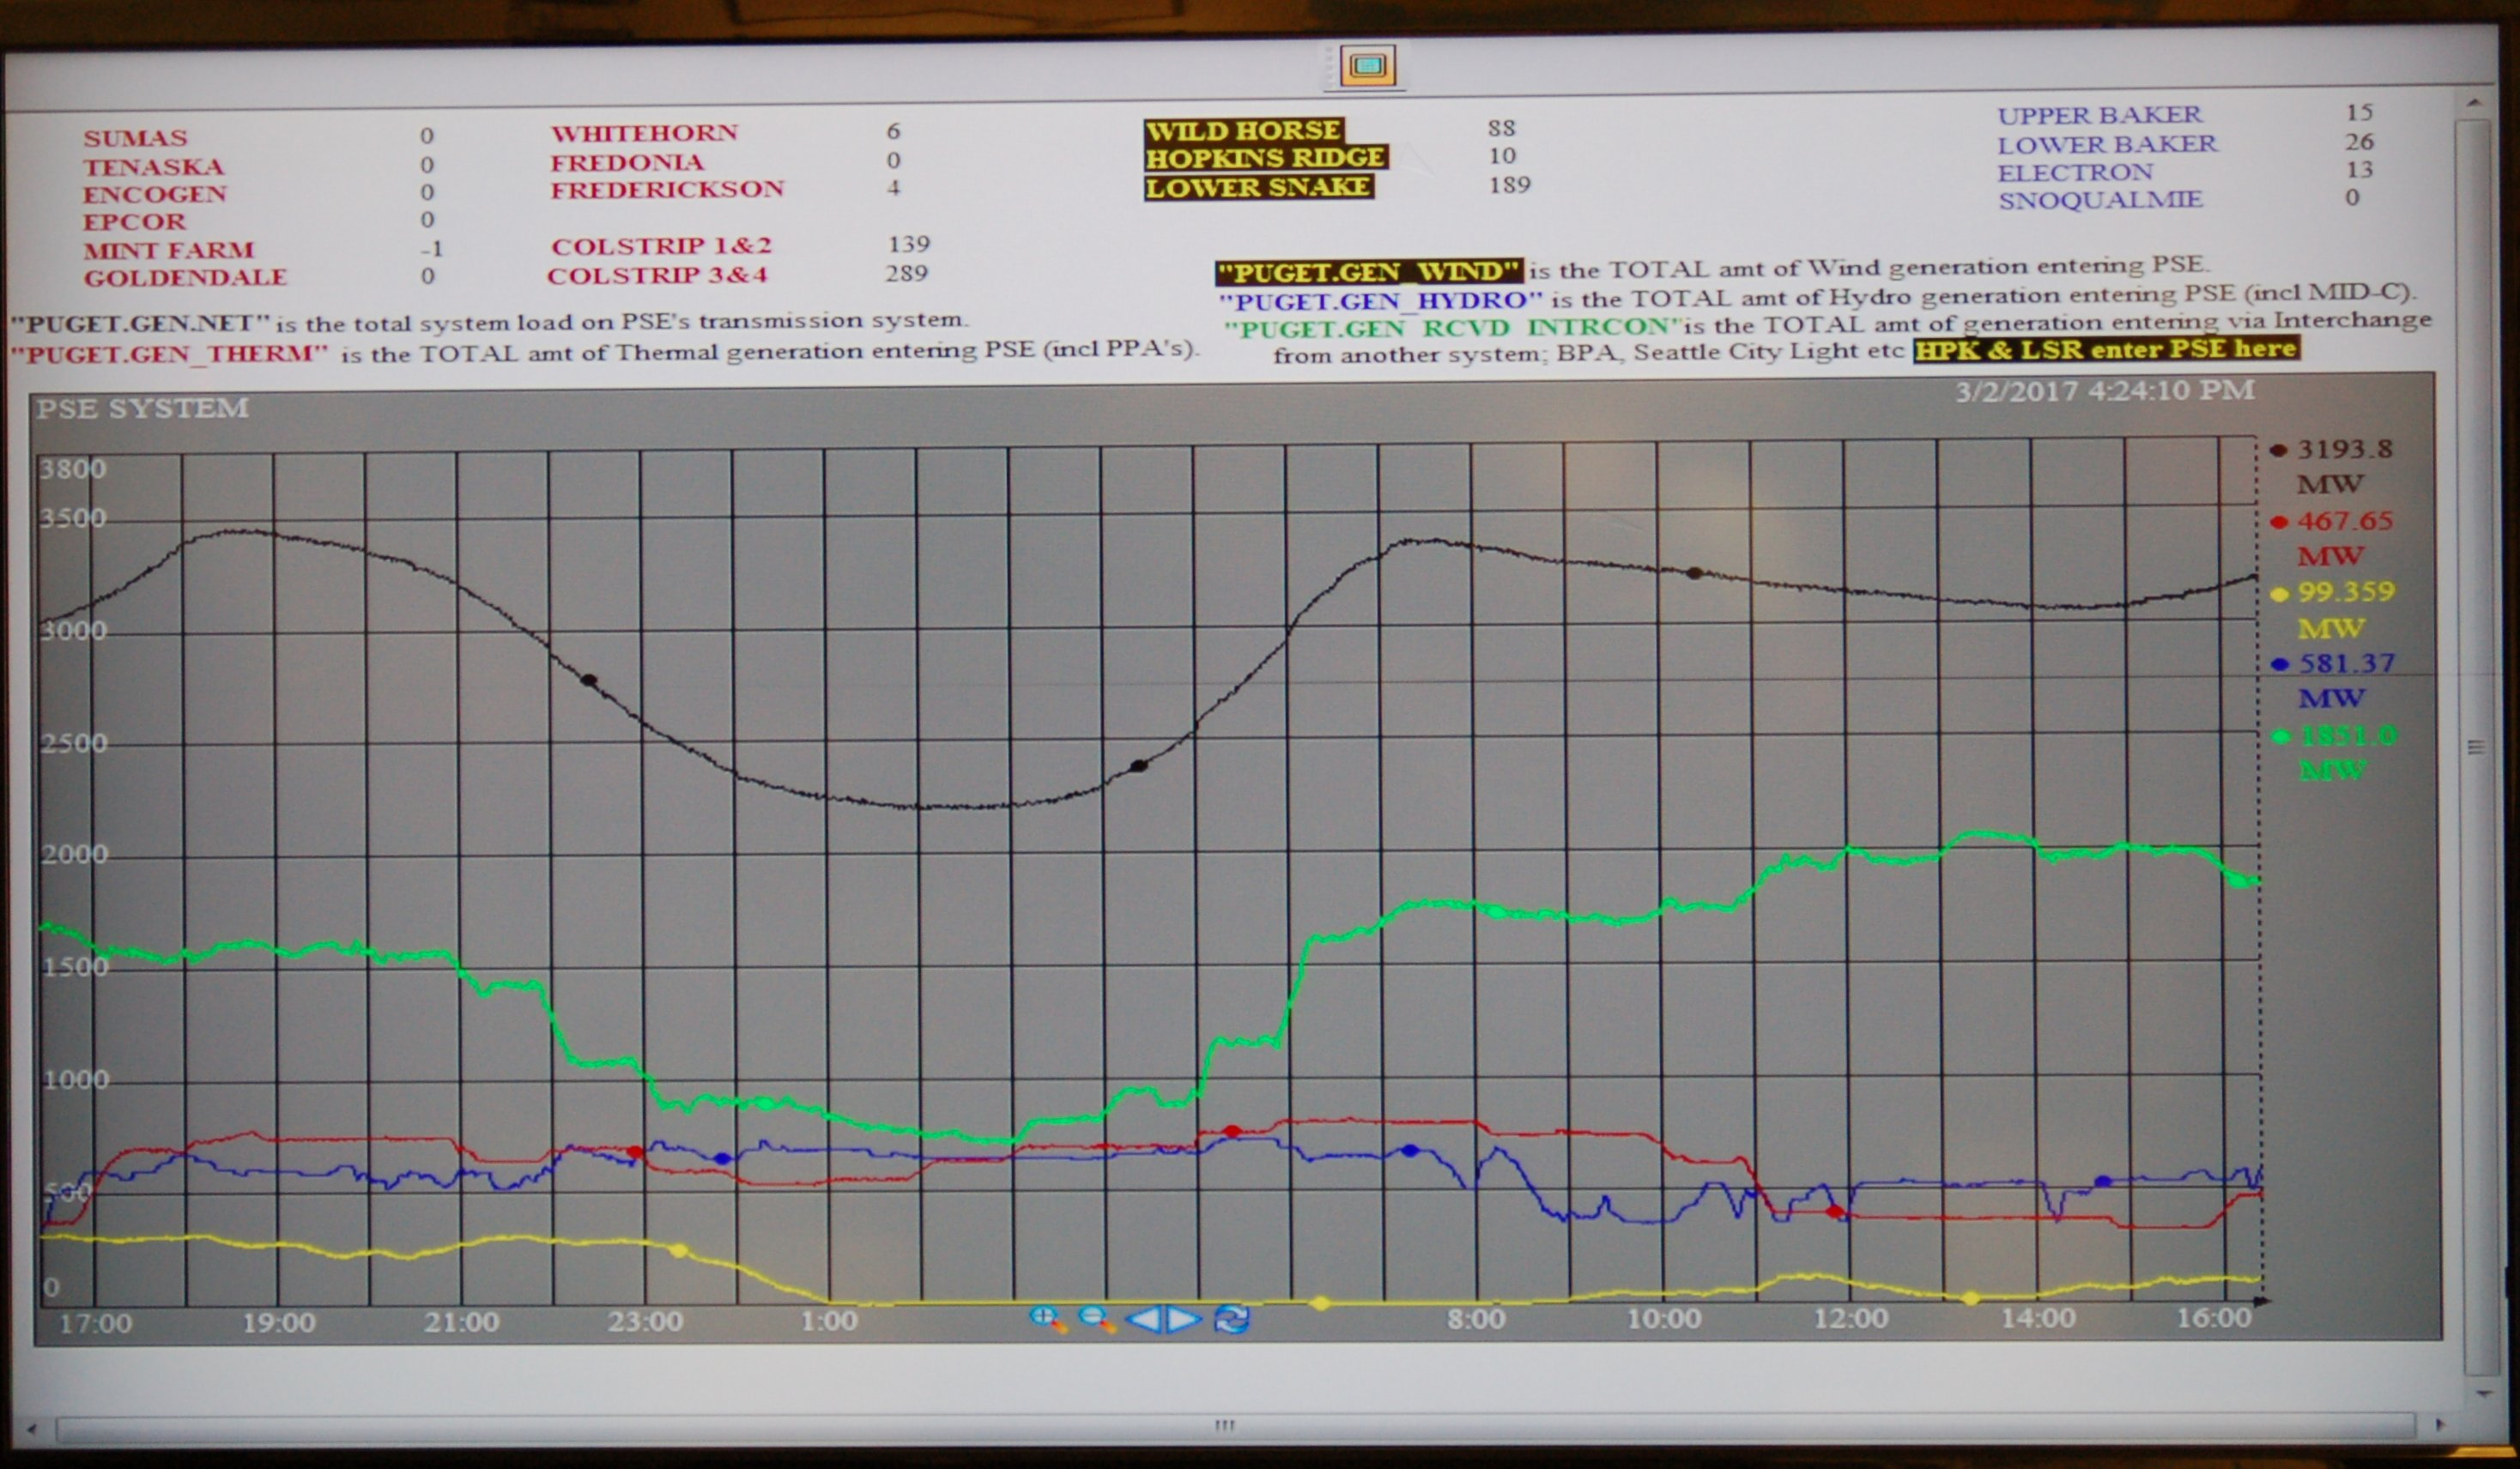
\includegraphics{power_173.eps}$$

Lines of differing color reveal power flow to and from this grid.  The black trend represents total \textit{load} on the system from all consumers: industrial, commercial, and residential.  Each of the other colored trends represent different sources of power to the grid.  Red represents thermal-based power plants, split between natural gas and coal energy sources.  Yellow represents wind turbine power generating stations, with zero output between the times of 1:00 AM and 8:00 AM on the graph (i.e. negligible wind blowing during that timespan).  Blue represents hydroelectric generators.  Finally, green represents power purchased from other electric utilities (e.g. Bonneville Power Administration and Seattle City Light).  \index{Bonneville Power Administration}  \index{Seattle City Light}

These trend graph reveals wind power to be a relatively small percentage of the total power generated during the timespan shown, with coal and hydroelectric sources remaining fairly constant over that time and the balance made up by power purchased from other utilities.

With no large-scale means to store excess electrical energy, the stability of an electrical grid depends on generating stations' ability to alter their power output to meet a continuously changing demand\footnote{Other options may exist for some grids.  For example, large-scale industrial customers may be requested to curtail their power consumption at certain times in order to offset a deficit in supply.  An example of this might be an aluminum smelter (which uses hundreds of megawatts of electricity to reduce alumina powder to molten aluminum metal) operating as a sheddable load while the same grid employs a nuclear fission power plant as one of its sources.  If the nuclear generator's reactor happens to ``scram'' (shut down for any reason), that reactor's power output will drop off the grid immediately, which may constitute hundreds of megawatts of lost generation.  In such an event, the grid dispatch system may issue a ``load shed'' command to the aluminum smelter to drop a substantial portion of its consumption, as it may not be practical to immediately bring that much extra power on-line from some other source.}.  Some types of generating stations lend themselves better to rapid changes in power output than others: single-cycle gas turbines, for example, excel at their ability to ramp power output up or down in relatively little time.  Steam-based thermal generators such as coal-fired power plants are not so tolerant.  Wind and solar generators operate at the whim of natural forces.

\vskip 10pt

Needless to say, modern electrical power grids are highly complex systems.  The critically important nature of a functioning power grid is difficult to overstate for any first-world nation, as so much depends on the uninterrupted flow of power from generating stations to customers.  The complexity of power grids and their control systems will only increase over time as more renewable generation capacity (e.g. wind and solar) is brought on-line to reduce overall dependency on non-renewable energy sources.  Large-scale energy storage systems will become a necessity for maintaining the stability of power grids dependent on power sources such as wind and solar that cannot be arbitrarily controlled.








\filbreak
\section{Interconnected generators}

Any power grid large enough to meet the demand of an entire nation must have multiple generators drawing from multiple energy sources supplying that power.  Connecting these generators together so as to equitably share loads in the grid is no trivial task.  The basic concepts involved with interconnecting generators, however, are independent of the distance separating those generators.  Thus, the examples given in this section are as relevant to generators located adjacent to each other as they are to generators located hundreds of miles apart.

\vskip 10pt

Let's begin with a simple electromechanical DC generator application, where one generator supplies power to one load.  Although not shown in this electrical schematic, there will be some form of ``prime mover'' such as an engine or a turbine turning the mechanical shaft of the generator:

$$\includegraphics{power_106.eps}$$

This system is almost too simple to warrant comment: the generator outputs a constant voltage, with load current being a function of load resistance in accordance with Ohm's Law ($I = {V \over R}$).  If load resistance happens to decrease and generator voltage remains constant, load current will increase as a result.  This additional load current has the effect of making the electromechanical generator harder to turn at the same shaft speed: demanding greater mechanical power input to the generator in order\footnote{This phenomenon is just one more application of the \textit{Law of Energy Conservation}, which states energy cannot be created or destroyed, but must be accounted for in all processes.  Every joule of energy delivered to the load in this example circuit must be supplied by the generator, which in turn draws (at least) one joule of energy from the prime mover (e.g. engine, turbine).  Since the power ``grid'' shown in this diagram has no means of storing energy for future use, the load's demand must be instantaneously met by the generator, and in turn by the prime mover.  Thus, sudden changes in load resistance result in instantaneous changes in power drawn from the prime mover, all in accordance with the Law of Energy Conservation.} to deliver greater electrical power to the load.  In this way the generator naturally ``senses'' the power demanded by the load.

\filbreak

Now, let us consider a second generator added in parallel to this simple power ``grid''.  In this configuration each of the two generators should contribute current to the grid, helping each other power the one load (resistor) shown on the right-hand side of the diagram:

$$\includegraphics{power_107.eps}$$

We know from basic circuit theory that parallel-connected components share the same voltage.  From this principle we may conclude that the two generators $V_1$ and $V_2$ will need to output the same amount of voltage in order to be compatible with each other in this circuit configuration.  To further explore this concept, we will consider what would happen if the two generator voltages were unequal to each other, including the resistance of the line connecting the two generators together:

$$\includegraphics{power_108.eps}$$

If the voltage of generator $V_1$ exceeds the voltage of generator $V_2$, the difference of those two generators' output voltages will be dropped along the length of the conductor $R_{line}$.  Ohm's Law allows us to predict the amount of current flowing through that line arising from the generators' differing output voltages ($I = {{V_1 - V_2} \over R_{line}}$).  If the voltage difference is substantial and the line resistance is minimal, this current will be quite large.  If this amount of current exceeds the amount drawn by the load, Kirchhoff's Current Law tells us the current through generator $V_2$ will be going the wrong direction: \textit{down} rather than \textit{up}.

This situation is undesirable because it means generator $V_2$ will actually be functioning as a \textit{load} rather than as the \textit{source} it should be.  Not only will generator $V_2$ not be contributing any power to the grid, but it will actually \textit{draw} power away from generator $V_1$ that could otherwise go to the load.  If generator $V_2$ is an electromechanical machine, it will operate as a motor as it draws power from generator $V_1$: ``motor'' $V_2$ increasing speed and generator $V_1$ slowing down from the additional loading.

To summarize: parallel-connected DC generators must output the same voltage in order to equitably share the burden of powering loads.  If one generator outputs less voltage than another, it will contribute less power.  if this disparity is great enough, the weaker generator will actually become a load and begin to function as an electric motor rather than the generator (source) it should be.

\vskip 10pt

\filbreak

Connecting AC generators in a power grid presents the same fundamental problem: all parallel-connected generators must output the same voltage to the ``grid'' in order to equitably share the load.  What makes AC generator interconnections more complex than DC generator interconnections is the fact that the voltage output by an AC generator is not a static quantity but rather is oscillating sinusoidally\footnote{The standard frequency for a power grid is typically 50 Hz or 60 Hz, depending on which part of the world you are in.  North American power grids typically operate at 60 Hz, while 50 Hz is more common in Europe.}.  This means paralleled AC generators must closely match one another's output voltage \textit{at every point along their sine-wave cycles} in order for them to productively work together on the grid.  The only way two or more AC generators may continuously match one another's output voltage is if their peak voltages are the same, their frequencies are the same, and they remain in-phase with each other.  

AC generator frequency is a direct function of shaft speed.  AC generator voltage is a direct function of shaft speed and rotor excitation current.  Thus, in order to connect two or more AC generators together, these two parameters must be precisely controlled.

The process of ensuring an AC generator is ready to be connected to a live grid is called \textit{synchronization}.  This may be done manually by human operators, or automatically by synchronization relays.  However it is done, the principle is the same: the voltage output by the un-synchronized generator is compared against the voltage of the grid, and the disconnecting switch or circuit breaker is not closed until the difference between those two voltages is nearly zero.  \index{Synchronization, generator}  \index{AC generator synchronization}  \index{Generator synchronization}

A simplified demonstration circuit serves to illustrate this process:  \index{Synchronization lamp}

$$\includegraphics{power_109.eps}$$

Imagine a condition where generator $V_1$ is operating and powering the load, but generator $V_2$ is stopped with its disconnecting switch in the open position.  In this condition the lamp will glow steadily, operating on the difference of potential between the power line (full AC voltage) and the idle generator $V_2$ (0 volts).

If we bring generator $V_2$ up to speed while keeping the disconnect switch in its open position, regulating the generator $V_2$'s output voltage and frequency to be equal to generator $V_1$, the lamp will experience a voltage strictly dependent on the degree of \textit{phase shift} between the two generators.  If, at this correct voltage and frequency, the phase of generator $V_2$ precisely matches the phase of generator $V_1$ (i.e. the sine-wave outputs of these two generators are in perfect lock-step with each other), the lamp will experience zero voltage and will remain dark.  If the two generators happen to be exactly 180 degrees out of phase with each other while maintaining equal voltage and frequency, the lamp will experience a sinusoidal voltage at that same frequency having a peak value \textit{twice} that of either generator, and will therefore glow at maximum brightness.  If the amount of phase shift between these two generators is any value between 0$^{o}$ and 180$^{o}$, the voltage experienced by the lamp will vary proportionately.  

\filbreak

If you imagine the two generators' voltages being phasors joined at the tails, the amount of voltage seen by the lamp will be equivalent to the distance between those two phasors' tips\footnote{A common analogy for this is two children swinging on adjacent swings in a playground.  Imagine the distance between the children being the amount of voltage difference between the two generators at any given point in time, with the amplitude of each child's swing representing the peak voltage of each generator and the pace of each child's oscillation being the frequency of each generator.  When two children are swinging in perfect synchronization, the distance between them remains minimal at all times.  When they swing 180$^{o}$ out of phase each other, the distance between them varies from minimal to maximal at a pace equal to the difference in their individual swinging rates.}:

$$\includegraphics{power_110.eps}$$ % Phasor diagram

If the two generators output different frequencies, the phase shift angle between them will not be constant.  Instead, the two generators will fall in and out of phase with each other at a frequency equal to the difference between the individual generator frequencies.  For example, if $V_1$ outputs 240 volts peak at 60 Hz and $V_2$ outputs 240 volts peak at 59 Hz, the two generators will roll in and out of phase with each other once per second (60 Hz $-$ 59 Hz = 1 Hz).  The lamp will thus experience an AC voltage that varies from 0 volts (when the two generators happen to be perfectly in phase) to 480 volts peak (when the two generators happen to be 180$^{o}$ out of phase).  In visual terms this means the lamp will alternate from complete darkness to full brightness and back again once per second.  Thus, the lamp's \textit{oscillation} serves to indicate the difference in frequencies between the two generators.

If the two generators output different amounts of voltage \textit{and} at different frequencies, the lamp will oscillate from bright to dim, never reaching full brightness or going completely dark.  Thus, the amount of \textit{variance in lamp intensity} serves to indicate the difference in voltage between the two generators.

The purpose of the lamp in this circuit, of course, is to indicate when it is safe to close the disconnect switch and tie generator $V_2$ to the power grid.  Since we know paralleled generators are electrically compatible only when their output voltages match at all times, we look for a condition of complete lamp darkness before closing the disconnect switch.

\vskip 10pt

Once the generators have been synchronized and the disconnect switch closed, an interesting phenomenon occurs: the two generators now behave as if their shafts were mechanically coupled\footnote{This ``coupling'' is not perfectly rigid, but does allow for some degree of phase difference between the generator and the grid.  A more accurate analogy would be to say the generators act as if their shafts were linked by a \textit{flexible} coupling.} together.  This is similar to the phenomenon experienced with the two parallel-connected DC generators shown earlier, where an under-performing generator would begin to ``motor'' and draw power from the stronger generator if their voltages were sufficiently different.  In the case of paralleled AC generators, a generator that begins to lag behind the other(s) in speed will act as a synchronous motor and draw power from the grid to match the speed of the other generator(s), staying in lock-step with the grid frequency so long as it is connected to the grid.  

If an AC generator is synchronized and connected to the grid, and then its prime mover's power is increased in an attempt to increase the shaft speed, that generator will in effect be trying to force all the other AC generators on that grid to a faster speed.  If the generator in question represents a small fraction of the grid's total power generating capacity as is typically the case, increasing or decreasing its speed becomes impossible\footnote{It should be noted that a grid-connected AC generator can in fact be over-sped with sufficient mechanical power input, but only if it ``slips a pole'' and falls out of synchronization as a result.  Such an event can be catastrophically to the offending generator unless it is immediately disconnected from the grid to avoid damage from overcurrent.} due to this coupling effect.  











\filbreak
\section{Single-line electrical diagrams}

Electrical power grids primarily consist of \textit{three-phase} AC circuits.  This means most power lines (transmission and distribution) have at least three conductors, and power transformers are either three-phase units or banks of single-phase transformers connected in Delta and/or Wye primary and secondary winding configurations.  Of course, diagrams must be drawn to document how all these conductors and power components interconnect, and standard electrical schematics serve that purpose well at the equipment level.  When analyzing power grids on the transmission or distribution scale, however, showing each and every conductor in electrical schematic form would make the system diagram needlessly complex.

For this reason electrical power grids are most commonly represented in a \textit{single-line diagram} format.  This means each transmission or distribution power line appears as a single line on the page, rather than as three (or four) lines showing individual conductors in a three-phase AC circuit.  Single-line diagrams work well to analyze the general flow of electrical power from sources to loads.

\vskip 10pt

\filbreak

The following schematic diagram represents a segment of an industrial power distribution system containing generators, power transformers, busses (sets of conductors used to connect multiple loads and/or sources in parallel with each other), instrument transformers\footnote{In this example, three \textit{current transformers}, or CTs, are shown stepping down the bus line current to levels safely measured by panel-mounted ammeters.  Current transformers typically step down line current to a nominal value of 5 amps to drive meters, relays, and other monitoring instruments.} and meters, circuit breakers, motors, and motor-starting switches:  \index{Current transformer (CT)}  \index{Bus, power system}

\vskip 10pt

\noindent
\textbf{Schematic diagram representation:}

$$\includegraphics[width=5in]{power_111.eps}$$

\vskip 10pt

\filbreak

A single-line diagram of the same industrial power distribution system shows all the same components:

\vskip 10pt

\noindent
\textbf{Single-line diagram representation:}

$$\includegraphics{power_112.eps}$$

Note how much simpler and ``cleaner'' the single-line diagram is compared to the schematic diagram of the same power system: each three-conductor set of power wires is shown as a single line, each transformer appears as a single primary winding and single secondary winding (rather than three of each), each motor and generator is a simple circle rather than a complete set of windings, motor starter contacts aren't triplicated, current transformers and ammeters appear as single units instead of triplets, and each three-pole circuit breaker appears as either a single square or a single breaker symbol.  For those familiar with industrial instrumentation and control system diagrams, the distinction between schematic diagrams and single-line diagrams is analogous to the distinction between loop diagrams and P\&IDs: the former shows a much greater degree of detail than the latter.  As with loop diagrams and P\&IDs for instrument technicians, schematic and single-line diagrams serve different purposes for professionals analyzing power systems.  There are circumstances when the intricate conductor-by-conductor detail of a schematic is necessary, but for quick analysis of operations and faults in large systems it is hard to compete with the elegance of a single-line diagram.

\vskip 10pt

A set of commonly-used single-line diagram symbols appears on the next two pages.

\filbreak

$$\includegraphics{diagrams09.eps}$$

\filbreak

$$\includegraphics{diagrams10.eps}$$

\filbreak

An example of a single-line diagram showing multiple generating stations, substations, transmission lines, and distribution lines appears here.  Note the coloring used to illustrate circuit breaker states (green = off and red = on) which is how single-line diagrams typically appear on computer-based SCADA system displays:  \index{SCADA}  \index{Supervisory Control And Data Acquisition}

$$\includegraphics{power_149.eps}$$

It should be abundantly clear from this example that the single-line diagram format greatly simplifies what would otherwise be a cluttered schematic diagram, in illustrating a system containing over a dozen generators and nearly as many loads.  As such, single-line diagrams are indispensable for electrical power system operators and other personnel who must make quick decisions in oversight of a power grid.









\filbreak
\section{Circuit breakers and disconnects}

\textit{Circuit breakers} are the ``final control elements'' of the electric power industry, akin to control valves in the process industries.  They are strictly on/off devices, used to make and break connections under load in power systems.  Circuit breakers automatically open when dangerous circuit conditions are detected.  Some low-voltage circuit breakers are strictly local-controlled devices, but larger circuit breakers (especially medium- and high-voltage units) may also be operated remotely by electrical signals.

\textit{Disconnects} are switches designed to isolate sections of a power system in case of damage or to allow for routine maintenance.  These may be manually-operated devices, or operated remotely by electric motor, and are typically not intended to make or break load current.  \textit{Circuit breakers}, by contrast, are designed to interrupt very high levels of electric current so they may safely cut off power in the event of a short-circuit fault.   \index{Disconnect, electrical power system}  \index{Circuit breaker}

This next photograph shows a set of three disconnect switches used on the line (input) side of a three-phase 500 kV power transformer bank in a large substation.  As you can see, each disconnect is a simple ``knife'' switch design, bearing a striking similarity to its electrical schematic symbol.  The long metal arm hinges on the left-hand side (at the top of the double insulator stands) and makes or breaks electrical contact on the right-hand side (where the arm is tipped with a sphere):

$$\includegraphics[width=5in]{power_20.eps}$$ % 500 kV disconnect switch

This particular high-voltage disconnect is motor-actuated, allowing all three disconnects to be operated in unison by remote control.  When in the ``open'' state each metal arm points vertically toward the sky, clearly revealing its status to visual inspection.  Lower-voltage disconnects are often built as manually-actuated devices, a crank handle or lever installed at ground level for a human lineman to actuate.

\filbreak

In series with these disconnect switches are a triad of 500 kV circuit breakers (with only two of them appearing in this next photograph).  The circuit-breaking elements reside in the horizontal tube portion of each unit (called the ``tank''), the tall ribbed structures being insulated conductors bringing the power down to the low-mounted breaker tank.  Since disconnect switches are generally not rated for load current interruption, circuit breakers are necessary to ``break'' the current and safely extinguish the inevitable arc that forms when a live circuit is broken.  In the background you can see a hinged disconnect switch in series with the furthest circuit breaker, a set of which serve to isolate power from the three circuit breakers (and every other component ``downstream'' of the disconnects) to permit maintenance on those components:

$$\includegraphics[width=5in]{power_19.eps}$$ % 500 kV live-tank circuit breaker

All three circuit breakers are remotely controlled by 125 VDC signals energizing solenoid coils within the breaker units.  One solenoid coil called the ``close'' coil causes the breaker mechanism to move to the closed (conducting) position when momentarily energized.  Another solenoid coil called the ``trip'' coil causes the breaker mechanism to move to the open (non-conducting) position when momentarily energized.  The breakers also contain status contacts signaling the breaker's change of state.  It is these solenoid coils and status contacts which permit the circuit breaker to be a part of an automatic control system rather than function merely as a manual switching device.







\filbreak
\subsection{Low-voltage circuit breakers}

This photograph shows a typical low-voltage\footnote{In the United States, the term ``low voltage'' with reference to power circuits usually refers to circuits of 600 volt or less potential.} (480 volt) circuit breakers in a ``Motor Control Center'' (MCC) panel, for 480 volt 3-phase industrial power circuits:  \index{Motor control center (MCC)}  \index{MCC room}

$$\includegraphics[height=6in]{power_21.eps}$$

Note how each circuit breaker has its own on/off handle, for manual operation.  These circuit breakers, like most low-voltage breakers, are capable of turning off (``tripping'') on their own when high current is detected, but must be turned on (``closed'') manually.  That is to say, they lack ``close'' and ``trip'' solenoid coils present in larger circuit breaker units which would permit remote operation.

Some low-voltage circuit breakers utilize thermal elements to detect overcurrent conditions, much like the circuit breakers traditionally found in residential applications.  When this thermal element inside the circuit breaker becomes too warm with current, it mechanically forces the mechanism to trip and open the contacts.  Other low-voltage circuit breakers are magnetically operated, tripping when the magnetic field caused by conductor current becomes excessive.  In either case, the trip mechanism for a low-voltage circuit breaker is typically contained within the circuit breaker itself.

%ADD: Low-voltage circuit breakers use air as the insulating medium between open contacts.  The arc produced by a contact opening under a condition of high current can reach extremely high temperatures, and poses an operating hazard to personnel working near the breaker unit.

\vskip 10pt

\filbreak

A close-up photograph shows one of these breaker panels, containing two separate three-phase circuit breakers inside:

$$\includegraphics[width=5in]{power_22.eps}$$

Note how the ``Sump Pump'' circuit breaker has been placed in the ``off'' position, its handle locked there by a padlock, a danger tag attached to notify any personnel of the reason for the breaker's lock-out.  \index{Lock-out, tag-out}  \index{LOTO}

\filbreak

This next photograph shows a different brand of MCC (manufactured by Gould) where each unit contains not only a circuit breaker, but also an entire motor starter assembly (contactor, overload heaters, and associated switch contacts) for controlling a three-phase electric motor.  One of these motor control ``buckets'' has been removed, revealing the line and load bus connections in the rear:  \index{Contactor}

$$\includegraphics[height=4in]{power_100.eps}$$

Industrial circuit breakers such as this are typically designed to be unplugged for ease of maintenance and replacement.  If the ``bucket'' units are heavy, a lifting hoist is provided on the MCC to facilitate their removal and replacement.




\filbreak
\subsection{Medium-voltage circuit breakers}

Circuit breaker design and construction becomes more complicated at higher voltages, such as the voltage range extending from 2.4 kV to 35 kV commonly classified as ``medium-voltage'' in the electrical power distribution industry.  Aside from being physically larger than low-voltage circuit breakers, medium-voltage circuit breakers are generally not self-tripping as low-voltage circuit breakers are.  Rather, medium-voltage circuit breakers are electrically commanded to trip (and to close) by external devices called \textit{protective relays} monitoring dangerous electrical conditions.  Internally, these circuit breakers are equipped with ``trip'' and ``close'' electromagnet solenoids allowing the mechanism to be triggered by remote electrical signals.  \index{Protective relay}  \index{Medium-voltage circuit breaker}

Medium-voltage circuit breakers are designed to be unplugged from the breaker panel for maintenance and replacement.  This is referred to in the electrical power industry as \textit{racking out} a circuit breaker.  Some circuit breakers ``rack'' by moving horizontally, sliding in and out of the panel on guide rails.  Other circuit breakers ``rack'' by moving vertically, sliding up into and down out of the stationary panel terminals, as shown in the following illustration: \index{Racking out, circuit breaker}

$$\includegraphics{power_67.eps}$$

The primary purpose of being able to ``rack'' a medium voltage breaker into and out of its place in a breaker panel is to facilitate regular maintenance on the circuit breaker mechanism.  Unlike the circuit breakers you find in your home, these units may be frequently cycled and will suffer definite wear with each actuation.  After a certain number of closing/tripping cycles, the breaker must be removed from service for inspection and testing.  

Racking out a circuit breaker also provides another advantage, and that is an extra measure of safety when securing a power circuit in a zero-energy state.  When a circuit breaker has been locked into its ``racked out'' position, the load conductors serviced by this breaker absolutely cannot become energized even if the circuit breaker contacts were made to close.  This is analogous to unplugging an electrical appliance from a wall receptacle: it cannot be powered up even if the switch is turned on!

\filbreak

An example of a vertically-racking circuit breaker is the General Electric ``Magneblast'' unit shown below, designed for use in power systems operating up to 15 kV.  The particular unit shown rests on a wooden pallet in a storage area.  Normally, it would be installed in a metal-clad breaker panel, its components hidden from direct view:  \index{General Electric ``Magneblast'' circuit breaker}

$$\includegraphics[height=4in]{power_23.eps}$$

The six ``stabs'' seen on the top of this breaker unit engage with six sockets connected to the six bus-bar conductors inside the breaker panel (three for the three phases of the line supply, plus three more for the three phases of the load conductors).  When this circuit breaker is ``racked out,'' it is dropped down so that these six stabs disengage from the bus-bar connections, making it impossible to energize the load conductors even if the breaker contacts close.

A detail not seen in this photograph is the hoisting mechanism necessary to lift this breaker into its ``racked-in'' position.  Medium-voltage circuit breakers such as the General Electric Magneblast are quite heavy, requiring special ``lift truck'' frames to hoist into and out of their engaged positions in the circuit breaker panel. 

\filbreak

Not only does ``racking out'' a circuit breaker add an extra measure of safety for personnel working on the load circuit, but it also allows the breaker to be tested in-place without energizing the load.  The electrical connections commanding the breaker to open (trip) and close may still be connected to the control circuitry even in the racked-out state, permitting such tests.  The following illustration shows how such a test may be performed in the ``racked-out'' condition:

$$\includegraphics{power_68.eps}$$

\vskip 10pt

At medium-voltage and greater levels of potential, a significant design problem is how to rapidly extinguish the arc formed when contacts separate under load.  Low-voltage circuit breakers simply rely on a wide and rapid enough separation of contact points to ensure the electric arc formed when the breaker trips cannot continue more than a fraction of a second.  In medium-voltage circuits, both the heat output and the potential length of the electric arc formed by separating contacts is huge and therefore the arc must be extinguished as quickly as possible, both for personnel safety and for extending the operating life of the circuit breaker.

The original General Electric Magneblast circuit breaker design used a series of \textit{arc chutes}, electromagnet coils, and pneumatic jets to direct the arc away from the separating contacts and thereby extinguish it rapidly.  Other medium-voltage circuit breaker designs submerge the electrical contacts in an \textit{oil bath} to keep them completely isolated from air so that an arc could never form.  This oil has a high dielectric value (i.e. it is an excellent electrical insulator with a high breakdown rating), but needs to be tested on a regular basis to ensure good integrity.  \index{Arc chute, circuit breaker}

\filbreak

A modern approach to the problem of extinguishing the arc drawn by opening circuit breaker contacts is to encapsulate the contacts inside of an air-tight \textit{vacuum chamber}.  This rear view of this GE Magneblast circuit breaker shows it retrofitted with vacuum contacts (the three white-colored components seen inside the breaker frame), replacing the old open-air contacts and arc chutes:  \index{Vacuum circuit breaker}

$$\includegraphics[height=4in]{power_24.eps}$$

By removing all air from the vicinity of the contacts, there are no gas molecules to ionize when the contacts separate.  Not only does this completely eliminate the problem of contact arcing, but it also permits the circuit breaker mechanism to perform its job with a shorter ``throw'' (less contact motion), since less gap distance is necessary to prevent current in a vacuum than in air.  The only real challenge now is ensuring the integrity of the vacuum inside these chambers.  This requires periodic testing of the contacts' dielectric rating by maintenance personnel using high-voltage testing equipment.

\vskip 10pt

\filbreak

An interesting feature of the GE Magneblast and other medium-voltage circuit breakers is the mechanism for actuation.  These circuit breaker contacts must be moved swiftly and with significant force in order to ensure quick and repeatable make/break times.  In order to achieve this rapidity of motion, the breaker is designed to actuate by the stored energy of large mechanical springs.  A side-view of a Magneblast circuit breaker shows a pair of large coil springs used to trip and close the circuit breaker contacts:

$$\includegraphics[width=4in]{power_25.eps}$$

Much like the spring on the hammer of a firearm, the springs inside this Magneblast circuit breaker provide the mechanical driving force for opening and closing the breaker's three electrical power contacts.  The act of opening or closing this circuit breaker is analogous to pulling the trigger of a firearm: a small mechanical movement unleashes the stored energy of these springs to do the actual work of rapidly opening and closing the contacts.

\filbreak

These springs are tensed (``charged'') by an electric motor in the times following an actuation cycle, so they will be ready for the next actuation.  Typically these charging motors are powered by 125 VDC supplied by the substation's ``station power'' battery bank, so they may operate even in the event of a total black-out condition where the substation loses AC line power from its incoming transmission lines.  Indicator flags on the front of the circuit breaker reveal the breaker's contact status as well as its spring charge status:

$$\includegraphics[height=5in]{power_26.eps}$$

Green-colored flags seen on the front panel of this breaker show the contact status as ``open'' and the spring status as ``discharged''.  This circuit breaker is incapable of any action until its spring is charged.  Once the spring has been charged, pushing the button labeled ``Manual trip'' will cause the breaker contacts to open, and pushing the button labeled ``Manual close'' will cause the breaker contacts to close.

\filbreak

A photograph of the front panel of a Westinghouse vacuum circuit breaker reveals the same basic indicators and manual controls seen on the (older) General Electric circuit breaker:

$$\includegraphics[width=5in]{power_35.eps}$$

In this particular example, the actuating spring is charged, which means the breaker is in a state of readiness to switch from its present status (open, or tripped) to its opposite status (closed).

Both of these medium-voltage circuit breakers share another feature of interest: a mechanical counter tracking the number of close/trip cycles the breaker has experienced.  The act of making and breaking high-power electric circuits takes a toll on the components of a circuit breaker -- especially the contacts -- and therefore this count value is a useful parameter for maintenance purposes.  The breaker should be serviced at manufacturer-specified intervals of close/trip cycles, just like an automobile should be serviced at manufacturer-specified intervals of distance traveled.












\filbreak
\subsection{High-voltage circuit breakers}

At voltages 46 kV and above (classified as ``high voltage'' in the electrical power industry), the challenge of extinguishing the electric arc formed by separating breaker contacts becomes severe.  Two popular strategies for mitigating contact arc in modern high voltage circuit breakers are \textit{oil immersion} and \textit{gas quenching}.  \index{High-voltage circuit breaker}

A set of three oil-bath circuit breakers (OCB's) rated for 230 kV service is shown here, retired from service:

$$\includegraphics[height=5in]{power_28.eps}$$

Each of the three circuit breakers (one for each line of the three-phase circuit) is mechanically linked by a common shaft at the top of the breaker tanks, so they all trip and close as one unit.

The fast and reliable actuation of such a bulky mechanism requires a large amount of stored energy, and in the case of the oil circuit breaker shown above the energy storage medium is compressed air.  An on-board electric air compressor powered by ``station power'' maintains air pressure inside a pressure vessel, and this compressed air is directed to a piston actuator through solenoid valves to provide the actuation force necessary to move the breaker contact assemblies open and closed.

\filbreak

A view inside the enclosure on the far side of this oil circuit breaker reveals the air compressor (upper-right), compressed air storage tank (right) and actuation cylinder (middle):

$$\includegraphics[width=5in]{power_29.eps}$$

The man shown in this photograph is pointing to a solenoid valve designed to pass compressed air to and from the piston actuator.  A large-diameter black hose runs from this solenoid through the bottom of the enclosure, allowing compressed air from the cylinder to vent to atmosphere.

\filbreak

A more modern breaker design for 230 kV service is this gas-quenched circuit breaker unit, a mere fraction\footnote{For an equitable size comparison between the two different types of circuit breaker, consider the fact that the insulators on this gas-quenched circuit breaker are approximately the same physical height as the insulators on the previously-shown oil-tank circuit breaker.} of the physical size of the oil circuit breaker shown previously:

$$\includegraphics[width=5in]{power_30.eps}$$

The ribbed porcelain structures are the high-voltage terminals for this circuit breaker: three for the three-phase lines coming in, and three for the three-phase load terminals exiting.  The actual contact assemblies reside in the gas-filled horizontal metal tubes (``tanks'').  It is striking to note that the same current interruption and isolation functions performed by the gigantic oil-filled tanks of the retired circuit breaker previously shown are performed by this relatively tiny gas-quenched breaker.

The gas inside the breaker's tanks is \textit{sulfur hexafluoride}, a very dense gas (about 5 times denser than air) with excellent electrical insulating and arc-extinguishing properties.  SF$_{6}$ gas is contained in these breaker contact chambers under pressure to maximize its dielectric breakdown strength (its ability to withstand high voltage without ionizing and passing current across the gap between the circuit breaker's open contacts).  SF$_{6}$ gas is non-toxic\footnote{While pure SF$_{6}$ gas is benign, it should be noted that one of the potential chemical byproducts of arcing in an SF$_{6}$-quenched circuit breaker is hydrofluoric acid (HF) which is extremely toxic.  HF is formed when SF$_{6}$ gas arcs in the presence of water vapor (H$_{2}$O), the latter being nearly impossible to completely eliminate from the interior chambers of the circuit breaker.  This means any maintenance work on an SF$_{6}$-quenched circuit breaker must take this chemical hazard into consideration.} and safe to handle.

\filbreak

Like the large oil-filled circuit breakers seen previously, this SF$_{6}$ circuit breaker has an enclosure on one side where the actuation and control components are located.  Inside this enclosure we see a large stack of Belleville spring washers (the dark-colored discs located in the center of the enclosure), which are used as the mechanical energy-storage medium instead of compressed air.  This stack of spring-steel washers is compressed by an electric motor and gear mechanism, then the spring tension is released through another mechanism to close and trip the breaker's contacts on demand.  As usual this charging motor receives its power from the uninterruptible ``station power'' supply of the substation, allowing the breaker to actuate even in the event of a total ``blackout'' condition:  \index{Belleville washer spring}

$$\includegraphics[width=5in]{power_31.eps}$$

Inside this enclosure we also see a small pair of pushbuttons (one red, one green) just below and to the right of the Belleville washer stack for manually closing and tripping the breaker, respectively.  The common color coding used in the United States for electric power switchgear is \textit{red for energized}, \textit{green for de-energized}.  This may seem backward to most people familiar with red and green traffic lights, where red means ``stop'' and green means ``go,'' but the concept here is one of safety: red means ``dangerous'' (power on) while green means ``safe'' (power off).

It should be noted that most of the time these high-voltage circuit breakers are triggered remotely, rather than manually by someone standing near them.  These command signals may come from a manual switch located in the control room, or from some automatic circuit such as a \textit{protective relay} instructing the breaker to open due to an abnormal system condition.

\filbreak

The nameplate photographed on a similar SF$_{6}$ circuit breaker reveals some interesting features:

$$\includegraphics[width=6in]{power_36.eps}$$

According to this nameplate, the normal operating pressure for the SF$_{6}$ gas is 98.6 PSI.  A low-pressure alarm triggers if the SF$_{6}$ gas pressure happens to fall below 85 PSI.  When opening (tripping), the circuit breaker only takes \textit{3 cycles'} worth of time at 60 Hz to completely interrupt the current.  One solenoid coil closes the breaker, and that coil requires a signal of 125 volts DC at just over 3 amps of current.  The breaker's contacts may be tripped by energizing one or more redundant solenoid coils at 125 VDC and 1.8 amps (each).  In either direction, the breaker's actuation is powered by a pre-charged spring, much like the 230 kV breaker seen previously.  This particular breaker is rated for 123 kV at 2000 amps full-load.

\vskip 10pt

\filbreak

Sulfur hexafluoride gas circuit breaker technology is popular for higher voltage applications as well, such as these 500 kV circuit breakers seen here:

$$\includegraphics[width=5in]{power_32.eps}$$

In this application, where three separate circuit breaker units independently interrupt current for the three-phase power lines, there is no mechanical link to synchronize the motion of the three contact sets.  Instead, each single-phase circuit breaker actuates independently.

\filbreak

%An electronic synchronizing control system is used to coordinate the closing and tripping of these three circuit breakers, seen here in this photograph where the enclosure's door has been opened for inspection:

%$$\includegraphics[width=5in]{power_33.eps}$$

%\filbreak

%This synchronous control unit monitors both voltage and current for the three circuit breakers, via PT (``potential transformer'') and CT (``current transformer'') instrument transformers.  The PT and CT signal wire connections may be seen at the top of the panel on the synchronizing unit:

%$$\includegraphics[width=5in]{power_34.eps}$$

%In order to minimize contact arcing, each breaker contact should be closed when the voltage across its contact is such that the current will be minimized\footnote{For resistive and capacitive loads, this means closing the contact at the point of voltage zero-crossing (when the voltage waveform passes through 0 volts).  For inductive loads such as shunt reactors and unloaded transformers, this means closing the contact at the point where voltage is at its peak value (i.e. where the reactive, lagging current waveform would be at zero-crossing).}, and each breaker contact should be opened (tripped) when the current through the contact is near zero.  The synchronizing unit not only monitors the AC voltage and current status for each breaker's contact, but it also ``learns'' the average actuation time for each circuit breaker mechanism by measuring the time delay between the trigger signal and the change in current signifying contact opening or closing.  In this way, the synchronizer is able to anticipate when the AC voltage or current value will cross zero, and send a triggering signal to each breaker mechanism at precisely the right time so all three breaker contacts experience minimum arcing.

So far all of the high-voltage circuit breakers shown in previous photographs are of the \textit{dead tank} type, where the structure housing the interrupting contact(s) is maintained at ground potential (i.e. the outside surface of the circuit breaker mechanism is electrically ``dead'').  Some high-voltage circuit breakers are built such that their interrupting assemblies are at line potential, the entire breaker suspended above ground from insulators.  This type of circuit breaker is called a \textit{live tank}, because the ``tank'' containing the contact(s) operates at a high voltage with respect to earth ground.  A photograph of a 500 kV, single-pole\footnote{This particular circuit breaker, like most live-tank circuit breakers, interrupts just one phase (i.e. one ``pole'') of a three-phase bus.  Portions of the second and third live-tank SF$_{6}$ breakers comprising the full three-phase breaker array for this bus may be seen near the left-hand edge of the photograph.}, SF$_{6}$-quenched, live tank breaker appears next:

$$\includegraphics[height=5in]{power_118.eps}$$

The actuating mechanism for this live-tank breaker is housed in the ``can'' assembly seen at the base, where the vertical insulator meets the steel supporting tower.

\vskip 10pt

\filbreak

Another 500 kV, single-pole, live-tank circuit breaker assembly appears in the next photograph, this particular breaker being an older unit using \textit{compressed air} as the interrupting medium rather than sulfur hexafluoride gas:

$$\includegraphics[width=5in]{power_119.eps}$$

Air nozzles powered by hundreds of PSI of compressed air are used to ``blow out'' the arc formed when the circuit breaker's contacts separate.  These air nozzles are not visible in the photograph, being internal to the circuit breaker's construction.  An interesting feature of this style of circuit breaker is the loud report generated when it trips: the sound of the compressed air jets extinguishing the arc across the separating contact poles within the breaker is not unlike that of a firearm discharging.  

Multiple series-connected contact assemblies comprise this circuit breaker, distributing the energy of the arc across multiple points in the breaker assembly rather than across a single contact.  This is evident in the photograph as multiple clusters of ``tanks'' on the top of the left-hand assembly, as well as the second live-tank assembly connected in series to the right.  Such arrangements are necessary because air is a less effective medium for extinguishing an electric arc than either oil or SF$_{6}$ gas.









\filbreak
\subsection{Reclosers}

A special type of medium-voltage circuit breaker used to quickly interrupt and re-establish power in distribution lines is called a \textit{recloser}.  Reclosers are designed to trip if ever a distribution line suffers a ``transient'' (momentary) fault due to some natural event such as a lightning strike causing an insulator to ``flash over'' to ground or a tree branch touching one or more line conductors, then automatically re-close moments later to test whether or not the fault still persists.  If the fault clears on its own -- a common occurrence with tree branches, as the branch may break off or burn away following the initial arc -- then the recloser remains closed and continues providing power to customers.  By some estimations transient faults account for 70\% to 90\% of all faults occurring on overhead power lines.  If non-reclosing fault protection were applied to all distribution and transmission lines, extended interruptions of electric power service would be far more common than they are now.  \index{Flashover, power line insulator}  \index{Transient fault, power line}

If you have ever experienced momentary cessations of electrical power service to your home or business where the power ``blinks'' off and on in rapid succession, you have experienced a recloser at work.  The recloser opens as soon as an overcurrent condition is detected, then recloses briefly to ``test'' for continued presence of the fault.  If the fault persists, the recloser trips again and then recloses once more to ``re-test'' for the fault.  If the fault has cleared by then, the recloser remains closed and restores normal power service to customers.  Only if the fault persists after multiple ``shots'' does the recloser remain in the tripped (open) state and waits for line crews to repair the fault.

Reclosers are typically located some distance ``downstream'' of the substation, to isolate certain remote portions of the distribution network.  Circuit breakers at the substation provide protection for each distribution line as a whole:

$$\includegraphics{power_114.eps}$$

\vskip 10pt

\filbreak

A typical recloser resembles a ``circuit breaker on a stick,'' located near the top of a distribution power pole near the line conductors.  Modern reclosers use SF$_{6}$ gas quenching to extinguish arcing resulting from the interruption of high-magnitude fault currents.  Legacy reclosers typically employed oil quenching.  This photograph shows a modern (SF$_{6}$-quenched) recloser, with its three phase current-interrupting contact units clearly visible:

$$\includegraphics[height=4in]{power_113.eps}$$

The grey enclosure located near ground level on this pole contains the \textit{protective relay} responsible for issuing the ``trip'' and ``close'' signals to the recloser's coils.  Current transformers located within the recloser provide isolated sensing of line current to the reclosing relay, necessary for detecting any overcurrent conditions that might result from a transient fault.  Each attempt by the reclosing relay to re-close the breaker is called a \textit{shot}.  If the reclosing relay fails to clear the fault by a certain number of shots, it enters the \textit{lockout} state whereby the recloser remains open and must be re-closed by human intervention.

\vskip 10pt

Distribution line reclosers, unlike circuit breakers located in substations, cannot rely on an auxiliary ``station power'' energy source for opening and closing its line-interrupting contacts.  Therefore these small units utilize AC line voltage as the actuating power for the contacts.  Low-voltage ``trip'' and ``close'' circuits still exist for control purposes, but the actual energy source for rapid tripping/reclosing cycles comes from the AC line itself.

\vskip 10pt

The principle of automatic reclosing may be applied to transmission lines as well as distribution lines, but new challenges exist at this level of a power grid.  When transmission lines serve to interconnect distributed generating stations, interruption of that line for any significant time invites generator de-synchronization.  Recall that AC generators, once synchronized with each other and connected in parallel on a common grid circuit, tend to remain synchronized with each other as though their mechanical shafts had become coupled.  If a circuit breaker opens along a transmission line system and de-couples generators from each other, those generators will be free to fall out of synchronization.  Reclosing that circuit breaker when those generators are out of sync with each other can be disastrous.  Automatic reclosing at the distribution line level of a power grid, therefore, must either be fast enough that generators will not have enough time to fall out of sync with each other, or blocked by other protective relay logic to prevent reclosure in an out-of-sync situation.










\filbreak
\section{Electrical sensors}

The two ``process variables'' we rely on most heavily in the field of electrical measurement and control are \textit{voltage} and \textit{current}.  From these primary variables we may determine impedance, reactance, resistance, as well as the reciprocals of those quantities (admittance, susceptance, and conductance).  

Other sensors more common to general process measurement such as temperature, pressure, level, and flow are also used in electric power systems, but their coverage in other chapters of this book is sufficient to avoid repetition in this chapter.

Two common types of electrical sensors used in the power industry are \textit{potential transformers} (PTs) and \textit{current transformers} (CTs).  These are precision-ratio electromagnetic transformers used to step high voltages and high currents down to more reasonable levels for the benefit of panel-mounted instruments to receive, display, and/or process.




\filbreak
\subsection{Potential transformers}

Electrical power systems typically operate at dangerously high voltage.  It would be both impractical and unsafe to connect panel-mounted instruments directly to the conductors of a power system if the voltage of that power system exceeds several hundred volts.  For this reason, we must use a special type of step-down transformer referred to as a \textit{potential transformer} to reduce and isolate the high line voltage of a power system to levels safe for panel-mounted instruments to input.

Shown here is a simple diagram illustrating how the high phase and line voltages of a three-phase AC power system may be sensed by low-voltage voltmeters through the use of step-down potential transformers:

$$\includegraphics{power_04.eps}$$

Potential transformers are commonly referred to as ``PT'' units in the electrical power industry.  It should be noted that the term ``voltage transformer'' and its associated abbreviation VT is becoming popular as a replacement for ``potential transformer'' and PT.  \index{Potential transformer (PT)}  \index{PT, potential transformer}  \index{Voltage transformer (VT)}  \index{VT, voltage transformer}

\vskip 10pt

When driving a voltmeter -- which is essentially an open-circuit (very high resistance) -- the PT behaves as a voltage source to the receiving instrument, sending a voltage signal to that instrument proportionately representing the power system's voltage.

\filbreak

The following photograph shows a potential transformer sensing the phase-to-ground voltage on a three-phase power distribution system.  The normal phase voltage in this system is 7.2 kV (12.5 kV three-phase line voltage), and the PT's normal secondary voltage is 120 volts, necessitating a ratio of 60:1 (as shown on the transformer's side):

$$\includegraphics[width=4in]{power_01.eps}$$

Any voltage output by this PT will be $1 \over 60$ of the actual phase voltage, allowing panel-mounted instruments to read a precisely scaled proportion of the 7.2 kV (typical) phase voltage safely and effectively.  A panel-mounted voltmeter, for example, would have a scale registering 7200 volts when its actual input terminal voltage was only 120 volts.  This is analogous to a 4-20 mA indicating meter bearing a scale labeled in units of ``PSI'' or ``Degrees Celsius'' because the 4-20 mA analog signal merely represents some other physical variable sensed by a process transmitter.  Here, the physical variable being sensed by the potential transformer is still voltage, just at a 60:1 ratio greater than what the panel-mounted instrument receives.  Like the 4-20 mA DC analog signal standard so common in the process industries, 115 or 120 volts is the standard potential transformer output voltage used in the electrical industry to represent normal power system voltage.

This next photograph shows a set of three PTs used to measure voltage on a 13.8 kV substation bus.  Note how each of these PTs is equipped with \textit{two} high-voltage insulated terminals to facilitate phase-to-phase (line voltage) measurements as well as phase-to-ground:

$$\includegraphics[width=4in]{power_146.eps}$$

\filbreak

Another photograph of potential transformers appears here, showing three large PTs used to precisely step the phase-to-ground voltages for each phase of a 230 kV system (230 kV line voltage, 133 kV phase voltage) all the way down to 120 volts for the panel-mounted instruments to monitor:

$$\includegraphics[height=5in]{power_02.eps}$$

A loose-hanging wire joins one side of each PT's primary winding to the respective phase conductor of the 230 kV bus.  The other terminal of each PT's primary winding connects to a common neutral point, forming a Wye-connected PT transformer array.  The secondary terminals of these PTs connect to two-wire shielded cables conveying the 120 volt signals back to the control room where they terminate at various instruments.  These shielded cables run through underground conduit for protection from weather.

Just as with the previous PT, the standard output voltage of these large PTs is 120 volts, equating to a transformer turns ratio of about 1100:1.  This standardized output voltage of 120 volts allows PTs of any manufacture to be used with receiving instruments of any manufacture, just as the 4-20 mA standard for analog industrial instruments allows ``interoperability'' between different manufacturers' brands and models.

\filbreak

A special form of instrument transformer used on very high-voltage systems is the \textit{capacitively-coupled voltage transformer}, or CCVT.  These sensing devices employ a series-connected set of capacitors dividing the power line voltage down to a lesser quantity before it gets stepped down further by an electromagnetic transformer.  A simplified diagram of a CCVT appears here, along with a photograph of three CCVTs located in a substation:  \index{Capacitively-coupled voltage transformer (CCVT)}  \index{CCVT, capacitively-coupled voltage transformer}

$$\includegraphics[height=3.5in]{power_03.eps} \hskip 20pt \includegraphics[height=3.5in]{power_145.eps}$$








\filbreak
\subsection{Current transformers}

For the same reasons necessitating the use of potential (voltage) instrument transformers, we also see the use of \textit{current transformers} to reduce high current values and isolate high voltage values between the electrical power system conductors and panel-mounted instruments.  \index{Current transformer (CT)}  \index{CT}  

Shown here is a simple diagram illustrating how the line current of a three-phase AC power system may be sensed by a low-current ammeter through the use of a current transformer:

$$\includegraphics{power_05.eps}$$

When driving an ammeter -- which is essentially a short-circuit (very low resistance) -- the CT behaves as a current source to the receiving instrument, sending a current signal to that instrument proportionately representing the power system's line current.

\vskip 10pt

\filbreak

In typical practice a CT consists of an iron toroid\footnote{A ``toroid'' is shaped like a donut: a circular object with a hole through the center.} functioning as the transformer core.  This type of CT does not have a primary ``winding'' in the conventional sense of the word, but rather uses the line conductor itself as the primary winding.  The line conductor passing once through the center of the toroid functions as a primary transformer winding with exactly 1 ``turn''.  The secondary winding consists of multiple turns of wire wrapped around the toroidal magnetic core:

$$\includegraphics{power_06.eps}$$

A view of a current transformer's construction shows the wrapping of the secondary turns around the toroidal magnetic core in such a way that the secondary conductor remains parallel to the primary (power) conductor for good magnetic coupling:

$$\includegraphics{power_07.eps}$$

With the power conductor serving as a single-turn\footnote{This raises an interesting possibility: if the power conductor were to be wrapped around the toroidal core of the CT so that it passes through the center \textit{twice} instead of \textit{once}, the current step-down ratio will be cut in half.  For example, a 100:5 CT with the power conductor wrapped around so it passes through the center twice will exhibit an actual current ratio of only 50:5.  If wrapped so that it passed through the CT's center three times, the ratio would be reduced to 33.33:5.  This useful ``trick'' may be used in applications where a lesser CT ratio cannot be found, and one must make do with whatever CT happens to be available.  If you choose to do this, however, beware that the current-measuring capacity of the CT will be correspondingly reduced.  Each extra turn of the power conductor adds to the magnetic flux experienced by the CT's core for any given amount of line current, making it possible to magnetically saturate the core if the line current exceeds the reduced value (e.g. 50 amps for the home-made 50:5 CT where the line passes twice through the center of a 100:5 CT).} winding, the multiple turns of secondary wire around the toroidal core of a CT makes it function as a step-up transformer with regard to voltage, and as a \textit{step-down} transformer with regard to current.  The turns ratio of a CT is typically specified as a ratio of full line conductor current to 5 amps, which is a standard output current for power CTs.  Therefore, a 100:5 ratio CT outputs 5 amps when the power conductor carries 100 amps.

The turns ratio of a current transformer suggests a danger worthy of note: if the secondary winding of an energized CT is ever open-circuited, it may develop an extremely high voltage as it attempts to force current through the air gap of that open circuit.  An energized CT secondary winding acts like a current source, and like all current sources it will develop as great a potential (voltage) as it can when presented with an open circuit.  Given the high voltage capability of the power system being monitored by the CT, and the CT turns ratio with more turns in the secondary than in the primary, the ability for a CT to function as a \textit{voltage step-up} transformer poses a significant hazard. 

Like any other current source, there is no harm in short-circuiting the output of a CT.  Only an open circuit poses risk of damage.  For this reason, CT circuits are often equipped with \textit{shorting bars} and/or \textit{shorting switches} to allow technicians to place a short-circuit across the CT secondary winding before disconnecting any other wires in the circuit.  Later subsections will elaborate on this topic in greater detail. 

\vskip 10pt

\filbreak

Current transformers are manufactured in a wide range of sizes, to accommodate different applications.  Here is a photograph of a current transformer showing the ``nameplate'' label with all relevant specifications.  This nameplate specifies the current ratio as ``100/5'' which means this CT will output 5 amps of current when there is 100 amps flowing through a power conductor passed through the center of the toroid:

$$\includegraphics[width=4in]{power_11.eps}$$

The black and white wire pair exiting this CT carries the 0 to 5 amp AC current signal to any monitoring instrument scaled to that range.  That instrument will see $1 \over 20$ (i.e. $5 \over 100$) of the current flowing through the power conductor.

\vskip 10pt

The following photographs contrast two different styles of current transformer, one with a ``window'' through which any conductor may be passed, and another with a dedicated busbar fixed through the center to which conductors attach at either end.  Both styles are commonly found in the electrical power industry, and they operate identically:

$$\includegraphics[height=2in]{power_147.eps} \hskip 10pt \includegraphics[height=2in]{power_148.eps}$$

\filbreak

Here is a photograph of some much larger CTs intended for installation inside the ``bushings\footnote{High-voltage devices situate their connection terminals at the ends of long insulators, to provide a large air gap between the conductors and the grounded metal chassis of the device.  The point at which the long insulator (with a conductor inside of it) penetrates the housing of the device is called the \textit{bushing}.}'' of a large circuit breaker, stored on a wooden pallet:

$$\includegraphics[width=2.5in]{power_08.eps}$$

The installed CTs appear as cylindrical bulges at the base of each insulator on the high-voltage circuit breaker.  This particular photograph shows flexible conduit running to each bushing CT, carrying the low-current CT secondary signals to a terminal strip inside a panel on the right-hand end of the breaker:

$$\includegraphics[width=4in]{power_71.eps}$$

Signals from the bushing CTs on a circuit breaker may be connected to \textit{protective relay} devices to trip the breaker in the event of any abnormal condition.  If unused, a CT's secondary terminals are simply short-circuited at the panel.

\filbreak

Shown here is a set of three very large CTs, intended for installation at the bushings of a high-voltage power transformer.  Each one has a current step-down ratio of 600-to-5:

$$\includegraphics[width=4in]{power_09.eps}$$

In this next photograph we see a tiny CT designed for low current measurements, clipped over a wire carrying only a few amps of current.  This particular current transformer is constructed in such a way that it may be clipped around an existing wire for temporary test purposes, rather than being a solid toroid where the conductor must be threaded through it for a more permanent installation:

$$\includegraphics[width=4in]{power_10.eps}$$

This CT's ratio of 3000:1 would step down a 5 amp AC signal to 1.667 milliamps AC.

\filbreak

This last photograph shows a current transformer used to measure line current in a 500 kV substation switchyard.  The actual CT coil is located inside the red-colored housing at the top of the insulator, where the power conductor passes through.  The tall insulator stack provides necessary separation between the conductor and the earth below to prevent high voltage from ``jumping'' to ground through the air:

$$\includegraphics[height=6in]{power_27.eps}$$

% ADD: "donut" or "ring" CTs used to measure sum current of all three phase conductors (ground fault detection).  (Page 180 of PRPAA)








%\filbreak
%\subsection{Optical current sensors}






\filbreak
\subsection{Transformer polarity}

An important characteristic to identify for transformers in power systems -- both power transformers and instrument transformers -- is \textit{polarity}.  At first it may seem inappropriate to speak of ``polarity'' when we know we are dealing with \textit{alternating} voltages and currents, but what is really meant by this word is \textit{phasing}.  When multiple power transformers are interconnected in order to share load, or to form a three-phase transformer array from three single-phase transformer units, it is critical that the phase relationships between the transformer windings be known and clearly marked.  Also, we need to know the phase relationship between the primary and secondary windings (coils) of an instrument transformer in order to properly connect it to a receiving instrument such as a protective relay.  For some instruments such as simple indicating meters, polarity (phasing) is unimportant.  For other instruments comparing the phase relationships of two or more received signals from instrument transformers, proper polarity (phasing) is critical.

Polarity markings for any transformer may be symbolized several different ways:

$$\includegraphics{power_12.eps}$$

The marks should be interpreted in terms of \textit{voltage polarity}, not current.  To illustrate using a ``test circuit\footnote{The battery-and-switch test circuit shown here is not just hypothetical, but may actually be used to test the polarity of an unmarked transformer.  Simply connect a DC voltmeter to the secondary winding while pressing and releasing the pushbutton switch: the voltmeter's polarity indicated while the button is pressed will indicate the relative phasing of the two windings.  Note that the voltmeter's polarity will reverse when the pushbutton switch is released and the magnetic field collapses in the transformer coil, so be sure to pay attention to the voltmeter's indication \textit{only} during the time of switch closure!  This is an application where an \textit{analog} voltmeter may actually be superior to a digital voltmeter, since the instantaneous movement of a mechanical needle (pointer) is easier to visually interpret than the sign of a digital number display.}'' feeding a momentary pulse of DC to a transformer from a small battery:

$$\includegraphics{power_13.eps}$$

Note how the secondary winding of the transformer develops the same polarity of voltage drop as is impressed across the primary winding by the DC pulse: for both the primary and secondary windings, the sides with the dots share the same positive potential.  

\filbreak

If the battery were reversed and the test performed again, the side of each transformer winding with the dot would be negative:

$$\includegraphics{power_14.eps}$$

If we reverse the secondary winding's connection to the resistor and re-draw all voltages and currents, we see that the polarity dot always represents common voltage potential, regardless of source polarity:

$$\includegraphics{power_15.eps}$$

It should be noted that this battery-and-switch method of testing should employ a fairly low-voltage battery in order to avoid leaving residual magnetism in the transformer's core\footnote{The amount of magnetic force $H$ applied to the transformer's core is a direct function of winding current.  If the DC test source is capable of pushing significant amounts of current through the transformer, it may leave the core in a partially magnetized state which will then affect its performance when powered by AC.  A relatively ``weak'' source such as a 9 volt ``transistor'' battery helps ensure this will not happen as a result of the polarity test.}.  A single 9-volt dry-cell battery works well given a sensitive meter.

\filbreak

Transformers with multiple secondary windings act the same, with each secondary winding's polarity mark having the same polarity as every other winding:

$$\includegraphics{power_172.eps}$$

To emphasize this important point again: \textit{transformer polarity dots always refer to voltage, never current.}  The polarity of voltage across a transformer winding will always match the polarity of every other winding on that same transformer in relation to the dots.  The direction of current through a transformer winding, however, depends on whether the winding in question is functioning as a \textit{source} or a \textit{load}.  This is why currents are seen to be in opposite directions (into the dot, out of the dot) from primary to secondary in all the previous examples shown while the voltage polarities all match the dots.  A transformer's primary winding functions as a \textit{load} (conventional-flow current drawn flowing into the positive terminal) while its secondary winding functions as a \textit{source} (conventional-flow current flowing out of the positive terminal).

\filbreak

Transformer polarity is very important in the electric power industry, and so terms have been coined for different polarity orientations of transformer windings.  If polarity dots for primary and secondary windings lie on the same physical side of the transformer it means the primary and secondary windings are wrapped the same direction around the core, and this is called a \textit{subtractive} transformer.  If polarity dots lie on opposite sides of the transformer it means the primary and secondary windings are wrapped in opposite directions, and this is called an \textit{additive} transformer.  The terms ``additive'' and ``subtractive'' have more meaning when we view the effects of each configuration in a grounded AC power system.  The following examples show how voltages may either add or subtract depending on the phase relationships of primary and secondary transformer windings:  \index{Transformer, additive windings}  \index{Transformer, subtractive windings}  \index{Additive transformer windings}  \index{Subtractive transformer windings}

$$\includegraphics{power_135.eps}$$

Transformers operating at high voltages are typically designed with subtractive winding\footnote{The IEEE standard C57.12.00-2010 (``IEEE Standard for General Requirements for Liquid-Immersed Distribution, Power, and Regulating Transformers'') states that single-phase transformers having power ratings of 200 kVA and below \textit{and} high-voltage winding ratings of 8.66 kV and below must have \textit{additive} polarity, and that all other types of power transformers must have \textit{subtractive} polarity.} orientations, simply to minimize the dielectric stress placing on winding insulation from inter-winding voltages.  Instrument transformers (PTs and CTs) by convention are \textit{always} subtractive.

\filbreak

When three single-phase transformers are interconnected to form a three-phase transformer bank, the winding polarities \textit{must} be properly oriented.  Windings in a delta network must be connected such that the polarity marks of no two windings are common to each other.  Curved arrows are drawn next to each winding to emphasize the phase relationships:

$$\includegraphics{power_103.eps}$$

Windings in a wye network must be connected such that the polarity marks all face the same direction with respect to the center of the wye (typically, the polarity marks are all facing away from the center):

$$\includegraphics{power_104.eps}$$

Failure to heed these phase relationships in a power transformer bank may result in catastrophic failure as soon as the transformers are energized!

\filbreak

The following photograph shows the diagram for a large utility power transformer\footnote{This particular transformer happens to be a \textit{tap-changing} unit, designed to provide a number of ratio increments useful for adjusting voltages in a power distribution system.  Its typical primary voltage is 115 kV and its typical secondary voltage is 12.5 kV.  If the secondary voltage happens to sag due to a heavy-load conditions, the transformer's tap setting may be manually adjusted to output a slightly greater secondary voltage (i.e. a lesser step-down ratio).  This is how electric power distribution utilities manage to keep voltages to customers relatively stable despite ongoing changes in load conditions.} equipped with a number of current transformers permanently installed in the bushings (the points at which power conductors penetrate the steel casing of the power transformer unit).  Note the solid black squares marking one side of each CT secondary winding as well as one side of each primary and secondary winding in this three-phase power transformer.  Comparing placement of these black squares we can tell all CTs as well as the power transformer itself are wound as \textit{subtractive} devices:

$$\includegraphics[width=5in]{power_16.eps}$$

\filbreak

An example of the importance of polarity marks to the connection of instrument transformers may be seen here, where a pair of current transformers with equal turns ratios are connected in parallel to drive a common instrument which is supposed to measure the \textit{difference} in current entering and exiting a load:

$$\includegraphics{power_17.eps}$$

Properly connected as shown above, the meter in the center of the circuit registers only the \textit{difference} in current output by the two current transformers.  If current into the load is precisely equal to current out of the load (which it should be), and the two CTs are precisely matched in their turns ratio, the meter will receive zero net current.  If, however, a ground fault develops within the load causing more current to enter than to exit it, the imbalance in CT currents will be registered by the meter and thus indicate a fault condition in the load.

Let us suppose, though, that a technician mistakenly connected one of these CT units backwards.  If we examine the resulting circuit, we see that the meter now senses the \textit{sum} of the line currents rather than the \textit{difference} as it should:

$$\includegraphics{power_18.eps}$$

This will cause the meter to falsely indicate a current imbalance in the load when none exists.








\filbreak
\subsection{Instrument transformer safety}

Potential transformers (PTs or VTs) tend to behave as \textit{voltage sources} to the voltage-sensing instruments they drive: the signal output by a PT is supposed to be a proportional representation of the power system's voltage.  Conversely, current transformers (CTs) tend to behave as \textit{current sources} to the current-sensing instruments they drive: the signal output by a CT is supposed to be a proportional representation of the power system's current.  The following schematic diagrams show how PTs and CTs should behave when sourcing their respective instruments:

$$\includegraphics{power_115.eps}$$

$$\includegraphics{power_116.eps}$$

\vskip 10pt

\filbreak

In keeping with this principle of PTs as voltage sources and CTs as current sources, \textit{a PT's secondary winding should never be short-circuited and a CT's secondary winding should never be open-circuited!}  Short-circuiting a PT's secondary winding may result in a dangerous amount of current developing in the circuit because the PT will attempt to maintain a substantial voltage across a very low resistance.  Open-circuiting a CT's secondary winding may result in a dangerous amount of voltage\footnote{The hazards of an open-circuited CT can be spectacular.  I have spoken with power electricians who have personally witnessed huge arcs develop across the opened terminals in a CT circuit!  This safety tip is not one to be lightly regarded.} developing between the secondary terminals because the CT will attempt to drive a substantial current through a very high resistance.  \index{Safety, instrument transformer}  \index{Current transformer (CT) safety}  \index{Potential transformer (PT) safety}

This is why you will never see fuses in the secondary circuit of a current transformer.  Such a fuse, when blown open, would pose a greater hazard to life and property than a closed circuit with any amount of current the CT could muster.

\vskip 10pt

While the recommendation to never short-circuit the output of a PT makes perfect sense to any student of electricity or electronics who has been drilled never to short-circuit a battery or a laboratory power supply, the recommendation to never \textit{open}-circuit a powered CT often requires some explanation.  Since CTs transform current, their output current value is naturally limited to a fixed ratio of the power conductor's line current.  That is to say, short-circuiting the secondary winding of a CT will \textit{not} result in more current output by that CT than what it would output to any normal current-sensing instrument!  In fact, a CT encounters minimum ``burden'' when powering a short-circuit because it doesn't have to output any substantial voltage to maintain that amount of secondary current.  It is only when a CT is forced to output current through a substantial impedance that it must ``work hard'' (i.e. output more power) by generating a substantial secondary voltage along with a secondary current.

The latent danger of a CT is underscored by an examination of its primary-to-secondary turns ratio.  A single conductor passed through the aperture of a current transformer acts as a winding with one turn, while the multiple turns of wire wrapped around the toroidal core of a current transformer provides the ratio necessary to step down current from the power line to the receiving instrument.  However, as every student of transformers knows, while a secondary winding possessing more turns of wire than the primary \textit{steps current down}, that same transformer conversely will \textit{step voltage up}.  This means an open-circuited CT behaves as a voltage step-up transformer.  Given the fact that the power line being measured usually has a dangerously high voltage to begin with, the prospect of an instrument transformer stepping that voltage up even higher is sobering indeed.  In fact, the only way to ensure a CT will not output high voltage when powered by line current is to keep its secondary winding loaded with a low impedance.

\vskip 10pt

It is also imperative that all instrument transformer secondary windings be solidly \textit{grounded} to prevent dangerously high voltages from developing at the instrument terminals via capacitive coupling with the power conductors.  Grounding should be done at only one point in each instrument transformer circuit to prevent \textit{ground loops} from forming and potentially causing measurement errors.  The preferable location of this grounding is at the first point of use, i.e. the instrument or panel-mounted terminal block where the instrument transformer's secondary wires land.  If any test switches exist between the instrument transformer and the receiving instrument, the ground connection must be made in such a way that opening the test switch does not leave the transformer's secondary winding floating (ungrounded). \index{Ground loop}









\filbreak
\subsection{Instrument transformer test switches}

Connections made between instrument transformers and receiving instruments such as panel-mounted meters and relays must be occasionally broken in order to perform tests and other maintenance functions.  An accessory often seen in power instrument panels is a \textit{test switch bank}, consisting of a series of knife switches.  A photograph of a test switch bank manufactured by ABB is seen here:  \index{Test switch, power instrumentation}

$$\includegraphics[width=5in]{power_43.eps}$$

Some of these knife switches serve to disconnect potential transformers (PTs) from receiving instruments mounted on this relay panel, while other knife switches in the same bank serve to disconnect current transformers (CTs) from receiving instruments mounted on the same panel.

For added security, covers may be installed on the switch bank to prevent accidental operation or electrical contact.  Some test switch covers are even lock-able by padlock, for an added measure of access prevention.

\vskip 10pt

\filbreak

Test switches used to disconnect potential transformers (PTs) from voltage-sensing instruments are nothing more than simple single-pole, single-throw (SPST) knife switches, as shown in this diagram:  \index{SPST switch contacts}

$$\includegraphics{power_44.eps}$$

There is no danger in open-circuiting a potential transformer circuit, and so nothing special is needed to disconnect a PT from a receiving instrument.

\filbreak

A series of photographs showing the operation of one of these knife switches appears here, from closed (in-service) on the left to open (disconnected) on the right:

$$\includegraphics[width=1.75in]{power_47.eps} \hskip 20pt \includegraphics[width=1.75in]{power_46.eps} \hskip 20pt \includegraphics[width=1.75in]{power_48.eps} $$

\vskip 10pt

\filbreak

Test switches used to disconnect current transformers (CTs) from current-sensing instruments, however, must be specially designed to avoid opening the CT circuit when disconnecting, due to the high-voltage danger posed by open-circuited CT secondary windings.  Thus, CT test switches are designed to place a \textit{short-circuit} across the CT's output before opening the connection to the current-measuring device.  This is done through the use of a special \textit{make-before-break} knife switch:  \index{Make-before-break switch contacts}

$$\includegraphics{power_45.eps}$$

A series of photographs showing the operation of a make-before-break knife switch appears here, from closed (in-service) on the left to shorted (disconnected) on the right:

$$\includegraphics[width=1.75in]{power_51.eps} \hskip 20pt \includegraphics[width=1.75in]{power_50.eps} \hskip 20pt \includegraphics[width=1.75in]{power_49.eps} $$

The shorting action takes place at a spring-steel leaf contacting the moving knife blade at a cam cut near the hinge.  Note how the leaf is contacting the cam of the knife in the right-hand and middle photographs, but not in the left-hand photograph.  This metal leaf joins with the base of the knife switch adjacent to the right (the other pole of the CT circuit), forming the short-circuit between CT terminals necessary to prevent arcing when the knife switch opens the circuit to the receiving instrument.  

\filbreak

A step-by-step sequence of illustrations shows how this shorting spring works to prevent the CT circuit from opening when the first switch is opened:

$$\includegraphics{power_52.eps}$$

\filbreak

It is typical that the non-shorting switch in a CT test switch pair be equipped with a ``test jack'' allowing the insertion of an additional ammeter in the circuit for measurement of the CT's signal.  This test jack consists of a pair of spring-steel leafs contacting each other in the middle of the knife switch's span.  When that knife switch is in the open position, the metal leafs continue to provide continuity past the open knife switch.  However, when a special ammeter adapter plug is forced between the leafs, spreading them apart, the circuit breaks and the current must flow through the two prongs of the test plug (and to the test ammeter connected to that plug).

A step-by-step sequence of illustrations shows how a test jack maintains continuity across an opened knife switch, and then allows the insertion of a test probe and ammeter, without ever breaking the CT circuit:

$$\includegraphics{power_53.eps}$$

When using a CT test probe like this, one must be sure to thoroughly test the electrical continuity of the ammeter and test leads before inserting the probe into the test jacks.  If there happens to be an ``open'' fault anywhere in the ammeter/lead circuit, a dangerous arc will develop at the point of that ``open'' the moment the test probe forces the metal leafs of the test jack apart!  Always remember that a live CT is dangerous when open-circuited, and so your personal safety depends on always maintaining electrical continuity in the CT circuit.

\filbreak

This close-up photograph shows a closed CT test switch equipped with a test jack, the jack's spring leafs visible as a pair of ``hoop'' shaped structures flanking the blade of the middle knife switch:

$$\includegraphics[width=3in]{power_54.eps}$$

\filbreak

In addition to (or sometimes in lieu of) test switches, current transformer secondary wiring often passes through special ``shorting'' terminal blocks.  These special terminal blocks have a metal ``shorting bar'' running down their center, through which screws may be inserted to engage with wired terminals below.  Any terminals made common to this metal bar will necessarily be equipotential to each other.  One screw is always inserted into the bar tapping into the earth ground terminal on the terminal block, thus making the entire bar grounded.  Additional screws inserted into this bar force CT secondary wires to ground potential.  A photo of such a shorting terminal block is shown here, with five conductors from a multi-ratio (multi-tap) current transformer labeled \textit{7X1} through \textit{7X5} connecting to the terminal block from below:

$$\includegraphics[width=3in]{power_168.eps}$$

This shorting terminal block has three screws inserted into the shorting bar: one bonding the bar to the ground (``G'') terminal on the far-left side, another one connecting to the ``7X5'' CT wire, and the last one connecting to the ``7X1'' CT wire.  While the first screw establishes earth ground potential along the shorting bar, the next two screws form a short circuit between the outer two conductors of the multi-ratio current transformer.  Note the green ``jumper'' wires attached to the top side of this terminal block shorting 7X1 to 7X5 to ground, as an additional measure of safety for this particular CT which is currently unused and not connected to any measuring instrument.

\vskip 10pt

\filbreak

The following illustrations show combinations of screw terminal positions used to selectively ground different conductors on a multi-ratio current transformer.  The first of these illustrations show the condition represented in the previous photograph, with the entire CT shorted and grounded:

$$\includegraphics{power_170.eps}$$

This next illustration shows how the CT would be used in its full capacity, with X1 and X5 connecting to the panel instrument and (only) X5 grounded for safety:

$$\includegraphics{power_169.eps}$$

This final illustration shows how the CT would be used in reduced capacity, with X2 and X3 connecting to the panel instrument and (only) X3 grounded for safety:

$$\includegraphics{power_171.eps}$$










\filbreak
\subsection{Instrument transformer burden and accuracy}

In order for an instrument transformer to function as an accurate sensing device, it must not be unduly tasked with delivering power to a load.  In order to minimize the power demand placed on instrument transformers, an ideal voltage-measuring instrument should draw zero current from its PT, while an ideal current-measuring instrument should drop zero voltage across its CT.

The goal of delivering zero power to any instrument is difficult to achieve in practice.  Every voltmeter does indeed draw some current, however slight.  Every ammeter does drop some voltage, however slight.  The amount of apparent power drawn from any instrument transformer is appropriately called \textit{burden}, and like all expressions of apparent power is measured in units of volt-amps.  The greater this burden, the more the instrument transformer's signal will ``sag'' (decrease from loading).  Therefore, minimizing burden is a matter of maximizing accuracy for power system measurement.  \index{Burden, instrument transformer}

The burden value for any instrument transformer is a function of apparent power, impedance, and either voltage or current according to the familiar apparent power formulae $S = {V^2 \over Z}$ and $S = I^2 Z$:

$$\hbox{PT burden} = {V^2_{signal} \over Z_{instrument}}$$

$$\hbox{CT burden} = (I^2_{signal}) (Z_{instrument})$$

Burden for any device or circuit connected to an instrument transformer may be expressed as an impedance value ($Z$) in ohms, or as an apparent power value ($S$) in volt-amps.  Similarly, instrument transformers themselves are usually rated for the amount of burden they may source and still perform within a certain accuracy tolerance (e.g. $\pm$ 1\% at a burden of 2 VA).








\filbreak
\subsubsection{Potential transformer burden and accuracy ratings}

Potential transformers have maximum burden values specified in terms of apparent power ($S$,measured in volt-amps), standard burden values being classified by letter code:

% Relies on \setlength{\extrarowheight}{3pt} to globally add vertical padding to the top of every row
% [3pt] following each row end locally adds vertical padding to the bottom of each row
\begin{center}
\begin{tabular}{| c | c |}
\hline 
\textbf{Letter code} & \textbf{Maximum allowable burden at stated accuracy} \\[3pt] \hline
W & 12.5 volt-amps \\[3pt] \hline 
X & 25 volt-amps \\[3pt] \hline 
M & 35 volt-amps \\[3pt] \hline 
Y & 75 volt-amps \\[3pt] \hline 
Z & 200 volt-amps \\[3pt] \hline 
ZZ & 400 volt-amps \\[3pt] \hline 
\end{tabular}
\end{center}

Standard accuracy classes for potential transformers include 0.3, 0.6, and 1.2, corresponding to uncertainties of $\pm$ 0.3\%, $\pm$ 0.6\%, and $\pm$ 1.2\% of the rated turns ratio, respectively.  These accuracy class and burden ratings are typically combined into one label.  A potential transformer rated ``0.6M'' therefore has an accuracy of $\pm$ 0.6\% (this percentage being understood as its \textit{turns ratio} accuracy) while powering a burden of 35 volt-amps at its nominal (e.g. 120 volts) output.








\filbreak
\subsubsection{Current transformer burden and accuracy ratings}

Current transformer accuracies and burdens are more complicated than potential transformer ratings.  The principal reason for this is the wider range of CT application.  If a current transformer is to be used for \textit{metering} purposes (i.e. driving wattmeters, ammeters, and other instruments used for regulatory control and/or revenue billing where high accuracy is required), it is assumed the transformer will operate within its standard rated current values.  For example, a 600:5 ratio current transformer used for metering should rarely if ever see a primary current value exceeding 600 amps, or a secondary current exceeding 5 amps.  If current values through the CT ever do exceed these maximum standard values, the effect on regulation or billing will be negligible because these should be transient events.  However, protective relays are designed to interpret and act upon transient events in power systems.  If a current transformer is to be used for \textit{relaying} rather than metering, it must reliably perform under overload conditions typically created by power system faults.  In other words, relay applications of CTs demand a much larger dynamic range of measurement than meter applications.  Absolute accuracy is not as important for relays, but we must ensure the CT will give a reasonably accurate representation of line current during fault conditions in order for the protective relay(s) to function properly.  PTs, even those used for protective relaying purposes, never see voltage transients as wide-ranging as the current transients seen by CTs.

\vskip 10pt

Meter class CT ratings typically take the form of a percentage value followed by the letter ``B'' followed by the maximum burden expressed in ohms of impedance.  Therefore, a CT with a metering classification of 0.3B1.8 exhibits an accuracy of $\pm$ 0.3\% of turns ratio when powering a 1.8 ohm meter impedance at 100\% output current (typically 5 amps).

\vskip 10pt

Relay class CT ratings typically take the form of a maximum \textit{voltage} value dropped across the burden at 20 times rated current (i.e. 100 amps secondary current for a CT with a 5 amp nominal output rating) while maintaining an accuracy within $\pm$10\% of the rated turns ratio.  Not coincidentally, this is how CT ratios are usually selected for power system protection: such that the maximum expected symmetrical fault current through the power conductor does not exceed 20 times the primary current rating of the CT\footnote{For example, in an application where the maximum fault current is expected to be 40,000 amps, we would choose a CT with a ratio of at least 2000:5 to drive the protective relay, because 40,000 amps is twenty times this CT's primary current rating of 2000 amps.  We could also select a CT with a larger ratio such as 3000:5.  The point is to have the CT be able to faithfully transform any reasonable fault current into a proportionately lower value for the protective relay(s) to sense.}.  Therefore, a CT with a relay classification of C200 is able to output up to 200 volts while powering its maximum burden at 20$\times$ rated current.  Assuming a rated output current of 5 amps, 20 times this value would be 100 amps delivered to the relay.  If the relay's voltage drop at this current is allowed to be as high as 200 volts, it means the CT secondary circuit may have an impedance value of up to 2 ohms ($200 \hbox{ V} \div 100 \hbox{ A} = 2 \> \Omega$).  Therefore, a relaying CT rating of C200 is just another way of saying it can power as much as 2 ohms of burden.

The letter ``C'' in the ``C200'' rating example stands for \textit{calculated}, which means the rating is based on theory.  Some current transformers use the letter ``T'' instead, which stands for \textit{tested}.  These CTs have been actually tested at the specified voltage and current values to ensure their performance under real-world conditions.









\filbreak
\subsubsection{Current transformer saturation}

It is worthwhile to explore the concept of maximum CT burden in some detail.  In an ideal world, a CT acts as a current source to the meter or relay it is powering, and as such it is quite content to drive current into a short circuit (0 ohms impedance).  Problems arise if we demand the CT to supply more power than it is designed to, which means forcing the CT to drive current through an excessive amount of impedance.  In the days of electromechanical meters and protective relays where the devices were entirely powered by instrument transformer signals, the amount of burden imposed by certain meters and relays could be quite substantial\footnote{An illustrative example to consider is the venerable Westinghouse model CO-11 overcurrent relay, exhibiting a burden of 1.07 volt-amps at a CT secondary current of 5 amps with a 5-amp tap setting.  By contrast, an SEL-551 digital overcurrent relay exhibits only 0.16 volt-amps of burden at the same CT current of 5 amps: nearly \textit{seven times less} burden than the electromechanical relay.  The reason for this stark disparity in burden values is the design of each relay: the electromechanical relay demands power from the CT to spin an aluminum disk against the restraining forces of a spring and a drag magnet, while the electronic relay receives operating power from a separate source (station power) and only requires that the CT drive the input of an analog-to-digital converter (ADC) circuit.}.  Modern electronic meters and relays pose much less burden to instrument transformers, approaching the ideal conditions of zero impedance for current-sensing inputs.  \index{Westinghouse model CO-11 overcurrent relay}

The voltage developed by any inductance, including transformer windings, is described by Faraday's Law of Electromagnetic Induction:  \index{Faraday's Law of Electromagnetic Induction}
  
$$V = N{d \phi \over dt}$$

\noindent
Where,

$V$ = Induced voltage (volts)

$N$ = Number of turns of wire

$d \phi \over dt$ = Rate of change of magnetic flux (Webers per second)

\vskip 10pt

To generate a larger voltage, therefore, a current transformer must develop a faster-changing magnetic flux in its core.  If the voltage in question is sinusoidal at a constant frequency, the magnetic flux also traces a sinusoidal function over time, the voltage peaks coinciding with the steepest points on the flux waveform, and the voltage ``zero'' points coinciding with the peaks on the flux waveform where the rate-of-change of magnetic flux over time is zero:

$$\includegraphics{power_133.eps}$$

Imposing a larger burden on a CT (i.e. more impedance the current must drive through) means the CT must develop a larger sinusoidal voltage for any given amount of measured line current.  This equates to a flux waveform with a faster-changing rate of rise and fall, which in turn means a higher-peak flux waveform (assuming a sinusoidal shape).  The problem with this at some point is that the required magnetic flux reaches such high peak values that the ferrous\footnote{Iron and iron alloys (``ferrous'') reach a point of maximum magnetization where all the magnetic ``domains'' in a sample are oriented in the same direction, leaving no more left to orient.  Once a sample of ferrous material has thus ``saturated'', it is of no further benefit to the establishment of a magnetic field.  Increases in magnetic force will still produce additional lines of magnetic flux, but not at the rate experienced when the material was not saturated.  In other words, a magnetically saturated inductor or transformer core essentially behaves like an air-core inductor or transformer for all additional current values beyond full saturation.} core of the CT begins to saturate with magnetism, at which point the CT ceases to behave in a linear fashion and will no longer faithfully reproduce the shape and magnitude of the power line current waveform.  In simple terms, if we place too much burden on a CT it will begin to output a distorted signal no longer faithfully representing line current.

\vskip 10pt

The fact that a CT's maximum AC voltage output depends on the magnetic saturation limit of its ferrous core becomes particularly relevant to \textit{multi-ratio} CTs where the secondary winding is provided with more than two ``taps''.  Multi-ratio current transformers are commonly found as the permanently mounted CTs in the bushings of power transformers, giving the end-user freedom in configuring their metering and protection circuits.  Consider this distribution transformer bushing 600:5 CT with a C800 accuracy class rating:

$$\includegraphics{power_144.eps}$$

This CT's ``C800'' classification is based on its ability to source a maximum of 800 volts to a burden \textit{when all of its secondary turns are in use}.  That is to say, its rating is ``C800'' only when connected to taps X1 and X5 for the full 600:5 ratio.  If someone happens to connect to taps X1-X3 instead, using only 30 turns of wire in the CT's secondary instead of all 120 turns, this CT will be limited to sourcing 200 volts to a burden before saturating: the same magnitude of magnetic flux that could generate 800 volts across 120 turns of wire can only induce one-quarter as much voltage across one-quarter the number of turns, in accordance with Faraday's Law of Electromagnetic Induction ($V = N {d \phi \over dt}$).  Thus, the CT must be treated as a ``C200'' unit when wired for a 150:5 ratio.

\vskip 10pt

\filbreak

The presence of any direct current in AC power line conductors poses a problem for current transformers which may only be understood in terms of magnetic flux in the CT core.  Any direct current (DC) in a power line passing through a CT biases the CT's magnetic field by some amount, making CT saturate more easily in one half-cycle of the AC than the other.  Direct currents never sustain indefinitely in AC power systems, but are often present as transient pulses during certain fault conditions.  Even so, transient DC currents will leave CT cores with some residual magnetic bias predisposing them to saturation in future fault conditions.  The ability of a CT core to retain some magnetic flux over time is called \textit{remanence}.  \index{Remanence, CT}  \index{Magnetic remanence}

Remanence in a transformer core is an undesirable property.  It may be mitigated by designing the core with a air gap (rather than making the core as an unbroken path of ferrous metal), but this compromises other desirable properties such as saturation limits (i.e. maximum output voltage).  Some industry experts advise CTs be demagnetized by maintenance personnel as part of the repair work following a high-current fault, in order to ensure optimum performance when the system is returned to service.  Demagnetization consists of passing a large AC current through the CT and then slowly reducing the magnitude of that AC current to zero amps.  The gradual reduction of alternating magnetic field strength from full to zero tends to randomize the magnetic domains in the ferrous core, returning it to an unmagnetized state.

\vskip 10pt

Whatever the cause, CT saturation can be a significant problem for protective relay circuits because these relays must reliably operate under all manner of transient overcurrent events.  The more current through the primary of a CT, the more current it should output to the protective relay.  For any given amount of relay burden (relay input impedance), a greater current signal translates into a greater voltage drop and therefore a greater demand for the CT to output a driving voltage.  Thus, CT saturation is more likely to occur during overcurrent events when we most need the CT to function properly.  Anyone tasked with selecting an appropriate current transformer for a protective relaying application must therefore carefully consider the maximum expected value of overcurrent for system faults, ensuring the CT(s) will do their job while driving the burdens imposed by the relays.










\filbreak
\subsubsection{Current transformer testing}

Current transformers may be bench-tested for turns ratio and saturation\footnote{In the electric power industry this is commonly referred to as a ``rat/sat'' test.} by applying a variable AC voltage to the secondary winding while monitoring secondary current and primary voltage.  For common ``window'' style CTs, the primary winding is a single wire threaded through its center hole.  An ideal current transformer would present a constant impedance to the AC voltage source and a constant voltage ratio from input to output.  A real current transformer will exhibit less and less impedance as voltage is increased past its saturation threshold:

$$\includegraphics{power_134.eps}$$

An ideal CT (with no saturation) would trace a straight line.  The bent shape reveals the effects of magnetic saturation, where there is so much magnetism in the CT's core that additional current only yields miniscule increases in magnetic flux (revealed by voltage drop).

Of course, a CT is never \textit{powered} by its secondary winding when installed and operating.  The purpose of powering a CT ``backwards'' as shown is to avoid having to drive very high currents through the primary of the CT.  If high-current test equipment is available, however, such a \textit{primary injection test} is actually the most realistic way to test a CT.  \index{Primary injection test, current transformer}

\vskip 10pt

\filbreak

The following table shows actual voltage and current values taken during a secondary excitation test on a C400 class relay CT with a 2000:5 ratio.  The source voltage was increased from zero to approximately 600 volts AC at 60 Hz for the test while secondary voltage drop and primary voltage were measured.  Around 575 volts a ``buzzing'' sound could be heard coming from the CT -- an audible effect of magnetic saturation.  Calculated values of secondary winding impedance and turns ratio are also shown in this table:

%% The following table's values came from real-life tests using a CTER-91 current transformer test set, on an Instrument Transformers brand multi-ratio CT, model 137-202.  This CT test used the transformer's full ratio (i.e. secondary taps were X1 and X5, giving a 2000:5 ratio, which is equivalent to 400:1)

% Relies on \setlength{\extrarowheight}{3pt} to globally add vertical padding to the top of every row
% [3pt] following each row end locally adds vertical padding to the bottom of each row
\begin{center}
\begin{tabular}{| c | c | c | c | c |}
\hline 
$I_S$ & $V_S$ & $V_P$ & $Z_S = V_S \div I_S$ & Ratio = $V_S \div V_P$ \\[3pt] \hline
0.0308 A & 75.14 V & 0.1788 V & 2.44 k$\Omega$ & 420.2 \\[3pt] \hline 
0.0322 A & 100.03 V & 0.2406 V & 3.11 k$\Omega$ & 415.8 \\[3pt] \hline
0.0375 A & 150.11 V & 0.3661 V & 4.00 k$\Omega$ & 410.0 \\[3pt] \hline
%0.0386 A & 158.87 V & 0.3918 V &  &  \\[3pt] \hline
%0.0429 A & 220.0 V & 0.5420 V &  &  \\[3pt] \hline
0.0492 A & 301.5 V & 0.7492 V & 6.13 k$\Omega$ & 402.4 \\[3pt] \hline
%0.0505 A & 321.0 V & 0.7940 V &  &  \\[3pt] \hline
0.0589 A & 403.8 V & 1.0086 V & 6.86 k$\Omega$ & 400.4 \\[3pt] \hline
%0.0627 A & 445.8 V & 1.1087 V &  &  \\[3pt] \hline
%0.0701 A & 493.7 V & 1.2252 V &  &  \\[3pt] \hline
0.0720 A & 500.7 V & 1.2397 V & 6.95 k$\Omega$ & 403.9 \\[3pt] \hline
%0.0739 A & 510.6 V & 1.2668 V &  &  \\[3pt] \hline
%0.0787 A & 525.3 V & 1.3035 V &  &  \\[3pt] \hline
%0.0801 A & 529.2 V & 1.3131 V &  &  \\[3pt] \hline
0.0883 A & 548.7 V & 1.3619 V & 6.21 k$\Omega$ & 402.9 \\[3pt] \hline
%0.0976 A & 561.2 V & 1.3937 V &  &  \\[3pt] \hline
%0.1036 A & 566.3 V & 1.4033 V &  &  \\[3pt] \hline
%0.1064 A & 570.3 V & 1.4155 V &  &  \\[3pt] \hline
0.1134 A & 575.2 V & 1.4269 V & 5.07 k$\Omega$ & 403.1 \\[3pt] \hline
%0.1200 A & 578.8 V & 1.4363 V &  &  \\[3pt] \hline
0.1259 A & 582.0 V & 1.4449 V & 4.62 k$\Omega$ & 402.8 \\[3pt] \hline
0.1596 A & 591.3 V & 1.4665 V & 3.70 k$\Omega$ & 403.2 \\[3pt] \hline
%0.1651 A & 593.1 V & 1.4724 V &  &  \\[3pt] \hline
0.2038 A & 600.1 V & 1.4911 V & 2.94 k$\Omega$ & 402.5 \\[3pt] \hline
\end{tabular}
\end{center}

As you can see from this table, the calculated secondary winding impedance $Z_S$ begins to drop dramatically as the secondary voltage exceeds 500 volts (near the ``knee'' point of the curve).  The calculated turns ratio appears remarkably stable -- close to the ideal value of 400 for a 2000:5 CT -- but one must remember this ratio is calculated on the basis of \textit{voltage} and not current.  Since this test does not compare primary and secondary currents, we cannot see the effects saturation would have on this CT's current-sensing ability.  In other words, this test reveals when saturation begins to take place, but it does not necessarily reveal how the CT's current ratio is affected by saturation.

\vskip 10pt

What makes the difference between a 2000:5 ratio CT with a relay classification of C400 and a 2000:5 ratio CT with a relay classification of C800 is not the number of turns in the CT's secondary winding ($N$)\footnote{If you think carefully about this, you realize that the number of turns of wire in either CT must be identical, because there is only one ``turn'' of wire passing through the center of either CT.  In order to achieve a 2000:5 ratio, you must have 400 turns of wire wrapped around the toroidal ferrous core per the 1 ``turn'' of wire passing through the center of that core.} but rather the amount of ferrous metal in the CT's core.  The C800 transformer, in order to develop upwards of 800 volts to satisfy relay burden, must be able to sustain twice as much magnetic flux in its core than the C400 transformer, and this requires a magnetic core in the C800 transformer with (at least) twice as much flux-carrying capacity.  All other factors being equal, the higher the burden capacity of a CT, the larger and heavier it must be due to the girth of its magnetic core.











\filbreak
\subsubsection{Current transformer circuit wire resistance}

The burden experienced by an operating current transformer is the total series impedance of the measuring circuit, consisting of the sum of the receiving instrument's input impedance, the total wire impedance, and the internal secondary winding impedance of the CT itself.  Legacy electromechanical relays, with their ``operate'' coils driven by CT currents, posed significant burden.  Since the burden imposed by an electromechanical relay stems from the operation of a wire coil, this burden impedance is a complex quantity having both real (resistive) and imaginary (reactive) components.  Modern digital relays with analog-to-digital converters at their inputs generally pose purely resistive burdens to their CTs, and those burden values are generally much less than the burdens imposed by electromechanical relays.  

A significant source of burden in any CT circuit is the resistance of the wire carrying the CT's output current to and from the receiving instrument.  It is quite common for the total ``loop'' distance of a CT circuit to be several hundred feet or more if the CTs are located in remote areas of a facility and the protective relays are located in a central control room.  For this reason an important aspect of protective relay system design is wire size (gauge), in order to ensure the total circuit resistance does not exceed the CT's burden rating.

Larger-gauge wire has less resistance per unit length than smaller-gauge wire, all other factors being equal.  A useful formula for approximating the resistance of copper wire is shown here:

$$R_{1000ft} = e^{0.232 G - 2.32}$$

\noindent
Where,

$R_{1000ft}$ = Approximate wire resistance in ohms per 1000 feet of wire length

$G$ = American Wire Gauge (AWG) number of the wire

\vskip 10pt

AWG wire sizes, like most ``gauge'' scales, is inverse: a larger number represents a thinner wire.  This is why the formula predicts a smaller $R$ value for a larger $G$ value.  An easy example value to plug into this formula is the number 10 representing \#10 AWG wire, a common conductor size for CT secondary circuits:

$$R_{1000ft} = e^{(0.232) (10) - 2.32}$$

$$R_{1000ft} = e^{2.32 - 2.32}$$

$$R_{1000ft} = e^0 = 1 \> \Omega \hbox{ per 1000 feet}$$

Bear in mind that this result of 1 ohm\footnote{Calculations based on the specific resistance of copper at 20 $^{o}$C place 10 AWG wire at 0.9989 ohms per 1000 feet.  $R = {\rho l \over A}$} wire resistance per 1000 feet of length applies to the \textit{total circuit length}, not the distance between the CT and the receiving instrument.  A complete CT secondary electrical circuit of course requires \textit{two} conductors, and so 1000 feet of wire will be needed to cover 500 feet of distance between the CT and the instrument.  Some sources cite \#12 AWG wire as the minimum gauge to use for CT secondary circuits regardless of wire length.










\filbreak
\subsubsection{Example: CT circuit wire sizing, simple}

A practical example will help illustrate how wire resistance plays a role in CT circuit performance.  Let us begin by considering a C400 accuracy class current transformer to be used in a protective relay circuit, the CT itself possessing a measured secondary winding resistance of 0.3 $\Omega$ with a 600:5 turns ratio.  By definition, a C400 current transformer is one capable of generating 400 volts at its terminals while supplying 20 times its rated current to a burden.  This means the maximum burden value is 4 ohms, since that is the impedance which will drop 400 volts at a secondary current of 100 amps (20 times the CT's nominal output rating of 5 amps):

$$\includegraphics{power_140.eps}$$

Although the CT has a C400 class rating which means 400 volts (maximum) produced at its terminals, the winding must actually be able to produce more than 400 volts in order to overcome the voltage drop of its own internal winding resistance.  In this case, with a winding resistance of 0.3 ohms carrying 100 amps of current (worst-case), the winding voltage must be 430 volts in order to deliver 400 volts at the terminals.  This value of 430 volts, at 60 Hz with a sinusoidal current waveform, represents the maximum amount of magnetic flux this CT's core can handle while maintaining a current ratio within $\pm$ 10\% of its 600:5 rating.  Thus, 430 volts (inside the CT) is our limiting factor for the CT's winding at \textit{any} current value.

This step of calculating the CT's maximum internal winding voltage is not merely an illustration of how a CT's ``C'' class rating is defined.  Rather, this is an essential step in any analysis of CT circuit burden because we must know the maximum winding potential the CT is limited to.  One might be tempted to skip this step and simply use 400 volts as the maximum terminal voltage during a fault condition, but doing so will lead to minor errors in a simple case such as this, and much more significant errors in other cases where we must de-rate the CT's winding voltage for reasons described later in this section.

\vskip 10pt

\filbreak

Suppose this CT will be used to supply current to a protective relay presenting a purely resistive burden of 0.2 ohms.  A system study reveals maximum symmetrical fault current to be 10,000 amps, which is just below the 20$\times$ rated primary current for the CT.  Here is what the circuit will look like during this fault condition with the CT producing its maximum (internal) voltage of 430 volts:

$$\includegraphics{power_141.eps}$$

The CT's internal voltage limit of 430 volts still holds true, because this is a function of its core's magnetic flux capacity and not line current.  With a power system fault current of 10,000 amps, this CT will only output 83.33 amps rather than the 100 amps used to define its C400 classification.  The maximum total circuit resistance is easily predicted by Ohm's Law, with 430 volts (limited by the CT's magnetic core) pushing 83.33 amps (limited by the system fault current):

$$R_{total} = {V_W \over I_{fault}} = {430 \hbox{ V} \over 83.33 \hbox{ A}} = 5.16 \> \Omega$$

Since we know the total resistance in this series circuit is the sum of CT winding resistance, wire resistance, and relay burden, we may easily calculate maximum wire resistance by subtraction:

$$R_{total} = R_{CT} + R_{wire} + R_{relay}$$

$$R_{wire} = R_{total} - (R_{CT} + R_{relay})$$

$$R_{wire} = 5.16 \> \Omega - (0.3 \> \Omega + 0.2 \> \Omega) = 4.66 \> \Omega$$

Thus, we are allowed to have up to 4.66 $\Omega$ of total wire resistance in this CT circuit while remaining within the CT's ratings.  Assuming the use of 12 gauge copper wire:

$$R_{1000ft} = e^{(0.232) (12) - 2.32} = 1.59 \> \Omega \hbox{ per 1000 feet}$$

$${4.66 \> \Omega \over 1.59 \> \Omega / \hbox{1000 ft}} = 2.93 \times \hbox{1000 ft} = 2930 \hbox{ ft}$$

Of course, this is \textit{total} conductor length, which means for a two-conductor cable between the CT and the protective relay the maximum distance will be half as much: 1465 feet.










\filbreak
\subsubsection{Example: CT circuit wire sizing, with DC considered}

The previous scenario assumes purely AC fault current.  Real faults may contain significant DC components for short periods of time, the duration of these DC transients being related to the $L \over R$ time constant of the power circuit.  As previously mentioned, direct current tends to magnetize the ferrous core of a CT, predisposing it to magnetic saturation.  Thus, a CT under these conditions will not be able to generate the full AC voltage possible during a controlled bench test (e.g. a C400 current transformer under these conditions will not be able to live up to its 400-volt terminal rating).  A simple way to compensate for this effect is to de-rate the CT's winding voltage by a factor equal to $1 + {X \over R}$, the ratio $X \over R$ being the reactance-to-resistance ratio of the power system at the point of measurement.  De-rating the transformer provides a margin of safety for our calculations, anticipating that a fair amount of the CT's magnetic core capacity may be consumed by DC magnetization during certain faults, leaving less magnetic ``headroom'' to generate an AC voltage.

\vskip 10pt

Let's re-do our calculations assuming the power system being protected now has an $X \over R$ ratio of 14.  This means our C400 current transformer (with a maximum internal winding potential of 430 volts) must be ``de-rated'' to a maximum winding voltage of:

$${430 \hbox{ V} \over {1 + {X \over R}}} = {430 \hbox{ V} \over {1 + 14}} = 28.67 \hbox{ V}$$

If we apply this de-rated winding voltage to the same CT circuit, we find it is insufficient to drive 83.33 amps through the relay:

$$\includegraphics{power_142.eps}$$

With 0.5 $\Omega$ of combined CT and relay resistance (and no wire resistance), a winding voltage of 28.67 volts could only drive 57.33 amps which is far less than we need.  Clearly this CT will not be able to perform under fault conditions where DC transients push it closer to magnetic saturation.

\vskip 10pt

\filbreak

Upgrading the CT to a different model having a higher accuracy class (C800) and a larger current step-down ratio (1200:5) will improve matters.  Assuming an internal winding resistance of 0.7 ohms for this new CT, we may calculate its maximum internal winding voltage as follows: if this CT is rated to supply 800 volts at its terminals at 100 amps secondary current through 0.7 ohms of internal resistance, it must mean the CT's secondary winding internally generates 70 volts more than the 800 volts at its terminals, or 870 volts under purely AC conditions.  With our power system's $X \over R$ ratio of 14 to account for DC transients, this means we must de-rate the CT's internal winding voltage from 870 volts to 15 times less, or 58 volts.  Applying this new CT to the previous fault scenario:

$$\includegraphics{power_143.eps}$$

Calculating the allowable total circuit resistance given the new CT's improved voltage:

$$R_{total} = {V_W \over I_{fault}} = {58 \hbox{ V} \over 41.67 \hbox{ A}} = 1.392 \> \Omega$$

Once again, we may calculate maximum wire resistance by subtracting all other resistances from the maximum total circuit resistance:

$$R_{wire} = R_{total} - (R_{CT} + R_{relay})$$

$$R_{wire} = 1.392 \> \Omega - (0.7 \> \Omega + 0.2 \> \Omega) = 0.492 \> \Omega$$

Thus, we are allowed to have up to 0.492 $\Omega$ of wire resistance in this circuit while remaining within the CT's ratings.  Using 10 AWG copper wire (exhibiting 1 ohm per 1000 feet), this allows us a total conductor length of 492 feet, which is 246 feet of distance between the CT terminals and the relay terminals.







% ADD: calculation example:
%      GE directional relay model IBC (electromechanical)
%      Inverse time characteristic, 4-16 amp tap range
%      Burden = 0.2 ohms effective resistance + 0.48 ohms inductive reactance = 0.52 ohms (Z)
%      Burden = 13 VA at 5 amps CT output








\filbreak
\section{Introduction to protective relaying}

\label{protective_relay_intro}

Circuit breakers used in residential, commercial, and light industrial service are self-tripping devices: they internally sense the amount of electric current going through them, automatically opening when that current exceeds a pre-determined level.  Circuit breakers used in medium-voltage (2.4 kV to 35 kV) and higher-voltage applications, however, must be \textit{triggered} to trip by external devices.  This remote-control philosophy not only eliminates the technical problem of incorporating accurate and rugged current-sensing devices inside the body of a large circuit breaker, but it also opens the possibility of having these circuit breakers trip and close based on practically any condition imaginable, not just overcurrent.  \index{Medium-voltage circuit breaker}

An electrical device designed to detect some specified condition in a power system, and then command a circuit breaker either to trip or to close in order to protect the integrity of the power system, is called a \textit{protective relay}.  As we will see in this chapter, there is a wide variety of protective relay types and functions: overcurrent is just one of a great many power system conditions monitored and guarded against by protective relays.  \index{Protective relay}

\filbreak

The following photograph shows a pair of protective relays installed in the control panel for a medium-voltage power distribution circuit breaker.  The relay on the left (just above the manual trip/close control switch) is a ``time overcurrent'' unit, designed to automatically trip the circuit breaker based on the product of current and time\footnote{What this means is that the relay will permit the circuit breaker to remain in its closed state indefinitely so long as the current is at or below 100\% of its rated value.  If the current ever exceeds the 100\% limit, the protective relay begins to measure the length of time for the overcurrent event, commanding the circuit breaker to trip open after a certain amount of time inversely proportional to the degree of overcurrent.  A 300\% overcurrent condition, for example, will cause the circuit breaker to trip in a shorter amount of time than a 200\% overcurrent condition.}.  The relay on the right (just above the ``Reclose Cutout'' switch) is a \textit{reclosing} relay, designed to automatically trip the circuit breaker in the event of an instantaneous overcurrent event (e.g. a tree branch short-circuiting a power line) and then automatically re-close the breaker to test whether or not the fault has cleared.  If the fault clears on its own, the breaker remains closed; if the fault remains, the reclosing relay will trip the breaker again.  \index{Time overcurrent relay}  \index{Reclosing relay}

$$\includegraphics[width=5in]{power_37.eps}$$

If ever you have experienced the electric power service to your home ``blink'' a few times and then resume as normal, you have been the beneficiary of a reclosing relay.  If it were not for the reclosing relay's programmed strategy of multiple attempts to restore power, your electric service would be shut off for extended periods of time following \textit{any} momentary power line fault.

\vskip 10pt

\filbreak

An illustrative diagram shows how a simple protective relay monitors and interrupts power.  The protective relay senses load current via the three line current transformers (CTs), closing a ``trip'' contact to trip the circuit breaker if ever the line current exceeds any limits pre-programmed into the relay:

$$\includegraphics{power_39.eps}$$

Inside most remote-tripping circuit breakers is an auxiliary contact (sometimes designated ``52a'') connected in series with the trip coil.  This auxiliary contact is actuated by the same mechanism actuating the three large power contacts inside the circuit breaker, and thus the auxiliary contact will be closed when the breaker is closed and open when the breaker is tripped.  The purpose of this normally-open auxiliary contact is to interrupt power to the trip coil once the circuit breaker has reached the trip position, so that the trip coil does not overheat (nor will the station battery be needlessly discharged) if the protective relay happens\footnote{In many legacy electromechanical protective relays, the trip contact is designed to latch in the closed position even after the event prompting the breaker trip has passed.  A special ``seal-in'' circuit with its own coil and contact provides this latching action, the purpose of which is to ensure the relay will continuously command the breaker to trip for as long as it takes for the breaker to reach the tripped condition.  Only the 52a auxiliary contact inside the circuit breaker can interrupt a latched trip circuit, and that will only happen when the breaker achieves a tripped state.} to continuously output a trip command signal.  \index{Normal state of a circuit breaker auxiliary contact}

\vskip 10pt

\filbreak

Note the use of a 125 volt \textit{DC} ``station battery'' supply for the circuit breaker's ``trip'' circuit.  A battery provides uninterruptible DC power, so that breakers may be tripped and closed even in the event of a total AC power failure in the facility.  A photograph of the station battery for a large substation is shown here:

$$\includegraphics[width=5in]{power_105.eps}$$

Protective relay circuits have been powered by station batteries for many decades, because a large battery bank is the simplest form of \textit{uninterruptible power supply} (UPS) in existence.  A trickle-charging AC-to-DC power supply keeps the station battery in a constant state of full charge while AC power is available.  In the event of an AC power interruption, all protective relays and other critical instrumentation in the facility will continue to operate normally.  Even the most modern digital protective relays operate on the traditional 125 VDC supply voltage\footnote{It should be noted that some microprocessor-based protective relays may operate on DC \textit{or} AC power, as well as at power supply voltages other than 125 volts, in addition to the standard of 125 VDC.} rather than 120 VAC as is common with other types of industrial controls.  \index{Uninterruptible power supply}  \index{UPS}

\vskip 10pt

\filbreak

Protective relays have seen widespread use in industrialized power systems since the early twentieth century, with continued technological development.  The earliest protective relay technologies were electromagnetic in design, a great many of them based on the ``induction disk'' design whereby out-of-phase AC magnetic fields caused an aluminum disk to torque like the rotor of an induction electric motor.  The induction disk technology became popular as the basis for rotating-disk watt-hour meters used in residential and commercial electric power service as well.  \index{Induction disk protective relay mechanism}

An example of an induction disk protective relay typical of the genre is seen here, a General Electric model 121AC overcurrent relay:  \index{General Electric model 121AC time-overcurrent protective relay}

$$\includegraphics[height=5in]{power_40.eps}$$

This relay uses an aluminum disk approximately 4 inches in diameter to sense and time overcurrent conditions, the disk slowly rotated by the torque generated from a set of electromagnet coils energized by current received from a current transformer (CT).  In order for the disk to rotate at all, the coils' induced torque must exceed the restraining torque applied on the disk's shaft by a spiral spring.  This amount of current necessary to overcome the spring's torque is called the \textit{pickup} current value for the induction relay.  Current in excess of the pickup value causes the disk to slowly rotate, the speed of rotation being a function of current magnitude (more current = faster rotation).  If the disk rotates all the way to its end-point, it closes an electrical contact to signal a ``time-overcurrent'' trip, causing the system's circuit breaker to trip open and interrupt current.  \index{Pickup, protective relay}

Protective relays such as this General Electric model were built to be ``drawn out'' of their sockets for easy maintenance and replacement.  The relay shown in the above photograph has already been drawn out of its case for inspection.

\filbreak

Later protective relay designs used electronic circuits rather than electromagnetic mechanisms to detect and time overcurrent conditions.  This Basler model BE1-79M ``reclosing'' relay is illustrative of early solid-state generation protective relays:

$$\includegraphics[height=5in]{power_41.eps}$$

Like the earlier generation induction-disk relays, this electronic relay is also a ``draw-out'' style, permitting convenient maintenance and replacement.

\filbreak

A more modern example of a protective relay is this Schweitzer Engineering Laboratories model 551 overcurrent/reclosing relay:  \index{Schweitzer Engineering Laboratories model SEL-551 overcurrent relay}

$$\includegraphics[width=5in]{power_42.eps}$$

The accuracy, stability, and reliability of modern microprocessor-based protective relays is such that there is no longer a need to regularly remove them for service and replacement.  This is why the traditional ``draw-out'' design has been replaced by a more permanent rack-mount design.

Another advantage of a microprocessor-based relay design is the ability to communicate digitally with other microprocessor-based systems.  This permits remote querying of the relay's status and parameter settings.  Additionally, the digital memory capabilities of a microprocessor-based relay allows for power instrument data (voltage, current, phase shift, timestamps, etc.) to be stored, so that personnel may determine the sequence of events leading up to a breaker trip.

\vskip 10pt

An interesting footnote to modern protective relays is their persistent use of anachronistic terms.  Even in the most modern protective relays such as the Schweitzer model 551 shown previously, you will find parameters inside the relay designated \textit{torque control}, \textit{time dial}, \textit{pickup}, and \textit{dropout}: all terms designed to describe moving components inside an electromagnetic relay mechanism such as the old General Electric model 121AC induction-disk unit.  Protective relay controls were developed and perfected for so many years using electromagnetic relay technology that the nomenclature remains in common use even though the mechanisms inspiring these terms are obsolete.  It is for this reason that electromechanical relay technology will be presented in this book's discussions of protective relay functions: to orient the reader to the origins of the terms so that they will make more sense when encountered in modern protective relays.

\vskip 10pt

As you can see, the strategy of using independent ``relay'' devices to command a large power circuit breaker to trip is a much more sophisticated way of ensuring power system protection and reliability than constructing each circuit breaker with its own internal overcurrent mechanism.  This is truly an ``instrumentation'' approach to electric power control: intentionally locating the intelligence of the system to a set of dedicated control devices which may be upgraded and reconfigured on demand to meet continually changing needs.







\filbreak
\section{ANSI/IEEE function number codes}

In the United States, the ANSI and IEEE organizations have standardized a set of numerical codes referring to different types of power system devices and functions (IEEE C 37.2).  Some of these codes refer to specific pieces of equipment (e.g. circuit breakers) while other codes refer to abstract functions (e.g. overcurrent protection).  Two partial listings of these ANSI/IEEE code numbers show some of the devices and functions covered by the ANSI/IEEE standard:  \index{Protective relay codes}  \index{ANSI codes for power systems}  \index{IEEE codes for power systems}

% No blank lines allowed between lines of an \halign structure!
% I use comments (%) instead, so that TeX doesn't choke.

$$\vbox{\offinterlineskip
\halign{\strut
\vrule \quad\hfil # \ \hfil & 
\vrule \quad\hfil # \ \hfil \vrule \cr
\noalign{\hrule}
%
% First row
\textbf{ANSI/IEEE code} & \textbf{Device} \cr
%
\noalign{\hrule}
%
% Another row
33 & Position switch \cr
%
\noalign{\hrule}
%
% Another row
41 & Field circuit breaker \cr
%
\noalign{\hrule}
%
% Another row
52 & AC power circuit breaker \cr
%
\noalign{\hrule}
%
% Another row
57 & Shorting/grounding switch \cr
%
\noalign{\hrule}
%
% Another row
63 & Pressure switch \cr
%
\noalign{\hrule}
%
% Another row
70 & Rheostat \cr
%
\noalign{\hrule}
%
% Another row
71 & Liquid level switch \cr
%
\noalign{\hrule}
%
% Another row
72 & DC power circuit breaker \cr
%
\noalign{\hrule}
%
% Another row
80 & Flow switch \cr
%
\noalign{\hrule}
%
% Another row
84 & Operating mechanism (generic) \cr
%
\noalign{\hrule}
%
% Another row
88 & Auxiliary motor or motor/generator \cr
%
\noalign{\hrule}
%
% Another row
89 & Line switch (power disconnect) \cr
%
\noalign{\hrule}
} % End of \halign 
}$$ % End of \vbox


\filbreak


% No blank lines allowed between lines of an \halign structure!
% I use comments (%) instead, so that TeX doesn't choke.

$$\vbox{\offinterlineskip
\halign{\strut
\vrule \quad\hfil # \ \hfil & 
\vrule \quad\hfil # \ \hfil \vrule \cr
\noalign{\hrule}
%
% First row
\textbf{ANSI/IEEE code} & \textbf{Function} \cr
%
\noalign{\hrule}
%
% Another row
12 & Over-speed \cr
%
\noalign{\hrule}
%
% Another row
14 & Under-speed \cr
%
\noalign{\hrule}
%
% Another row
19 & Reduced voltage start \cr
%
\noalign{\hrule}
%
% Another row
21 & Distance \cr
%
\noalign{\hrule}
%
% Another row
23 & Temperature control \cr
%
\noalign{\hrule}
%
% Another row
24 & V/Hz (overfluxing) \cr
%
\noalign{\hrule}
%
% Another row
25 & Synchronism check \cr
%
\noalign{\hrule}
%
% Another row
27 & Undervoltage \cr
%
\noalign{\hrule}
%
% Another row
28 & Flame safety detection \cr
%
\noalign{\hrule}
%
% Another row
30 & Annunciator \cr
%
\noalign{\hrule}
%
% Another row
32 & Directional (reverse) power \cr
%
\noalign{\hrule}
%
% Another row
37 & Undercurrent/underpower \cr
%
\noalign{\hrule}
%
% Another row
38 & Bearing overtemperature \cr
%
\noalign{\hrule}
%
% Another row
40 & Loss of excitation \cr
%
\noalign{\hrule}
%
% Another row
43 & Manual transfer/selector \cr
%
\noalign{\hrule}
%
% Another row
46 & Current unbalance \cr
%
\noalign{\hrule}
%
% Another row
46R & Broken conductor \cr
%
\noalign{\hrule}
%
% Another row
47 & Phase reversal \cr
%
\noalign{\hrule}
%
% Another row
48 & (Motor) stall \cr
%
\noalign{\hrule}
%
% Another row
49 & Thermal overload \cr
%
\noalign{\hrule}
%
% Another row
50 & Instantaneous overcurrent \cr
%
\noalign{\hrule}
%
% Another row
50G & Instantaneous overcurrent (on ground conductor) \cr
%
\noalign{\hrule}
%
% Another row
50ARC & Arc fault \cr
%
\noalign{\hrule}
%
% Another row
51 & Time overcurrent \cr
%
\noalign{\hrule}
%
% Another row
51G & Time overcurrent (on ground conductor) \cr
%
\noalign{\hrule}
%
% Another row
55 & Power factor \cr
%
\noalign{\hrule}
%
% Another row
58 & Rectifier failure \cr
%
\noalign{\hrule}
%
% Another row
59 & Overvoltage \cr
%
\noalign{\hrule}
%
% Another row
64 & Ground fault \cr
%
\noalign{\hrule}
%
% Another row
65 & Speed governing \cr
%
\noalign{\hrule}
%
% Another row
66 & Starts per hour / time between starts \cr
%
\noalign{\hrule}
%
% Another row
67 & Directional overcurrent \cr
%
\noalign{\hrule}
%
% Another row
68 & Blocking \cr
%
\noalign{\hrule}
%
% Another row
74 & Alarm \cr
%
\noalign{\hrule}
%
% Another row
78 & Phase angle / out-of-step \cr
%
\noalign{\hrule}
%
% Another row
79 & Automatic reclose \cr
%
\noalign{\hrule}
%
% Another row
81H/81L & Overfrequency/Underfrequency \cr
%
\noalign{\hrule}
%
% Another row
81R & Rate of frequency change \cr
%
\noalign{\hrule}
%
% Another row
86 & Lockout or Auxiliary \cr
%
\noalign{\hrule}
%
% Another row
87 & Differential \cr
%
\noalign{\hrule}
} % End of \halign 
}$$ % End of \vbox

It is typical to find multiple \textit{functions} performed by a single \textit{device} in an electrical power system.  A common example of this is an instantaneous/time overcurrent relay: a single device monitoring the signals coming from a set of current transformers (CTs), commanding a circuit breaker to trip if the current exceeds a pre-determined limit for any length of time (instantaneous overcurrent protection, ANSI/IEEE code 50) or if the time-current product exceeds a pre-determined limit (time overcurrent protection, ANSI/IEEE code 51).  Both the 50 and 51 functions are usually implemented by the same protective relay.  Modern digital electronic protective relays may provide a multitude of protective functions in one unit.

These code designations have become so common within industry parlance that it is typical to hear technicians and engineers alike refer to relays by number rather than name (e.g. ``The 50/51 relays need to be calibrated next month'').

\vskip 10pt

Protective relay functions are typically represented in single-line electrical diagrams as circles, with the ANSI/IEEE number code specifying each function.  This is analogous to ISA-standard loop diagrams and P\&IDs where instruments and control functions are represented as circles with ISA tagnames written inside the circles.  Here is an example of a protective relay system for a circuit breaker sending power from a bus to a feeder:

$$\includegraphics{power_38.eps}$$

In this system, a single protective relay device performs multiple functions: instantaneous overcurrent on the phase conductors (50P) and ground (50G), time overcurrent on the phase conductors (51P) and ground (51G), undervoltage (27), and overvoltage (59).  Note how letters immediately following the number code qualify the purpose of the function, such as ``G'' for ``ground'' or ``P'' for ``phase''.  If the signals received from the CTs and/or PT suggest any of these abnormal conditions, the protective relay will send a ``trip'' command signal to the circuit breaker to open it.  The circuit breaker itself is designated by the number code 52, as shown in the box symbol on the diagram.

\vskip 10pt

\filbreak

ANSI/IEEE function codes also find application in relay trip circuit diagrams.  Consider the following example of an electromechanical time-overcurrent (function 51) relay set, monitoring current through three power conductors and tripping the circuit breaker (device 52) if the current in any line exceeds safe levels.  This format of diagram is typical for electromechanical protective relays, showing power circuitry on the left and trip circuitry on the right:

$$\includegraphics{power_120.eps}$$

Note the labeling conventions used in the trip circuit diagram: each relay or breaker component bears a label beginning with its ANSI/IEEE device or function number.  \textit{52} refers to the power circuit breaker, \textit{51} refers to the time-overcurrent function, dashed numbers specify which relay out of the three-relay set (one electromechanical overcurrent relay assembly per phase), and letters found below the horizontal line identify elements of the component's function (e.g. \textit{TC} stands for \textit{Trip Coil}, \textit{a} refers to a form-A ``normally open'' contact inside a device).  This labeling is used to advantage in eliminating duplicated lines and components in the trip diagram for relays 2 and 3 of the three-relay set (i.e. not having to show the seal-in coil, trip contact, or seal-in contact for the other two relays because their form is identical to those elements inside the first relay).  As with ladder-style electrical diagrams, associations between components such as relay coils and relay contacts are done by \textit{name} and not by physical proximity or dashed connecting lines as is the case with electronic schematics.  For example, we can tell the left-hand current transformer monitoring current in line 1 activates relay number 1 because that is the label on the left-hand coil (51-1) connected to that CT.  We can tell which coil activates relay 1's seal-in contact because the seal-in coil bears the same label (51-1/SI).  \index{Normal state of a circuit breaker auxiliary contact}












\filbreak
\section{Instantaneous and time-overcurrent (50/51) protection}

Perhaps the most basic and necessary protective relay function is \textit{overcurrent}: commanding a circuit breaker to trip when the line current becomes excessive.  The purpose of overcurrent protection is to guard against power distribution equipment damage, due to the fact that excessive current in a power system dissipates excessive heat in the metal conductors comprising that system.  Overcurrent protection is also applied to machines such as motors and generators for the exact same reason: electric current dissipates heat in the windings' resistance ($P = I^2 R$), and excessive heat will damage those winding conductors.

\textit{Instantaneous overcurrent} protection is where a protective relay initiates a breaker trip based on current exceeding a pre-programmed ``pickup'' value for \textit{any} length of time.  This is the simplest form of overcurrent protection, both in concept and in implementation (relay design).  In small, self-tripping circuit breakers, this type of protection is best modeled by ``magnetic'' breakers where the tripping mechanism is actuated by the magnetic field strength of the line conductors: any amount of current greater than the tripping threshold will cause the mechanism to unlatch and open the breaker.  In protective relay-based systems, the instantaneous overcurrent protection function is designated by the ANSI/IEEE number code \textit{50}.  \index{Pickup, protective relay}   \index{Instantaneous overcurrent protection}  \index{50 relay, instantaneous overcurrent protection}

\textit{Time overcurrent} protection is where a protective relay initiates a breaker trip based on the combination of overcurrent magnitude and overcurrent duration, the relay tripping sooner with greater current magnitude.  This is a more sophisticated form of overcurrent protection than instantaneous, expressed as a ``time curve'' relating overcurrent magnitude to trip time.  In small, self-tripping circuit breakers, this type of protection is best modeled by ``thermal'' breakers where the tripping mechanism is actuated by the force of a bimetallic strip heated by line current: excessive current heats the metal strip, which then forces the mechanism to unlatch and open the breaker.  In protective relay-based systems, the time overcurrent protection function is designated by the ANSI/IEEE number code \textit{51}.  Time overcurrent protection allows for significant overcurrent magnitudes, so long as these overcurrent events are brief enough that the power equipment avoids heat damage.  \index{Time overcurrent protection}  \index{51 relay, time overcurrent protection}

$$\includegraphics{power_102.eps}$$

\vskip 10pt

\filbreak

Electromechanical 50 (instantaneous overcurrent) relays are models of simplicity, consisting of nothing more than a coil\footnote{In protective relay circuit diagrams, it is conventional to show relay coils as ``zig-zag'' symbols rather than as actual coils of wire as is customary in electronic schematics.  Those familiar with ``ladder'' style electrical wiring diagrams may recognize this as the symbol for a \textit{solenoid} coil.  Once again, we see here the context-dependence of symbols and diagram types: a component type may have multiple symbols depending on which type of diagram it's represented in, while a common symbol may have different meanings in different diagrams.}, armature, and contact assembly (a ``relay'' in the general electrical/electronic sense of the word).  Spring tension holds the trip contacts open, but if the magnetic field developed by the CT secondary current becomes strong enough to overcome the spring's tension, the contacts close, commanding the circuit breaker to trip:

$$\includegraphics{power_55.eps}$$

The protective relay circuit in the above diagram is for one phase of the three-phase power system only.  In practice, three different protective relay circuits (three CTs, and three 50 relays with their trip contacts wired in parallel) would be connected together to the circuit breaker's trip coil, so that the breaker will trip if \textit{any} of the 50 relays detect an instantaneous overcurrent condition.  The monitoring of all three line currents is necessary because power line faults are usually unbalanced: one line will see a much greater share of the fault current than the other lines.  A single 50 relay sensing current on a single line would not provide adequate instantaneous overcurrent protection for all three lines.

The amount of CT secondary current necessary to activate the 50 relay is called the \textit{pickup current}.  Its value may be varied by adjusting a movable magnetic pole inside the core of the relay.  Calibration of an instantaneous overcurrent (50) relay consists simply of verifying that the unit ``picks up'' within a reasonably short amount of time if ever the current magnitude exceeds the prescribed pickup value.  \index{Pickup current, protective relay}  

\filbreak

Electromechanical 51 (time overcurrent) relays are more complicated in design, using a rotating metal ``induction disk'' to physically time the overcurrent event, and trip the circuit breaker only if the overcurrent condition persists long enough.  A photograph of a General Electric time-overcurrent induction-disk relay appears here:  \index{Induction disk protective relay mechanism}

$$\includegraphics[width=5in]{power_56.eps}$$

The round disk you see in the photograph receives a torque from an electromagnet coil assembly acting like the stator coils of an induction motor: alternating current passing through these coils cause alternating magnetic fields to develop through the rear section of the disk, inducing currents in the aluminum disk, generating a ``motor'' torque on the disk to rotate it clockwise (as seen from the vantage point of the camera in the above photo).  A spiral spring applies a counter-clockwise restraining torque to the disk's shaft.  The pickup value for the induction disk (i.e. the minimum amount of CT current necessary to overcome the spring's torque and begin to rotate the disk) is established by the spring tension and the stator coil field strength.  If the CT current exceeds the pickup value for a long enough time, the disk rotates until it closes a normally-open contact to send 125 VDC power to the circuit breaker's trip coil.

A silver-colored permanent magnet assembly at the front of the disk provides a consistent ``drag'' force opposing disk rotation.  As the aluminum disk rotates through the permanent magnet's field, eddy currents induced in the disk set up their own magnetic poles to oppose the disk's motion (Lenz's Law).  The effect is akin to having the disk rotate through a viscous liquid, and it is this dynamic retarding force that provides a repeatable, inverse time delay. \index{Lenz's Law}

\filbreak

A set of three photographs show the motion of a peg mounted on the induction disk as it approaches the stationary trip contact.  From left to right we see the disk in the resting position, partially rotated, and fully rotated:

$$\includegraphics[width=1.75in]{power_57.eps} \hskip 20pt \includegraphics[width=1.75in]{power_58.eps} \hskip 20pt \includegraphics[width=1.75in]{power_59.eps} $$

The mechanical force actuating the time-overcurrent contact is not nearly as strong as the force actuating the instantaneous overcurrent contact.  The peg may only lightly touch the stationary contact when it reaches its final position, failing to provide a secure and lasting electrical contact when needed.  For this reason, a \textit{seal-in relay} actuated by current in the 125 VDC trip circuit is provided to maintain firm electrical contact closure in parallel with the rotating peg contact.  This ``seal-in'' contact ensures a reliable circuit breaker trip even if the peg momentarily brushes or bounces against the stationary contact.  The parallel seal-in contact also helps reduce arcing at the peg's contact by carrying most of the trip coil current.  \index{Seal-in contact}

\vskip 10pt

\filbreak

A simplified diagram of an induction disk time-overcurrent relay is shown in the following diagram, for one phase of the three-phase power system only.  In practice, three different protective relay circuits (three CTs, and three 51 relays with their trip contacts wired in parallel) would be connected together to the circuit breaker's trip coil, so that the breaker will trip if \textit{any} of the 51 relays detect a timed overcurrent condition:

$$\includegraphics{power_60.eps}$$

The seal-in unit is shown as an electromechanical relay connected with its contact in parallel with the induction disk contact, but with its actuating coil connected in series to sense the current in the 125 VDC trip circuit.  Once the induction disk contact closes to initiate current in the DC trip circuit, even momentarily, the seal-in coil will energize which closes the seal-in contact and ensures the continuation of DC trip current to the circuit breaker's trip coil.  The relay's seal-in function will subsequently maintain the trip command until some external contact opens to break the trip circuit, usually an auxiliary contact within the circuit breaker itself.

\vskip 10pt

\filbreak

Calibration of a time overcurrent (51) relay consists first of verifying that the unit ``picks up'' (begins to time) if ever the current magnitude exceeds the prescribed pickup value.  In electromagnetic relays such as the General Electric model showcased here, this setting may be coarsely adjusted by connecting a movable wire to one of several \textit{taps} on a transformer coil inside the relay, varying the ratio of CT current sent to the induction disk stator coils.  Each tap is labeled with the number of whole amperes (AC) delivered by the secondary winding of the CT required for relay pick-up\footnote{Note that this General Electric relay provides pickup tap settings well in excess of 5 amps, which is the nominal full-load rating of most current transformers.  CTs rated for protective relay applications are fully capable of exceeding their normal full-load capacity for short time periods, which is a necessary feature due to the extreme nature of fault current conditions.  It is not uncommon for fault currents in a power system to exceed full-load current conditions by a factor of 20!} (e.g. a tap value of ``5'' means that approximately 5 amps of CT secondary current is required for induction disk pickup).  A fine adjustment is provided in the form of a variable resistor in series with the stator coils.  

A photograph of the tap wire setting (coarse pickup adjustment) and resistor (fine pickup adjustment) are shown here.  The tap in this first photograph happens to be set at the 4 amp position:

$$\includegraphics[width=4in]{power_61.eps}$$

$$\includegraphics[width=4in]{power_62.eps}$$

Proper setting of the pickup tap value is determined by the maximum continuous current rating of the system being protected and the ratio of the current transformer (CT) used to sense that current.

\filbreak

After the proper pickup value has been set, the time value is established by rotating a small wheel called the \textit{time dial} located above the induction disk.  This wheel functions as an adjustable stop for the induction disk's motion, positioning the disk closer to or farther away from the trip contact in its resting condition:

$$\includegraphics[width=4in]{power_63.eps}$$

The amount of disk rotation necessary to close the trip contact may be set by adjusting the position of this time dial: a low number on the time dial (e.g. 1) means the disk need only rotate a small amount to close the contact; a high number on the time dial (e.g. 10) sets the resting position farther away from contact, so that the disk must rotate farther to trip.  These time dial values are linear multipliers: a time dial setting of 10, for example, exhibits twice the time to trip than a setting of 5, for any given overload condition.

Calibration of the time-overcurrent protective function must be performed at multiple values of current exceeding the pickup value, in order to ensure the relay trips within the right amount of time for those current values.  Like process instruments which are often calibrated at five points along their measurement range, time-overcurrent relays must also be checked at multiple points\footnote{Geometrically, at least three points are required to define the shape of any \textit{curve}, just as two points are the minimum for defining a line.  However, since the curvature of a relay's timing function is fixed by the construction of its components and therefore not liable to drift over time, it is common within the protective relay field to check the curve at just two points to ensure the adjustments are correct.  The drag magnet is the principal adjustment for the timing of an electromechanical 51 relay.} along their prescribed ``curve'' in order to ensure the relay is performing the way it should.

\vskip 10pt

Time overcurrent relays exhibit different ``curves'' relating trip time to multiples of pickup current.  All 51 relays are \textit{inverse} in that the amount of time to trip varies inversely with overcurrent magnitude: the greater the sensed current, the less time to trip.  However, the function of trip time versus overcurrent magnitude is a curve, and several different curve shapes are available for United States applications:

\begin{itemize}
\item Moderately inverse
\item Inverse
\item Very inverse
\item Extremely inverse
\item Short-time inverse
\end{itemize}

\filbreak

Time curves standardized by the Swiss standards agency IEC (International Electrotechnical Commission) include:

\begin{itemize}
\item Standard inverse
\item Very inverse
\item Extremely inverse
\item Long-time inverse
\item Short-time inverse
\end{itemize}

The purpose for having different curves in time-overcurrent relays is related to a concept called \textit{coordination}, where the 51 relay is just one of multiple overcurrent protection devices in a power system.  Other overcurrent protection devices include fuses and additional 51 relays at different locations along the same line.  Ideally, only the device closest to the fault will trip, allowing power to be maintained at all ``upstream'' locations.  This means we want overcurrent protection devices at the remote end(s) of a power system to be more sensitive and to trip faster than devices closer to the source, where a trip would mean an interruption of power to a greater number of loads.  \index{Coordination, protective relay}

Legacy electromechanical time-overcurrent (51) relays implemented these different inverse curve functions by using induction disks with different ``cam'' shapes\footnote{If you examine the induction disk from a 51 relay, you will note a that the disk's radius is not constant, and that there is actually a ``step'' along the circumference of the disk where its radius transitions from minimum to maximum.  The amount of disk material exposed to the stator coil's magnetic field to generate operating torque therefore changes with rotation angle, providing a nonlinear function altering the shape of the relay's timing curve.}.  Modern microprocessor-based 51 relays contain multiple curve functions as mathematical formulae stored within read-only memory (ROM), and as such may be programmed to implement any curve desired.  It is an amusing anachronism that even in digital 51 relays containing no electromagnets or induction disks, you will find parameters labeled ``pickup'' and ``time dial'' in honor of legacy electromechanical relay behavior.

The trip time formulae programmed within a Schweitzer Engineering Laboratories model SEL-551 overcurrent relay for inverse, very inverse, and extremely inverse time functions are given here:  \index{Schweitzer Engineering Laboratories model SEL-551 overcurrent relay}

$$t = T \left(0.18 + {5.95 \over {M^2 - 1}} \right) \hskip 30pt \hbox{Inverse curve}$$

$$t = T \left(0.0963 + {3.88 \over {M^2 - 1}} \right) \hskip 30pt \hbox{Very inverse curve}$$

$$t = T \left(0.0352 + {5.67 \over {M^2 - 1}} \right) \hskip 30pt \hbox{Extremely inverse curve}$$

\noindent
Where,

$t$ = Trip time (seconds)

$T$ = Time Dial setting (typically 0.5 to 15)

$M$ = Multiples of pickup current (e.g. if $I_{pickup}$ = 4.5 amps, a 9.0 amp signal would be $M = 2$)





%\filbreak
%\section{Automatic reclosing (79) function}







\filbreak
\section{Differential (87) current protection}

One of the fundamental laws of electric circuits is \textit{Kirchhoff's Current Law}, which states the algebraic sum of all currents at a circuit node (junction) must be zero.  A simpler way of stating this is to say ``what goes in must come out.''  We may exploit this principle to provide another form of protection against certain faults in electric circuits, by measuring the amount of current entering and exiting a circuit component, then tripping a circuit breaker if those two currents ever fail to match.  \index{Kirchhoff's Current Law} \index{KCL}

An important advantage of differential protection as compared to either instantaneous- or time-overcurrent protection is that it is far more sensitive and faster-acting.  Unlike either form of overcurrent protection, which picks up only if current exceeds the maximum rating of the conductors, differential protection is able to pick up at far lower levels of current because Kirchhoff's Current Law predicts that \textit{any} amount of current imbalance, for \textit{any} length of time, is abnormal.  Lower pick-up thresholds along with no time delay means that differential protection is able to take action sooner than any form of overcurrent protection can, thereby limiting equipment damage by clearing the fault in a shorter amount of time.






%\filbreak
%\subsection{Generator winding differential protection}

\vskip 10pt

\filbreak

Suppose we were to measure the amount of current at both ends of every phase winding in a three-phase generator, shown in the following diagram:

$$\includegraphics{power_72.eps}$$

Like most large power generators, this unit brings both terminals of each phase winding to external points so that they may be connected in either a Wye or a Delta configuration as desired.  In this particular case, the generator's windings are Wye-connected.  So long as we measure current going in and out of each winding individually, it matters little whether those generator windings are Wye- or Delta-connected.

If the circuit is exactly as drawn above, the amount of current entering and exiting each phase winding must be the same in accordance with Kirchhoff's Current Law.  That is to say:

$$I_{A1} = I_{A2} \hskip 30pt I_{B1} = I_{B2} \hskip 30pt I_{C1} = I_{C2} \hskip 30pt$$

\filbreak

Suppose now that one of the turns within the ``C'' phase winding were to accidently contact the generator's metal frame, such as what might happen as a result of insulation damage.  This \textit{ground fault} will cause a third path for current in the faulted winding.  $I_{C1}$ and $I_{C2}$ will now be imbalanced by an amount equal to the fault current $I_F$:  \index{Ground fault}

$$\includegraphics{power_73.eps}$$

Another fault detectable by Kirchhoff's Current Law is a phase-to-phase winding fault, where current flows from one winding to another.  In this example, a fault between B and C phases in the generator upsets the balance of incoming and outgoing currents for both phases:

$$\includegraphics{power_123.eps}$$

It should be noted that the magnitude of a ground fault or a winding-to-winding fault current might not be large enough to pose an overcurrent threat to the generator, yet the very existence of a current imbalance in any phase proves the winding is damaged.  In other words, this is a type of system fault that would not necessarily be detected by an overcurrent (50/51) relay, and so must be detected by some other means.

The relay type designated for this task is called a \textit{differential current} relay.  The ANSI/IEEE number code for differential protection is \textit{87}.  Differential voltage relays also exist, with the same ``87'' ANSI/IEEE designation, making it necessary to specify whether the differential quantity in question is voltage or current whenever mentioning an ``87'' relay.  \index{Differential current protection}  \index{Differential voltage protection}  \index{87 relay, differential protection}

\vskip 10pt

\filbreak

A simple form of differential current protection for this generator may be implemented by connecting CTs on either side of each winding to operating coils of an electromechanical relay like this.  For the sake of simplicity, protection for only one phase winding (C) of the generator will be shown.  A practical differential current protective relay system would monitor current through all six stator wires on the generator, comparing currents in and out of every phase:

$$\includegraphics{power_74.eps}$$

If the CT primary currents $I_{C1p}$ and $I_{C2p}$ are equal and the CT ratios are equal, the CT secondary currents $I_{C1s}$ and $I_{C2s}$ will be equal as well.  The result will be zero\footnote{In practice, perfect cancellation of currents is nearly impossible due to mismatched CTs and other imperfections, and so a small amount of current typically passes through the differential relay's operating coil even under normal circumstances.  The pickup value of this relay must be set such that this small amount of current does not unnecessarily trip the relay.} current through the operating coil (OC) of the differential relay.  \index{Operating coil, protective relay}

If, however, a fault to ground or to an adjacent winding were to develop anywhere within the generator's ``C'' stator winding, the primary currents of the two CTs will become unequal, causing unequal secondary currents, thereby causing a substantial amount of current to flow through the differential relay's operate coil (OC).  If this current is sufficient to cause the differential relay to ``pick up'', the relay will send a signal commanding the generator's circuit breaker to trip.

\vskip 10pt

\filbreak

Even with the relay's pickup value biased to avoid unnecessary tripping, it is still possible that a heavy phase current demanded from the generator may cause the differential relay to trip, due to the impossibility of a perfect match between the two ``C'' phase current transformers.  Any mismatch between these two CTs will result in an inequality of secondary currents that will become larger as phase current grows in magnitude.  Large, harmonic-rich \textit{inrush currents}\footnote{Transformers exhibit inrush current for reasons different than capacitors (reactance) or motors (counter-EMF).  Residual magnetism in a transformer core from the last time it was energized biases that core toward saturation in one direction.  If the applied power happens to match that direction, and have sufficient magnitude, the transformer core will saturate on power-up which results in abnormally high current for multiple cycles until the core's magnetic domains normalize.} occasionally experienced when a large power transformer is initially energized may also cause false trips in this simple form of differential protection.  We do not wish this differential relay to trip for any condition but an internal generator fault in its phase winding, and so a modification is necessary to provide a different operating characteristic.

If we modify the relay to have three coils, one to move its mechanism in the trip direction, and two to help ``restrain'' its mechanism (working to hold the mechanism in its normal operating position), we may connect these coils in such a way that the two restraint coils\footnote{Restraint coils are sometimes labeled as ``RC'' and other times labeled as ``R''.  It should be noted that the principle of a ``restraining element'' within a protective relay is not unique to differential (87) relays.  Other relay types, notably distance (21) relays, also employ restraint coils or other mechanisms to prevent the relay from tripping under specific circumstances.} (RC) are energized by the two CT secondary currents, while the operating coil only sees the difference between the two CT secondary currents.  We refer to this scheme as a \textit{restrained differential relay}, and the former (simpler) design as an \textit{unrestrained differential relay}:  \index{Restrained differential relay}  \index{Unrestrained differential relay}  \index{Restraint coil, protective relay}

$$\includegraphics{power_77.eps}$$

The general characteristic of a restrained differential relay is to trip on the basis of the differential current exceeding a set \textit{percentage} of phase current.

\vskip 10pt

\filbreak

This photograph shows three differential relays used to protect the windings of a three-phase generator at a gas turbine power plant.  Note how one differential current relay is required to protect each of the generator's three phases:

$$\includegraphics[width=5in]{power_101.eps}$$

Modern digital differential relays typically sense CT signals from all three phases, allowing protection in a single panel-mount unit.  Digital protective relays offer much more sophisticated approaches to the problem of false tripping based on mismatches between current transformer pairs and/or harmonic currents.  The following graph shows the characteristic for a General Electric model 745 transformer protective relay providing differential current protection:  \index{GE Multilin model 745 protective relay}  

$$\includegraphics{power_78.eps}$$

Not only may the pickup value be adjusted by the user, but also the slope of each line segment on the graph, the height of the ``kneepoint'' step, etc.  Note how the term ``restraint'' is still used in digital relay configuration, even though it originated in electromechanical relay designs.

\filbreak

It is noteworthy that a form of differential current protection also finds application in American households, where electrical codes require the installation of \textit{Ground Fault Current Interruptor} (GFCI) protected circuits in areas where contact between electrical appliances and water is likely (e.g. bathrooms, kitchens).  GFCI receptacles function by sensing any difference in current between the ``hot'' and ``neutral'' conductors carrying current to and from any load plugged into the receptacle:

$$\includegraphics{power_76.eps}$$

A single current transformer (CT) within the GFCI unit senses any differential current by sensing the \textit{net} magnetic field around both current-carrying conductors.  If the ``hot'' and ``neutral'' currents are equal, their opposite directions will produce opposing magnetic fields, with zero net magnetic field sensed by the CT.  If, however, a ground fault exists at the load plugged into this receptacle, these two currents will be unequal and the CT will detect a net magnetic field.  These protective devices are extraordinarily sensitive, tripping the contacts with differential current values in the \textit{milliamp} range.  This is important, as a ground fault existing in an electrical appliance may very well pass through the body of a person or an animal, in which case mere milliamps may prove harmful or even fatal.

If a GFCI receptacle trips, it may be reset by pressing a ``reset'' button on its face.  GFCI units may also be manually tested by pressing a ``test'' button also mounted on the front face.

%$$\includegraphics[height=3in]{power_75.eps}$$

%Common GFCI receptacles may be ``fooled'' into tripping unnecessarily when faced with loads having significant harmonic current content.  Most household appliances do not exhibit this trait, and so the problem is rare to see.  However, if a load such as a small variable-frequency motor drive is plugged into a GFCI receptacle, the result is often a ``false trip.''







%\filbreak
%\subsection{Differential protection zones}

\vskip 10pt

\filbreak

A very important concept in the field of protective relaying is that of \textit{protection zones}, which is easily explained in the context of differential current relays.  Simply defined, a relay's ``protection zone'' is the physical range wherein the specified electrical fault may be detected, and thereby any components and connections within the zone may be protected through proper relay action.  Overcurrent (50/51) relays discussed in an earlier section of this book do not exhibit well-defined zones of protection, since overcurrent relays pick up on a certain minimum fault current \textit{value}, not necessarily on any certain fault \textit{location}.  Differential current relays, however, exhibit very clear and unambiguous zones of protection: \textit{the area lying between the current-sensing CT pair}:  \index{Zone of protection, power system}  \index{Protection zone, power system}

$$\includegraphics{power_121.eps}$$

Only a fault within the relay's protection zone (i.e. an ``internal'' fault) is capable of forcing the two CTs currents to become unequal.  Thanks to Kirchhoff's Current Law, no fault outside the protection zone (i.e. an ``external'' fault), no matter how severe, can make the CT primary currents become unequal\footnote{It should be mentioned that an external fault generating currents high enough to saturate one or more of the CTs used in the differential protection system may cause the differential current system to falsely trip, due to saturation causing the affected CT(s) to no longer faithfully represent line current to the relay.}.  \index{Internal fault, power system protection zone}  \index{External fault, power system protection zone}

The concept of protection zones is a very important one in protective relaying, and finds application well beyond differential current (87) systems.  It is closely related to the concept of \textit{selectivity}, which means the ability of a protective relay to discriminate between a fault within its own protection zone and one lying outside of its zone.  A relay with high selectivity is one capable of ignoring external faults, while a relay with poor selectivity may falsely trip when faced with external faults.  \index{Selectivity, protective relay}

\vskip 10pt

\filbreak

Ground Fault Current-Interrupting (GFCI) household power receptacles also exhibit well-defined zones of protection.  In the case of a GFCI the zone of protection is anything plugged in to the receptacle (i.e. to the right of the CT in the diagram):

$$\includegraphics{power_122.eps}$$

A common residential wiring practice in the United States is to ``daisy-chain'' regular receptacles to a GFCI receptacle where water hazards exist, such that all receptacles powered through the GFCI become part of the GFCI's protection zone.  A bathroom wired this way, for example, provides the exact same degree of ground fault protection at all receptacles in the room.  If someone were to plug an electric hair dryer into one of those ``daisy-chained'' receptacles and then accidently drop that appliance into a bathtub full of water, the GFCI would trip and cut power to all of the receptacles just as surely as it would trip if the hair dryer had been plugged directly into the GFCI receptacle itself.







%\filbreak
%\subsection{Line differential protection}

\filbreak

Differential current protection is most practical to implement over short physical distances, such as over the phase windings in a generator or some other power system component, but the fundamental concept is applicable over longer distances as well because Kirchhoff's Current Law knows no bounds.  Consider for example a transmission line spanning miles of distance between two busses, shown in this single-line diagram:

$$\includegraphics{power_79.eps}$$

Here, two differential relays control the tripping of circuit breakers (ANSI/IEEE function 52) at each end of the transmission line.  The current at each end of the line is monitored by current transformers connected to local 87 relays, which makes the differential current protection zone cover the entire length of the transmission line.  In order for this protection scheme to work, the two local 87 relays must somehow communicate with one another to continuously compare measured current values at both ends of the line.  This is accomplished via a communication route between the two relays called a \textit{pilot channel}.  The term ``pilot'' is a general term in the field of protective relaying, referring to any form of data communication.  If a significant difference in line current is detected (i.e. resulting from a fault anywhere along the length of the transmission line), both relays trip their respective circuit breakers and thereby de-energize the transmission line.  \index{Pilot, protective relay}

Pilot systems may take the form of an analog current or voltage ``loop'' circuit, a microwave radio link, a power-line carrier (PLC)\footnote{Power-line carrier, or PLC as it is known in the electric power industry, consists of data communications conveyed over the power line conductors themselves.  This usually takes the form of a high-frequency AC signal (in the hundreds of kilohertz range) which is then modulated with the data of interest, similar to radio communication except that the RF signals travel along power lines rather than through empty space as electromagnetic waves.  Power-line carrier systems are generally less reliable than fiber optic networks, because the presence of faults on the protected line may compromise the pilot communication.} link, a fiber-optic cable\footnote{Schweitzer Engineering Laboratories manufactures a differential current relay specifically designed for line protection called the model 387L.  It is billed as a ``zero settings'' relay because there are no parameters to configure.  Simply set up a pair of 387L's (one at each end of the line), each one connected to matched CTs monitoring current through all three line conductors, and then link the relays together via a pair of fiber optic cables, and it's ready to work.} data link, or any other form of point-to-point data link allowing the relays to communicate data with each other.  The details of pilot systems in protection schemes is complex and will not be treated in any detail here.  \index{Schweitzer Engineering Laboratories model SEL-387L differential current relay}

An interesting caveat when applying differential current protection to long lines is that the lines' capacitive \textit{charging current} may in some cases be substantial enough to trip an 87 relay that is configured too sensitively.  One can visualize line-to-ground capacitance as a form of AC ``ground fault'' because any current taking that path to earth ground is current passing through one CT but not the other.  \index{Charging current, power line}  \index{Power line charging current}  
 






%\filbreak
%\subsection{Bus differential protection and zone overlap}


\vskip 10pt

\filbreak

Not only is Kirchhoff's Current Law unbounded with regard to distance, it is also unlimited with regard to the number of lines entering or exiting a node.  This fact permits us to apply differential current protection to \textit{busses} where multiple power lines and/or devices interconnect.  An example of a high-voltage bus photographed at Grand Coulee Dam in Washington state appears here, connecting multiple three-phase transformer banks (each one fed by a hydroelectric generator):

$$\includegraphics[height=5in]{power_124.eps}$$

Busses are typically constructed from flexible cable or rigid tube, suspended from ground by insulators.  Faults may arise in a bus if an insulator ``flashes over'' (i.e. develops an electric arc from a bus conductor to ground), or if anything conductive happens to bridge between bus lines.  As such, busses may be protected by the differential current principle just like any other electrical component or power line.  The algebraic sum of all currents entering and exiting each phase of a bus should equal zero, and if it doesn't it means the bus must be faulted.

\vskip 10pt

\filbreak

A schematic diagram showing one bus with five different feeds reveals how differential current protection may be used to protect a bus with any number of lines.  For simplicity's sake the CT and 87 relay wiring is shown only for one phase on this three-phase bus.  In any realistic bus differential protection circuit all three phases would be equipped with CTs and there would be three separate 87 ``operating coil'' elements, one for each phase:

$$\includegraphics{power_125.eps}$$

Kirchhoff's Current Law informs us that the algebraic sum of all currents at a node must equal zero.  In this case the node in question is the sum of all conductors shown enclosed within the dotted blue protection zone outline.  With all CTs possessing the same turns ratio and connected in parallel as shown, their combined secondary currents should all sum to a net value of zero amps through the 87 relay's operate coil during normal operation.  However, if a ground fault or a phase-to-phase fault happens to develop anywhere within the protection zone, the CT secondary currents will \textit{not} sum to zero, causing the differential relay to pick up.

\vskip 10pt

\filbreak

Another important concept in protective relaying is \textit{protection zone overlap}.  The philosophy here is that each protection zone's size should be limited in order to avoid unnecessarily tripping any more sections of the power system than are necessary to isolate any fault, while leaving no component or conductor unprotected.  The following single-line diagram shows how protection zones are configured to overlap each other at each circuit breaker where they connect:

$$\includegraphics{power_126.eps}$$

For example, a fault in the upper transmission line belongs to that protection zone only, and will therefore only trip circuit breakers F and G, leaving the other transmission line and associated components to carry power from the generating station to the substation.  Note how each circuit breaker in the above system falls within \textit{two} protection zones.  If fault happened to develop within breaker F, it would trip the breaker E in the upper generating station transformer zone as well as breaker G in the upper transmission line zone, isolating the failed breaker.

\vskip 10pt

\filbreak

Differential protection zone overlap is accomplished by judicious placement of CTs on either side of a circuit breaker.  Recall that the boundary of any differential current protection scheme is defined by the location of the CTs sensing current in and out of the node.  Which CT a differential current relay connects to, therefore, defines how far the boundary of that relay's protection zone will reach.  We will take a closer look at the single-line diagram in order to explore this concept further, focusing in on the upper-left corner of the generating station and omitting all transformers and all but one generator as well as breakers C, D, and F for simplicity:

$$\includegraphics{power_127.eps}$$

Here we see how zone overlap is achieved by connecting each differential relay to the \textit{far} CT on each circuit breaker.  If we instead chose to connect each 87 relay to the \textit{near} CT, the two protection zones would not overlap, leaving every circuit breaker unprotected:

$$\includegraphics{power_128.eps}$$







%\filbreak
%\subsection{High-impedance bus differential protection}

% As simple as the former method of bus differential protection is -- with all CTs for each phase of a multi-port bus simply paralleled together to feed the 87 relay coil -- it is not trouble-free.  A weakness of this approach is the effect of current transformer saturation during external fault conditions.  






%\filbreak
%\subsection{Transformer differential protection}


\vskip 10pt

\filbreak

Perhaps the most interesting and challenging application of differential current protection is the protection of power transformers, which suffer many of the same vulnerabilities as generators and motors (e.g. winding faults).  At first we might be tempted to connect CTs to every conductor entering and exiting a transformer, with 87 relays installed to compare these currents and trip if ever an imbalance were detected, just like protecting the individual windings in a generator.  A single-phase transformer suffices to illustrate this concept, again omitting the restraint coils (RC) inside each of the differential relays for simplicity:

$$\includegraphics{power_129.eps}$$

So long as each pair of CTs for each differential current relay were matched (i.e. same turns ratio), this protective relay circuitry would detect ground faults and winding-to-winding faults within the power transformer.  However, one common transformer fault which would go undetected is a turn-to-turn fault within one of the windings.  Such a fault would skew the turns ratio of the power transformer, but it would \textit{not} upset the balance of current going in and coming out of any given winding and therefore would go undetected by the differential relays as shown.

\vskip 10pt

\filbreak

A very clever way to improve differential current protection for a transformer is to have a single 87 relay compare primary and secondary currents for that transformer, thereby extending the zone of protection across both windings with just one relay:

$$\includegraphics{power_130.eps}$$

One necessary condition for this strategy to work is to employ CTs with the necessary turns ratios to complement the power transformer's turns ratio and give the 87 relay two equivalent currents to compare.  For example, if our power transformer had a turns ratio of 20:1, our two CTs' ratios must differ from each other by the same factor (e.g. a 50:5 CT on the low-current primary winding and a 1000:5 CT on the high-current secondary winding).

This differential current protection scheme works to detect common transformer faults in the following ways:

\begin{itemize}
\item \textbf{Ground fault:} this kind of fault forces the currents entering and exiting the faulted winding to be unequal.  Since the entire winding does not see the same current, it cannot induce the correct proportion of current in the other (non-faulted) winding.  This incorrect difference in currents will be seen by the 87 relay.
\item \textbf{Winding-to-winding fault:} in this kind of fault some of the current from one winding escapes and enters the other winding at a 1:1 ratio.  This effectively skews the transformer's step-ratio, which imbalances the currents seen by the 87 relay.
\item \textbf{Turn-to-turn fault:} this kind of fault directly skews the transformer's step-ratio, which imbalances the currents seen by the 87 relay.
\end{itemize}

\vskip 10pt

\filbreak

An interesting caveat to using differential current protection on a transformer is the phenomenon of \textit{inrush current} which often happens when a transformer is initially energized.  Inrush current happens when the residual magnetism in a transformer's core from its last energized state happens to be substantial, and in the same polarity as the initial magnetization when first energized.  The result is that the transformer core begins to magnetically saturate, the result being excess current in the primary winding that does \textit{not} generate current in the secondary winding.  Any differential current relay will naturally see this difference as a fault, and may trip power to the transformer unnecessarily.

A clever solution to the problem of false 87 relay tripping due to transformer inrush current is called \textit{harmonic restraint} or \textit{harmonic blocking}.  Inrush currents tend to be asymmetrical when viewed on an oscilloscope, due to the bias of a pre-magnetized transformer core (i.e. the core's magnetic field attains stronger peaks in one polarity than the other).  This asymmetry results in significant second-harmonic content (e.g. 120 Hz in a 60 Hz power system) in the primary current and is therefore an accurate indicator of inrush.  If an 87 relay is designed to detect this harmonic frequency it may be configured to provide additional restraint or even completely inhibit (``block'') its own tripping action until such time that the harmonics subside and the transformer stabilizes to normal operation.  \index{Harmonic restraint, 87 relay}  \index{Blocking, protective relay}

\vskip 10pt

\filbreak

Differential current protection of \textit{three-phase} transformers and transformer banks is a more complicated matter, and not simply because there are three of everything.  Power transformers are often wired with their primary and secondary sides in different configurations (e.g. Wye-Delta or Delta-Wye).  Thus, the currents entering and exiting a power transformer may not be in-phase with each other, and in such cases cannot be compared directly against each other for differential current protection.  Consider this example, where the primary winding is a Wye and the secondary winding is a Delta.  For simplicity's sake we will consider a transformer with equal numbers of turns on every winding, such that each primary/secondary coil pair has a 1:1 turns ratio.  Furthermore, we will label each of the primary phase currents as $I_A$, $I_B$, and $I_C$:

$$\includegraphics{power_131.eps}$$

Since the secondary windings are Delta-connected, the secondary lines carry currents equal to $I_A - I_C$, $I_B - I_A$, and $I_C - I_B$, respectively as declared by Kirchhoff's Current Law at each of the Delta winding nodes.  The result is that each secondary line current is $\sqrt{3}$ times larger and lags 30$^{o}$ behind each corresponding primary line current, as shown by the phasor diagrams.  This 30$^{o}$ phase shift means we cannot simply connect CT pairs together to a common 87 relay as we could in the single-phase transformer example.  In order to compensate for the 30$^{o}$ phase shift imparted by the power transformer, we must connect the CTs themselves in a complementary Delta-Wye configuration such that the 87 relays will be able to compare in-phase currents from primary and secondary sides of the power transformer.

\vskip 10pt

\filbreak

In this schematic diagram we see how primary and secondary CTs need to be connected (CTs on the Wye side of the power transformer are Delta-connected, while CTs on the Delta side of the transformer are Wye-connected) to provide a matching 30$^{o}$ phase shift.  The currents generated by each CT secondary winding are labeled with lower-case letters ($i$ rather than $I$) in order to represent their smaller values:

$$\includegraphics{power_132.eps}$$

Note how each current entering an 87 relay's restraint coil (RC) exits out the other restraint coil with the same mathematical expression, indicating equal current values.  This will be true so long as all CT ratios are correct and currents into and out of the power transformer correspond properly to each other.

If the power transformer windings happen to have 1:1 turns ratios as is the case in this demonstration circuit, the secondary line currents will be larger than the primary line currents by a factor of $\sqrt{3}$, owing to the fact that the primary windings are Wye-connected (winding currents same as line currents) while the secondary windings are Delta-connected (winding currents combine to make larger line currents).  This means each of the secondary CTs will see a greater line current than each of the corresponding primary CTs.  However, given the fact that the CTs on the primary side of the power transformer have their secondary windings Delta-connected, the actual amount of current they send to the 87 relay coils will be the same as the amount of current sent to the 87 relay by the other CTs, given equal CT ratios all around.

If the power transformer windings have turns ratios other than 1:1, the CTs installed on the primary and secondary lines will likely have differing ratios as well.  It is unlikely that the CTs will exhibit precisely complementary ratios to the power transformer's internal winding ratios, which means when these CTs are connected to 87 relays their output currents will \textit{not} match in magnitude.  Legacy electromechanical 87 relays were equipped with ``taps'' which could be set at different ratios to equalize the CT currents to within a few percent of agreement with each other.  Modern digital 87 relays are able to do a much better job of matching primary-side and secondary-side CT outputs because they may be programmed with arbitrary correction factors.  As you can see, care must be taken when connecting transformer CTs to differential current relays in order to ensure primary and secondary current values match in phase and magnitude.

\vskip 10pt

It should be noted that the 30 degree phase shift between primary and secondary windings of the power transformer previously shown is actually a standard specified by the IEEE.  The IEEE standard C57.12.00-2010 (``IEEE Standard for General Requirements for Liquid-Immersed Distribution, Power, and Regulating Transformers'') states that transformers having wye-wye or delta-delta winding configurations shall exhibit 0$^{o}$ phase shift from input to output, but transformers having wye-delta or delta-wye winding configurations shall exhibit 30$^{o}$ phase shift between primary and secondary sides with the lower-voltage side of the transformer lagging.  \index{IEEE standard C57.12.00-2010 for transformers}

\vskip 10pt

Modern digital 87 relays offer ``CT compensation'' which may be used in lieu of complementary connections to correct for the phase shift of a Wye-Delta power transformer, as well as correct for CT ratios that are not ideally matched.  Rather than carefully connect the secondary windings of all CTs in such a manner that the primary- and secondary-side phase angles and current values match for all normal transformer operating conditions, we may connect the CTs as we see fit (typically in a Wye configuration on both\footnote{There is a potential problem arising from CT secondaries in Wye when those CTs are measuring currents on the Wye-connected side of a power transformer, and that is the problem of \textit{zero sequence} currents.  A ``zero sequence'' set of currents is equivalent to in-phase currents flowing through all three lines of a three-phase power system, lacking the normal 120 degree phase shift from each other.  The mathematical foundations of this concept are beyond the immediate scope of this section (for more information, refer to section \ref{symmetrical_components} on ``Symmetrical Components'' beginning on page \pageref{symmetrical_components}), but suffice to say zero-sequence currents are found in certain fault conditions as well as circuits containing ``triplen'' harmonics (i.e. harmonic frequencies that are some multiple of 3$\times$ the fundamental, e.g. 180 Hz, 240 Hz, 540 Hz for a 60 Hz power system).  Zero-sequence currents flow through the neutral conductor in a 4-wire Wye-connected system, but circle through the phase elements of a Delta-connected system.  This means a Wye-Delta connected transformer where a fourth conductor attaches to the center of the Wye winding set may experience line currents on the Wye side that are not seen in the line conductors of the Delta side, and may therefore cause a differential current relay to operate.  This is another reason why connecting CTs differently than the power transformer windings they sense (i.e. Delta-connected CTs on a power transformer's Wye side) is a good idea: any zero-sequence currents within the power transformer's Wye-connected winding will circulate harmlessly through the Delta-connected CT secondaries and never enter the 87 relay.  For digitally compensated 87 relay installations where all CTs are Wye-connected, the relay must also be configured to mathematically cancel out any zero-sequence currents on the Wye-connected side of the power transformer.} sides, for simplicity) and let the relay mathematically match angles and magnitudes.  This digital alternative, of course, requires careful attention to relay settings in order to work.  \index{Zero sequence}  \index{Symmetrical components, three-phase power system}






%ADD: transformer differential protection
%ADD:   --> energization current appears as a transient imbalance










\filbreak
\section{Directional overcurrent (67) protection}

While 50 and 51 (instantaneous and time overcurrent) relay functions monitor line current magnitude and guard against excesses, there are applications where the \textit{direction} of line current is just as relevant as the magnitude.  In such cases, we need a protective relay function able to discriminate between current in one direction versus current in the other direction.  The ANSI/IEEE number code designation for a directional current-sensing protection is \textit{67}.  \index{67 relay, directional current protection}

One such application is \textit{generator protection}, where an overcurrent relay monitors the amount of current at the point where an electrical power generator connects to a larger network of generators.  The problem of directional current monitoring is easiest to understand in the context of a direct-current (DC) generator and battery circuit, which we will now explore as an introduction to the topic:

Consider a DC generator connected to a secondary-cell (i.e. rechargeable) battery.  Here, the voltage polarity never changes, but the direction of current does change depending on whether the generator is acting as a power \textit{source} (charging the battery) or ``motoring'' and acting as a power \textit{load} (discharging the battery):

$$\includegraphics{power_69.eps}$$

A generator acting as a source (in this case, to charge the battery) is fulfilling its intended function.  A generator running as a motor, drawing energy from the battery as a load, is most definitely not fulfilling its intended function.  Therefore, we would consider any current in the wrong (generator as load) direction to be excessive, while considerable current in the correct (generator as source) direction would be considered perfectly normal.  If we were to install an overcurrent relay in this simple DC system, we would therefore prefer that it be more sensitive to current (i.e. pick up at a lower value) in the ``reverse'' direction than to current in the ``forward'' direction.

\filbreak

Alternating-current (AC) power systems are not that different in this regard.  In the forward-current direction, the generator acts as a power source, sending electrical power to any loads connected to the generator bus.  In the reverse-current direction, the current experiences a phase-shift of 180 degrees from that of the forward-current direction, at which point the generator acts as a load to any other generator(s) on the network.  This phase shift is evident if we compare the signal waveforms from PT and CT instrument transformers connected to the generator:

$$\includegraphics{power_70.eps}$$

The fundamental problem we face in designing an AC directional current relay is how to detect this phase shift between forward and reverse current.  In our DC generator circuit, a reverse flow of current could easily be detected by monitoring the polarity of voltage drop across a series resistance \footnote{Note the reversal of polarity for the voltage drop across each line resistance in the DC example diagram.  A shunt resistor intentionally placed in series with the generator current could fulfill that same directional-sensing role.}.  In an AC circuit, however, the only way to tell if the line current is going the wrong way is if we compare the current waveform against another ``reference'' waveform (such as line voltage).  The difference in phase shift between forward current and reverse current will be 180 degrees.  Thus, an AC directional protective relay requires at least \textit{two} signal inputs: one representing line current to be monitored, and another serving as a \textit{polarizing} or \textit{reference} quantity to be used for phase comparison.

This polarizing quantity may be line voltage, it may be a different current in the system, or it may even be a some combination where one signal provides backup in case the other polarizing signal becomes too weak.  The challenge of finding a suitable polarizing signal in a power system for a directional relay stems from the fact that voltage and current signal strengths may vary wildly under fault conditions, which is precisely when we need the protective relay to do its job.  Consider, for example, using generator line voltage as the polarizing signal to be compared with line current in the 67 relay.  Imagine now if that generator suffers a major fault in its windings.  Any other generators connected to the same bus will now send power into the faulted generator: a clear case of reverse power flow (into the generator) when we need the directional relay to trip.  However, if the fault happens to significantly reduce the line voltage of the failed generator, the directional relay may receive too weak of a polarizing signal to properly operate, and thus may fail to trip the generator's breaker connecting the failed generator to the bus.

Modern microprocessor-based directional relays have a definite advantage in this regard over legacy electromechanical relay designs, in being able to intelligently select the best polarizing quantity to use during fault conditions.  Relays manufactured by Schweitzer Engineering Laboratories having directional protection elements for ground and neutral currents, for example, use a proprietary algorithm called ``Best-Choice Ground Directional Element'' logic to select from one of several real and calculated polarizing quantities (e.g. neutral current, zero-sequence impedance, negative-sequence impedance).  Microprocessor-based protective relays are able to calculate symmetrical component quantities (positive-sequence, negative-sequence, and zero-sequence) from live measurements, and then use those calculated quantities in protection logic just the same as raw voltage and current measurements.  Given the fact that negative-sequence quantities manifest only during asymmetrical fault conditions, and that asymmetrical faults are more common than symmetrical faults, the ability to calculate these quantities during fault conditions and use them to make trip decisions is a powerful advantage indeed.   \index{Schweitzer ``Best-Choice Ground Directional Element'' protective relay logic}

%ADD: discuss how directional elements may be used to ``block'' other protective elements from functioning.









\filbreak
\section{Distance (21) protection}

A form of protection against faults on long-distance power lines is called \textit{distance} relaying, so named because it is actually able to estimate the physical distance between the relay's sensing transformers (PTs and CTs) and the location of the fault.  In this way, it is a more sophisticated form of fault detection than simple overcurrent (e.g. 50 or 51 relay).  The ANSI/IEEE number code designation for distance relaying is \textit{21}.  \index{21 relay, distance protection}



\filbreak
\subsection{Zone overreach and underreach}

In order to understand the rationale for distance relaying on transmission lines, it is useful to recognize the limitations of simple overcurrent (50/51) protection.  Consider this single-line diagram of a transmission line bringing power from a set of bus-connected generators to a substation at some remote distance.  For simplicity's sake, only one protective relay is shown in this diagram, and that is for breaker ``F'' feeding the transmission line from the generator bus:

$$\includegraphics{power_80.eps}$$

The purpose of the overcurrent relay tripping breaker ``F'' is to protect the transmission line and associated equipment from damage due to overcurrent in the event of a fault along that line, and so the relay must be set appropriately for the task.  The amount of fault current this relay will see depends on several factors, one of them being the location of the fault along the transmission line.  If we imagine a fault occurring on the line near breaker ``F,'' the fault current will be relatively high because it is close to the generator bus and therefore experiences little transmission line impedance to limit current.  Conversely, if we imagine a fault farther out on the transmission line (closer to breaker ``G''), the amount of current caused by the fault will be less, even for the exact same type of fault, simply due to the added series impedance of the transmission line's length (if $I = {V \over Z}$ and $Z$ increases while line voltage $V$ remains the same, $I$ must decrease).  Any similar fault further downstream of the generators -- such as a fault in one of the transformers in the substation -- will draw even less current through breaker ``F'' than a similar fault on the transmission line for the same reason of greater series impedance.

\filbreak

An important concept in protective relaying is that of \textit{protection zones}.  Protective relays exist to protect the power system from damage due to faults, and they do so by tripping circuit breakers to interrupt\footnote{In the electric power industry, the probability that protective relays and associated equipment will reliably interrupt power in the event of a fault is called \textit{dependability}.} the flow of power to a fault.  However, in the interest\footnote{In the electric power industry, the probability that protective relays and associated equipment will not interrupt power unnecessarily is called \textit{security}.  As one might guess, dependability and security are two competing interests in the design of any protection scheme, the challenge being how to strike a reasonable balance between the two.} of maintaining power to customers it is best for protective relays to \textit{only} trip those breakers necessary to clear the fault, and no more.  Thus, protective relays are designed to trip specific breakers to protect limited ``zones'' within the system.  In this next single-line diagram, we show the same system with rectangular zones overlaid on the system components:  \index{Zone of protection, power system}  \index{Protection zone, power system}

$$\includegraphics{power_81.eps}$$

This zone diagram makes it clear that breaker ``F'' and its associated overcurrent relay should only act to protect the transmission line from fault-induced damage.  If a fault happens to occur within one of the transformer zones within the substation, we would prefer that fault be cleared by the protective relays and breakers for that transformer alone (i.e. either breakers ``H'' and ``J'' or breakers ``I'' and ``K'' depending on which transformer faults), in order that power be maintained in the rest of the system.  This means the overcurrent relay controlling breaker ``F'' needs to be sensitive to faults within the transmission line zone, but insensitive to faults lying outside of the transmission line zone.  If the 50/51 relay happened to \textit{overreach} its zone and trip breaker ``F'' because of current sensed from a fault in one of the substation transformers, it would unnecessarily cut power to the entire substation, with a loss of power to all loads fed by that substation.  \index{Overreaching, protective relay}

At first, the problem of overreaching may seem simple to solve: just calculate the maximum fault current in the transmission line due to any worst-case fault outside of that zone, and be sure to set the overcurrent relay so that it will only trip at some current \textit{greater} than that amount, or set it so it will trip after a longer time delay than the substation relay(s) will trip, to give the substation relays a chance to clear the fault first.  

The weakness of this approach is that fault location is not the only factor influencing fault current magnitude.  Another important variable is the number of generators in service at the time of the fault.  If one or more of the generators happens to go off-line, it reduces the generator bus's ability to supply current to a fault.  \textit{Another way of saying this is that the power source's impedance changes with the number of generators on-line}.  This means any given fault downstream of breaker ``F'' will cause less fault current than it would if all generators were on-line.

This causes a problem for the ``reach'' of the overcurrent relay controlling breaker ``F.''  With reduced current capacity from the generator bus, the same relay setting that worked well to protect the transmission line zone will now be too high for faults lying toward the far end of that line.  In other words, the overcurrent relay may \textit{underreach} and fail to trip breaker ``F'' because the amount of fault current for a transmission line fault is now less than what the relay has been set to protect against, and all because we happen to have fewer generators on-line to supply power.  The impedance of the transmission line and fault may be precisely the same as before, but the overcurrent relay will not trip because the circuit's \textit{total} impedance has changed due to fewer generators being on-line.  \index{Underreaching, protective relay}

We see that the location of a fault within a long-distance power distribution system cannot be reliably detected by sensing current alone.  In order to provide more consistent and reliable zone protection for the transmission line, we need a form of protection better able to discriminate fault location.  One such method is to measure the impedance of the protected zone, based on current \textit{and} voltage measurements at the entry point of power into that zone.  This is the fundamental concept of \textit{distance} protection: calculating the impedance of just the protected zone, and acting to trip breakers feeding power to that zone if the impedance suggests a fault within the boundaries of that zone.




\filbreak
\subsection{Line impedance characteristics}

Capacitance, inductance, and resistance are all naturally present along miles of power line conductors: capacitance due to electric fields existing within the separation of the lines from one another and from earth ground by the dielectric of porcelain insulators and air; inductance due to the magnetic fields surrounding the lines as they carry current; and resistance from the metal conductors' length.  

The capacitive nature of a power line is evident when that line is open-circuited (i.e. no load connected).  For the next few schematic diagrams, only a single phase (one ``hot'' conductor and one ``neutral'' conductor) will be represented for the sake of simplicity:

$$\includegraphics{power_64.eps}$$

Here, an oscilloscope shows the relative magnitudes and phase shifts of the voltage and current waveforms, allowing us to make determinations of total circuit impedance ($Z = {V \over I}$).

\filbreak

Under typical load conditions, the resistance of the load draws a much greater amount of current than an open-circuited line draws due to its own capacitance.  More importantly, this current is nearly in-phase with the voltage because the load resistance dominates circuit impedance, being substantially greater than the series reactance caused by line inductance while being substantially less than the parallel capacitive reactance:

$$\includegraphics{power_65.eps}$$

\filbreak

A significant fault behaves like a very low resistance connected in parallel.  This not only decreases total circuit impedance but also shifts the phase angle closer toward $+90^{o}$ because now the line inductive reactance is substantial compared to the resistance of the fault.  Real transmission lines tend to exhibit shorted impedance phase angles nearer 70 degrees rather than 90 degrees, owing to the effects of line resistance.  The exact line impedance phase angle depends on conductor size and separation:

$$\includegraphics{power_66.eps}$$

Since line inductance is a fairly linear function of line distance (a longer power line means more inductance, given a fixed inductance-per-mile value), and this inductive reactance is the dominant factor limiting fault current, the magnitude of the fault current becomes an approximate indication of distance between the instrument transformers and the fault.

% ADD: because some loads may be heavier than some faults, fault discrimination is a challenge.  One way to help discriminate fault from load is to monitor unbalanced conditions in a three-phase system, because faults are rarely balanced whereas heavy (3-phase) loads nearly always are.




\filbreak
\subsection{Using impedance diagrams to characterize faults}

Oscilloscope displays showing the raw voltage and current waveforms are clumsy representations of line impedance.  Better visual representations for impedance exist, the most popular being a \textit{phasor diagram} for line impedance with resistance ($R$) on the horizontal axis and reactance ($X$) on the vertical axis, commonly referred to as an \textit{R-X diagram}.  The three line examples shown in the previous section using the oscilloscope are shown in phasor format here:  \index{R-X diagram}

$$\includegraphics{power_82.eps}$$

Keep in mind that these phasors represent \textit{impedance}, and as such a short-circuited (faulted) condition is shown as a short phasor, while an unloaded condition is shown as a long phasor.  It should also be noted that these impedances, while calculated from measurements of voltage and current, do not change unless the line, load, or fault characteristics change.  If the system voltage were to sag due to a generator problem, for example, the impedance phasor representing the combined effects of line and load impedance would not be altered.  Any protective relay operating on impedance would therefore ignore such changes, and trip only if the line's characteristics were to change.  This is precisely the behavior we need from a ``distance'' relay, enabling it to discriminate line faults better than a simple overcurrent relay ever could.

\filbreak

For a normal load condition, the impedance phasor will be significantly longer than that of the line's full length (i.e. much higher impedance) with an angle significantly less than that of the line impedance alone:

$$\includegraphics{power_87.eps}$$

Short-circuit faults at various locations along a transmission line will cause the impedance phasor to vary primarily in magnitude and angle.  Recall that during fault conditions, the resistance and reactance of the power line itself is the dominant impedance limiting fault current.  The actual fault is predominantly resistive, with a very small impedance value.

\filbreak

For a fault far removed from the relay, the impedance phasor will be long (i.e. relatively high impedance) with angle nearly equal to that of the line impedance alone:

$$\includegraphics{power_85.eps}$$

\filbreak

For a fault closer to the relay, the impedance phasor will be short (i.e. low impedance) with angle slightly less than that of the line impedance alone:

$$\includegraphics{power_86.eps}$$

The goal of a distance relay (ANSI/IEEE code 21) is to trip its circuit breaker(s) if a fault occurs within its programmed ``reach'' and to ignore both normal operating loads and faults lying outside its reach.

\filbreak

If additional sources of electrical power are connected to the far end of the transmission line, it is possible for the distance relay to sense \textit{reverse} power flow.  Consider a case where a short-circuit fault occurs on the generator bus shown in this single-line diagram:

$$\includegraphics{power_88.eps}$$

A fault to the left of the distance relay manifests as high current and low voltage just like a fault on the transmission line, but since the current waveform is inverted (180$^{o}$ phase shift) due to the opposite direction of fault current, the impedance phasor ends up in an entirely different quadrant of the R-X diagram.  If the goal of the distance relay is to protect the transmission line, we need it to ignore such faults, because to operate on such a fault would be an example of overreach, the distance relay ``reaching into'' the generator bus zone where it should be concerned with the transmission line zone.

\filbreak

Each of the R-X diagram's quadrants may be labeled in terms of power direction and power factor, either ``lagging'' (predominantly inductive) or ``leading'' (predominantly capacitive):

$$\includegraphics{power_89.eps}$$








\filbreak
\subsection{Distance relay characteristics}

A primitive electromechanical impedance relay design for detecting faults along long-distance transmission lines uses a simple balance-beam mechanism to sense when the ratio of line current to line voltage ($I \over V$) becomes excessive.  It will trip if ever the impedance became too small (i.e. too much $I$ and too little $V$):

$$\includegraphics{power_83.eps}$$

This relay's operating coil (OC) is energized by a current transformer signal, while the restraint coil (RC) is energized by a potential transformer signal.  During normal and unloaded operation, when voltage is high and current is moderate-to-low, the attractive force exerted on the beam by the restraint coil's magnetic field exceeds the attractive force exerted on the beam by the operating coil's magnetic field, and the trip contact remains open.  If, however, a fault condition occurs on the transmission line, current will dramatically increase while voltage decreases.  This combination of changes causes the operating coil's magnetic attraction to exceed that of the restraint coil, causing the beam to tilt in a clockwise rotation, closing the trip contact to send a DC tripping signal to the circuit breaker's trip coil.  \index{Operating coil, protective relay}

An important characteristic of this crude impedance relay design is that it is insensitive to phase shift between voltage and current.  In other words, it does not discriminate between line impedance values having different phase angles, but will trip based solely on a minimum impedance \textit{magnitude}.

\filbreak

The ``reach'' of this impedance relay may be plotted on an R-X phasor diagram as a circle centered around the origin of the graph:

$$\includegraphics{power_84.eps}$$

Any line condition placing the impedance phasor tip within this circle will cause the relay to trip.  Any line condition placing the impedance phasor tip outside this circle will cause the relay to be restrained (i.e. it will not trip).  Thus, the reach of this relay is represented by the radius of the circle sketched on the R-X diagram.

As you can see, this design of distance relay will trip for reverse-power conditions just as easily as it will trip for forward-power conditions.  Since we generally wish to de-sensitize distance relays from ``reaching backward'' into a reverse protection zone, we must find some way to limit the impedance relay's tripping sensitivity in the reverse direction.

\filbreak

For the primitive balance-beam design, one solution to the problem of reverse-power sensitivity is to use a directional relay in conjunction with the distance relay to \textit{block} the distance relay's action during reverse-power conditions.  The trip contact of a directional relay could be wired in series with the trip contact of the impedance relay, such that the only way to trip the breaker is if both the impedance relay and the directional relay agree.  We may represent this blocking behavior by drawing a line called a \textit{blinder} on the R-X diagram showing a threshold beyond which the impedance relay cannot operate:  \index{Blocking, protective relay}

$$\includegraphics{power_90.eps}$$

Phase-shifting components inside the directional relay mechanism tilt its blinder characteristic slightly clockwise from its natural (horizontal) characteristic.  As you can see, the blinder prevents all operation in the lower-left quadrant, restricting operation of the impedance relay primarily to the upper-right and upper-left quadrants, with only a small portion of the lower-right quadrant active.

\vskip 10pt

Blocking the impedance relay's action using a directional relay is a crude solution for a crude relay design.  Much better distance relay characteristics have been developed since.

\filbreak

A major breakthrough in distance relay design came with the advent of the \textit{induction cup} mechanism.  This is similar in design to the \textit{induction disk} mechanism explained in the section on time-overcurrent relays, but designed to operate very quickly rather than very slowly.  An induction cup mechanism closely resembles a two-phase induction motor, where a small cup-shaped metal rotor is surrounded by two sets of electromagnet poles.  Maximum torque will be induced on the rotor when the stators' magnetic fields are 90 degrees phase-shifted from one another in time.  When a positive torque is applied to the cup, it rotates on its axis to close a trip contact, sending DC power to the circuit breaker's trip coil: \index{Induction cup protective relay mechanism}

$$\includegraphics{power_91.eps}$$

The amount of torque induced on the rotor (cup) is described by the following formula:

$$\tau = VI \cos (\theta - \phi) - KV^2$$

\noindent
Where,

$\tau$ = Torque exerted on induction cup

$V$ = Line voltage

$I$ = Line current

$\theta$ = Phase angle of voltage with respect to current

$\phi$ = Phase angle of maximum rotor torque

$K$ = Restraint constant of relay

\vskip 10pt

\filbreak

Algebraically solving for the relay constant $K$ at a point of zero torque (the pick-up value for the relay) yields units of \textit{mho}, or inverse ohms, which is why this mechanism is called a ``mho element'':  \index{Mho element, protective relay}

$$0 = VI \cos (\theta - \phi) - KV^2$$

$$0 = {I \over V} \cos (\theta - \phi) - K$$

$$K = {I \over V} \cos (\theta - \phi)$$

$$K = \left[{\hbox{Amps} \over \hbox{Volts}}\right] [\hbox{unitless}]$$

$$K = \left[\hbox{Mhos}\right]$$

With no phase-shifting capacitor, this mechanism will be maximally sensitive to impedance values of $+90^{o}$, with a characteristic resembling a circle passing through the origin of an R-X diagram:

$$\includegraphics{power_92.eps}$$

This relay's reach is defined as any impedance falling within the circle, just as we defined the reach of the impedance relay.  The difference here, of course, is that the ``mho'' distance relay is entirely insensitive to conditions within the lower quadrants of the R-X diagram.

\filbreak

With the addition of the phase-shifting capacitor to the induction cup polarizing coil circuit, the circular characteristic becomes tilted.  Ideally, the angle of this tilt is set to match the impedance phasor angle of the transmission line so as to make the relay maximally sensitive to faults along the line.  

$$\includegraphics{power_93.eps}$$

With a tilted axis, the longest chord within the circle beginning at the origin of the R-X diagram is one matching the axis of tilt.  Therefore, the highest impedance value capable of operating the relay and tripping the circuit breaker is one where the phase angle matches the tilt: indicative of a low-resistance fault at the end of a transmission line, assuming the circle's diameter is proportional to the length of that line.  Measured impedances at any other angle must be lower (i.e. a ``heaver'' loading condition) in order to operate the distance relay and trip the breaker.

\filbreak

If we compare circle characteristics for the simple impedance relay versus the ``mho'' relay capable of tripping at the same end-of-line fault condition, we see a remarkable contrast:

$$\includegraphics{power_94.eps}$$

Both relays have the exact same reach at the transmission line's impedance angle, but the impedance relay's reach extends omnidirectionally for all phase angles and power flow directions, while the mho relay's reach is optimized for the forward power direction and the line's impedance, making it far more selective to faults along that line.

\filbreak

In some applications it is desirable to have the distance relay sensitized to certain values of reverse impedance (i.e. the lower-left quadrant on the R-X diagram).  The induction cup relay mechanism is capable of having its circular reach characteristic ``offset'' with additional components so that the circle covers part of every quadrant like this:

$$\includegraphics{power_96.eps}$$

\filbreak

Another variation on the ``mho'' characteristic is to equip the distance relay with multiple elements, each one with a different reach.  The purpose of this is to provide \textit{backup} protection for other zones by allowing the distance relay to overreach its primary protection zone:

$$\includegraphics{power_97.eps}$$

Since distance relays trip whenever the tip of the impedance phasor falls within the prescribed area on the R-X diagram, at first it may seem as though zones 1 and 2 are pointlessly redundant to zone 3, since any fault lying within one of the inner zones will certainly be within the reach of the furthest zone.  Indeed, this would be the case if all three distance elements operated at the same speed.  However, if the zone 2 reach is purposely delayed in its action to be slower than zone 1, and zone 3 purposely delayed to make it slower than zone 2, the distance relay will serve to provide \textit{remote backup} protection for the substation bus and transformer zones in the event the protective relays and/or breakers for those zones fail to properly clear a fault.  \index{Backup (remote), protective relay}  \index{Remote backup, protective relay}

\filbreak

The following photograph shows a pair of Westinghouse electromechanical distance relays mounted next to a pair of time-delay units, each timer providing a different amount of delay for each of the two zones of protection afforded by the distance relays:

$$\includegraphics[width=5in]{power_117.eps}$$

In the age of microprocessor relays, this design philosophy of physically wiring time-delay relays to the outputs of electromechanical protective relays for multi-zone protection may seem archaic, but it represents standard practice in distance relaying for a number of decades.  Of course, modern microprocessor-based distance relays are able to perform all the necessary zone timing functions along with distance-sensing fault detection within the same unit, and do so with a degree of precision unthinkable with electromechanical relays.  % A modern distance relay manufactured by Schweitzer Engineering Laboratories appears in the next photograph:

%$$\includegraphics[width=5in]{power_???.eps}$$

\filbreak

Modern microprocessor-based distance relays are not constrained to circular reach characteristics either, and thus may be programmed to implement a variety of interesting reach functions.  Although the traditional ``mho'' characteristic is still available as an option within digital distance relays, another form of reach called the \textit{quadrilateral} (or ``quad'' for short) is often provided, whereby the distance relay may be configured to trip for any impedance phasor lying within a four-sided boundary:

$$\includegraphics{power_98.eps}$$

Another common option within digital distance relays is the \textit{load encroachment} blocking characteristic, designed to prevent relay tripping on heavy (legitimate) loads that might otherwise fall within the reach of the distance relay's characteristic:  \index{Load encroachment blocking, protective relay}  \index{Blocking, protective relay}

$$\includegraphics{power_99.eps}$$

%Distance relays are among the most complex protective functions in a power system.

%\filbreak

%Here is a photograph showing a real electromechanical distance relay, installed at a power generating station:

%$$\includegraphics[height=4in]{power_95.eps}$$










\filbreak
\section{Auxiliary and lockout (86) relays}

An important type of ``accessory'' relay, especially for legacy electromechanical protective relays, is the so-called \textit{auxiliary} or \textit{lockout} relay, designated by the ANSI/IEEE number code 86.  The purpose of an 86 relay is to serve as an intermediary element between one or more protective relays and one or more control devices, both expanding the number of control elements actuated by any one protective function and also providing a ``latching'' function which must be intentionally reset in order to resume normal operation of the system.  \index{86 relay, auxiliary/lockout}  \index{Lockout auxiliary relay}

Lockout relays are typically panel-mounted devices equipped with handles for manual resetting.  This photograph shows a lockout relay actuated by a breaker fault (BF) function, requiring manual intervention before the system may be returned to service:

$$\includegraphics[width=3in]{power_136.eps}$$

This lockout relay is shown in the ``Reset'' position, having been placed in that state by someone rotating the handle clockwise until it points vertically.  When a remote signal energizes this lockout relay's trip coil, it moves by spring action into the ``Trip'' position, the handle turning about 45 degrees counter-clockwise and an orange ``target'' appearing just above the handle shaft.  The lockout relay will remain in this ``tripped'' state until returned to its ``Reset'' position by human intervention.

\vskip 10pt

\filbreak

The following photographs show what a lockout relay looks like when tripped (left) and reset (right).  The relay's trip coil may be seen in both photographs as a diagonally oriented metal component at the bottom:

$$\includegraphics[height=1.5in]{power_137.eps} \hskip 30pt \includegraphics[height=1.5in]{power_138.eps}$$

Multiple sets of switch contacts operated by the common shaft inside the lockout relay may then be used for a variety of functions, including sending trip signals to circuit breakers, activating sirens, energizing indicator lamps, sending status signals to other protective relays, inhibiting (blocking) other relay functions, etc.  \index{Blocking, protective relay}

When interpreting switch states in a latching relay such as this, the ``reset'' state is considered the ``normal'' state (i.e. the state where the relay is ``at rest'').  The actuating stimulus for an 86 relay is energization of its trip coil, and so the ``tripped'' state of a lockout relay is its ``actuated'' state where all of its contacts transition to their non-resting states (e.g. NO contacts closing and NC contacts opening).  \index{Normal state of an 86 lockout relay}

\vskip 10pt

\filbreak

A typical application for an 86 lockout relay is in this generator protection system, where a set of three differential current relays (87) sense any imbalance in currents entering and exiting the generator's stator windings.  This is a case where the detection of current imbalance needs to trip multiple circuit breakers and signal a steam turbine control system in order to protect the generator from possible damage:

$$\includegraphics{power_139.eps}$$

If any of the differential (87) relays pick up, the lockout (86) relay's trip coil will become energized through one or more of the 87 contacts.  This in turn causes the lockout relay to switch to its tripped state by spring tension, opening the NC contact to cut power to the 86 trip coil (and unlatch the 87 relay seal-in circuits) and closing all four NO 86 contacts.  Three of these closed contacts then send DC station power to the trip coils of three different circuit breakers: the main phase breaker trip coil (52-P/TC), the neutral breaker trip coil (52-N/TC), and the trip coil of the breaker controlling DC power to the generator's field winding (41/TC).  Another NO 86 contact sends a discrete shutdown signal to the steam turbine's emergency shutdown system (ESD) to halt the flow of steam to the turbine and thereby prevent over-speeding.

The latching nature of the 86 relay means none of these circuit breakers may be closed until someone turns the handle of the 86 relay back to the ``reset'' position.  This latching action ``locks out'' the generator and prevents any remote attempt to place it back on-line until someone physically walks over to the control panel and has an opportunity to investigate the reason for the trip.  This feature is particularly useful when a multitude of inputs are wired to trip the 86 relay.  In the case of a power generator, such inputs may include (but are not limited to) a loss-of-field-excitation relay (40), a thermal overload relay (49), and/or a directional power relay (32), the trip contacts of all these relays paralleled with the differential current relay (87) contacts shown in the example diagram such that closure of any one energizes the lockout relay's trip coil and takes the generator off-line.  The requirement of manually resetting the 86 relay prompts the human operator to survey which of these relays was responsible for initiating the lockout trip.







%\filbreak
%\section{Pilot-based protection}

%ADD: Permissive schemes (pilot signal gives permission for relays to trip)
%ADD:   --> DOTT (Direct Over-reaching Transfer Trip)
%ADD:   --> DUTT (Direct Under-reaching Transfer Trip)
%ADD:   --> POTT (Permissive Over-reaching Transfer Trip)
%ADD:   --> PUTT (Permissive Under-reaching Transfer Trip)
%ADD: Blocking schemes (pilot signal prohibits relays from tripping)
%ADD:   --> DCB (Directional Comparison Blocking)










%\filbreak
%\section{Powerline protection}





%\filbreak
%\section{Transformer protection}




%\filbreak
%\section{Motor protection}




%\filbreak
%\section{Generator protection}




%\filbreak
%\section{Smart grid controls}








\filbreak
\section{Review of fundamental principles}

Shown here is a partial listing of principles applied in the subject matter of this chapter, given for the purpose of expanding the reader's view of this chapter's concepts and of their general inter-relationships with concepts elsewhere in the book.  Your abilities as a problem-solver and as a life-long learner will be greatly enhanced by mastering the applications of these principles to a wide variety of topics, the more varied the better.

\begin{itemize}
\item \textbf{Transformer ratios}: the voltage or current step-ratio of a transformer is proportional to the turns ratio of its windings.  Relevant to the design of potential and current transformers (PTs and CTs).
\item \textbf{Voltage versus current sources}: voltage sources try to maintain constant voltage with variable current, while current sources try to maintain constant current with variable voltage.  Relevant to the safe use of potential and current transformers (PTs and CTs): never short-circuit a PT and never open-circuit a CT!
\item \textbf{Electrical sources versus loads}: electrical power sources output current (conventional flow) on their positive terminals and input current on their negative terminals (e.g. batteries and generators).  Electrical loads do the opposite (e.g. resistors).  Relevant to determining the phasing of voltages and currents for instrument transformers (PTs and CTs), as well as to the operation of a directional overcurrent (67) protective relay.
\item \textbf{``Normal'' switch status}: the ``normal'' status of a switch contact as defined by the manufacturer is its \textit{resting} condition (minimum stimulus).
\item \textbf{``Seal-in'' circuit}: when an electrical relay uses one of its own switch contacts to continue its own coil energization after the initial triggering event has passed.  Relevant to induction-disk protective relays, where the time-overcurrent trip contact moved by the disk requires a seal-in contact in parallel to maintain solid closure for a reliable breaker trip.
\item \textbf{Lenz's Law}: any magnetic field arising from electromagnetic induction opposes the inducing field.  Relevant to the use of ``drag magnets'' in induction-disk style overcurrent relays.
\item \textbf{Impedance and phase shift}: impedance is a phasor combination of resistance and reactance.  If current lags voltage, the impedance has an inductive characteristic.  If current leads voltage, the impedance has a capacitive characteristic.
\end{itemize}






\filbreak
\section*{References}

% In alphabetical order!
% \noindent
% Lastname, Firstname MiddleI., \textit{Book Title}, Publisher, City, State, Year.
% \vskip 10pt
% \noindent
% Lastname, Firstname MiddleI., \textit{Book Title}, Publisher, City, State, Year.
% etc . . .

\noindent
``Allowable CT Secondary Lead Lengths for Automatic Capacitor Bank and Harmonic Filter Bank Controllers'', Northeast Power Systems, Inc., Queensbury, NY, 1999-2012.

\vskip 10pt

\noindent
``Automatic Reclosing -- Transmission Line Applications and Considerations'', Basler Electric Company, Highland, IL.

\vskip 10pt

\noindent
Blackburn, J. Lewis and Domin, Thomas J., \textit{Protective Relaying Principles and Applications}, Third Edition, CRC Press, Taylor \& Francis Group, Boca Raton, FL, 2007.

\vskip 10pt

\noindent
Boggs, Steven A., ``Sulphur Hexafluoride: Introduction to the Material and Dielectric'', \textit{IEEE Electrical Insulation Magazine}, Volume 5, Number 5, pages 18-21, September/October 1989.

\vskip 10pt

\noindent
Boylestad, Robert L., \textit{Introductory Circuit Analysis}, 9th Edition, Prentice Hall, Upper Saddle River, NJ, 2000.

\vskip 10pt

\noindent
Choubey, Tribhuwan, ``Communication Aided Protection Schemes'', Southern California Edison presentation.

\vskip 10pt

\noindent
``CT Application Guide for the 489 Generator Management Relay'', GE Publication number GET-8402, General Electric Power Managements, 2002.

\vskip 10pt

\noindent
\textit{Electrical Metermen's Handbook}, Seventh Edition, Edison Electric Institute, New York, NY, 1965.

\vskip 10pt

\noindent
Ganesan, Sethuraman, ``Selection of Current Transformers \& Wire Sizing in Substations'', ABB Inc., Allentown, PA.

\vskip 10pt

\noindent
Greene, S. Dana, ``Distribution of the Electrical Energy from Niagara Falls'', \textit{Cassier's Magazine}, Volume 8, pp. 333-362, London, England, 1895.

\vskip 10pt

\noindent
IEEE C57.12.00-2010, IEEE Standard for General Requirements for Liquid-Immersed Distribution, Power, and Regulating Transformers, IEEE Power Engineering Society, New York, NY, 2010.

\vskip 10pt

\noindent
IEEE C57.13.3-2005, IEEE Guide for Grounding of Instrument Transformer Secondary Circuits and Cases, IEEE Power Engineering Society, New York, NY, 2005.

\vskip 10pt

\noindent
``Instrument Transformer Basic Technical Information and Application'', General Electric Company.

\vskip 10pt

\noindent
``Instrument Transformers Buyer's Guide'', GE Meter, Somersworth, NH.

\vskip 10pt

\noindent
``Introduction to Synchronizing -- Automatic Synchronizing Considerations and Applications'', Basler Electric Company, Highland, IL.

\vskip 10pt

\noindent
Jones, Kent, ``Instrument Transformer Basics'', Line Power Manufacturing.

\vskip 10pt

\noindent
``Maintenance of Power Circuit Breakers'', Facilities Instructions, Standards and Techniques volume 3-16, United States Department of the Interior, Bureau of Reclamation, Denver, CO, December 1999.

\vskip 10pt

\noindent
Martin, David; Sharma, Pankaj; Sinclair, Amy; Finney, Dale; ``Distance Protection in Distribution Systems: How It Assists With Integrating Distributed Resources'', Hydro One Networks Inc. and Schweitzer Engineering Laboratories, Inc., 2011.

\vskip 10pt

\noindent
Mason, C. Russell, \textit{The Art and Science of Protective Relaying}, First Edition, John Wiley \& Sons, 1956.

\vskip 10pt

\noindent
``Offset Mho Distance Relay Type CEB51B Instructions'', document GEK-26420B, GE Protection and Control, Malvern, PA, April 1993.

\vskip 10pt

\noindent
\textit{Protection and Control Reference Guide}, Volume 22, GE Digital Energy, 2009.

\vskip 10pt

\noindent
Schweitzer, E.O. III, ``A Review of Impedance-Based Fault Locating Experience'', paper presented before the fourteenth annual Iowa-Nebraska System Protection Seminar, Schweitzer Engineering Laboratories, Inc., Pullman, WA, 1990.

\vskip 10pt

\noindent
Schweitzer, E.O. III and Roberts, Jeff; ``Distance Relay Element Design'', revision 2, Schweitzer Engineering Laboratories, Inc., 1993.

\vskip 10pt

\noindent
``SEL-551 Relay instruction manual'', PM551-01, Schweitzer Engineering Laboratories, Inc., 1998-2011.

\vskip 10pt

\noindent
Todd, Victor H., \textit{Protective Relays -- their theory, design, and practical operation}, First Edition, Fourth Impression, McGraw-Hill Book Company, Inc., New York, 1922.


















%%%%%%%%%%%%%%%%%%%%%%%%%%%%%%%%%%%%%%%%%%%%%%%%%%%%

